\documentclass[notes,
handout,usenames,dvipsnames] {beamer}
\usepackage{booktabs}
\usepackage{gensymb}
\usepackage{lmodern}
\usepackage{ragged2e}
\usepackage[spanish,mexico]{babel}
\usepackage[T1]{fontenc}
\usepackage[utf8]{inputenc}
\usepackage{textcomp}

\graphicspath{{./graphics/}}
\usecolortheme{whale}
\justifying

\definecolor{source}{HTML}{E6E6FA}
\definecolor{output}{HTML}{E6DFCF}

\title{\textbf{PLN con Python}}
\author{Alejandro Pimentel}
\date{}

%\AtBeginSection[]
%{
%  \begin{frame}
    %\frametitle{Contenido}
%    \begin{columns}[t]
%    \column{0.4\textwidth}
%    \LARGE
%    \tableofcontents[currentsection]
%    \end{columns}
%  \end{frame}
%}

\AtBeginSection[]{
  \begin{frame}
  \vfill
  \centering
  \begin{beamercolorbox}[sep=8pt,center]{title}
    \usebeamerfont{title}\insertsectionhead\par%
  \end{beamercolorbox}
  \vfill
  \end{frame}
}


\begin{document}

\frame{\titlepage}


\section{Introducción}

\subsection{Herramientas}

\frame{
\frametitle{Herramientas}
\LARGE
\begin{itemize}
	\item Intérprete Python
	\item Editor de texto
	\large
	\item Internet
\end{itemize}
}
\note{
\begin{itemize}
	\item En este curso utilizaremos en particular el intérprete de Python 3.
	\item En cuanto al editor, cualquier editor de texto será suficiente, desde el bloc de notas hasta cualquier IDE profesional con el que se sientan cómodos.
	\item Además, bueno, me parece que el internet es un requerimiento ya para todo, pero en este curso en particular descargaremos herramientas que se necesitan para trabajar, python incluido, si es que no lo tienen ya.
\end{itemize}
}



\frame{
\frametitle{Herramientas}
\centering

\includegraphics[width=\textwidth]{anaconda_spyder}

\url{https://www.continuum.io/downloads}
}
\note{
\begin{itemize}
\scriptsize
	\item Para aquellos que no han tenido experiencia con algún lenguaje de programación o python antes, les recomiendo que utilizen \emph{Anaconda} (\url{https://www.continuum.io/downloads}), es un paquete que incluye el intérprete de python, y un editor diseñado específicamente para python (spyder).
	\item En la página de descargas, busquen la versión de anaconda para python3 y para la arquitectura de su computadora (64 o 32 bits, lo más probable es que sea de 64 bits).
\end{itemize}
\vspace{-0.8cm}
\begin{center}
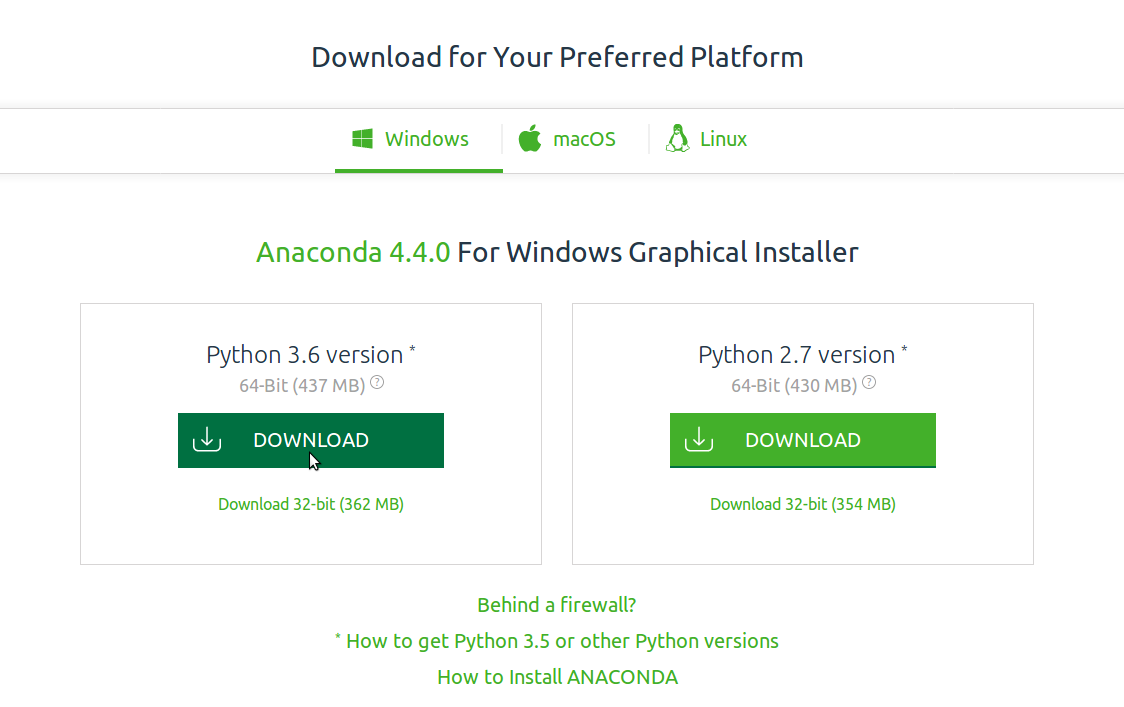
\includegraphics[width=0.6\textwidth]{anaconda_download}
\end{center}
}



\frame{
\frametitle{Primero lo primero}
Depende de la forma en la que hayan instalado python, pueden comenzar a usarlo de diferentes maneras, como por la línea de comandos (cmd). Si instalaron anaconda, podrán entrar desde allí.
\begin{center}
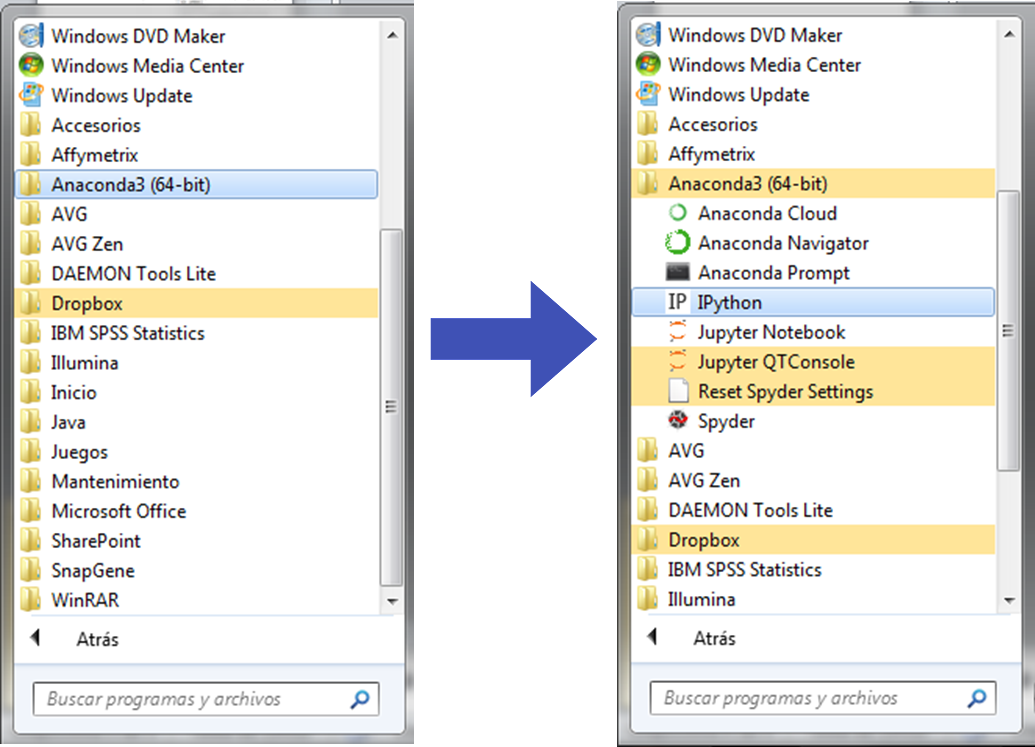
\includegraphics[width=0.8\textwidth]{menu_ipython}
\end{center}
}



\frame{
\frametitle{Python en consola}
\begin{itemize}
	\item Esta pantalla es la consola de python.
\end{itemize}
\begin{center}
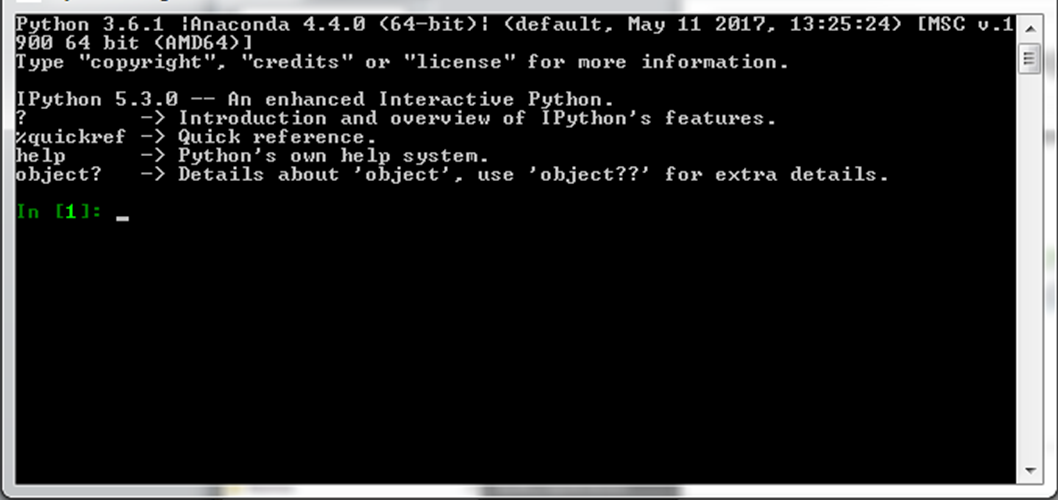
\includegraphics[width=\textwidth]{ipython}
\end{center}
\vspace{-0.5cm}
\begin{itemize}
	\item Aquí podrán escribir los comandos directamente para que python los interprete y ejecute.
\end{itemize}
}


\subsubsection{El "{}Hola Mundo"{}}


\frame{
\frametitle{Hola Mundo}
\framesubtitle{en Pythoh}

\begin{itemize}
	\item El primer programa por excelencia, el "{}Hola Mundo"{}
	\item La consola recibe la instrucción de mostrar en la pantalla un mensaje.
\end{itemize}

\colorbox{source}{\parbox{\textwidth}{
\ttfamily
\mbox{}\\
\textbf{\textcolor{Blue}{print}}\textcolor{BrickRed}{(}\texttt{\textcolor{Red}{"{}Hola\ Mundo"{}}}\textcolor{BrickRed}{)} \\
\mbox{}
}}
\begin{itemize}
	\item El mensaje debe ir entre comillas.
\end{itemize}
}



\frame{
\frametitle{El editor}
\small
Python, al igual que la mayoría de los lenguajes de programación, no necesita nada más complejo que un bloc de notas. Pero existen un sinnúmero de opciones, pueden usar la que más les guste.

Si instalaron anaconda, y no tienen un editor preferido, pueden probar \emph{Spyder}.
\begin{center}
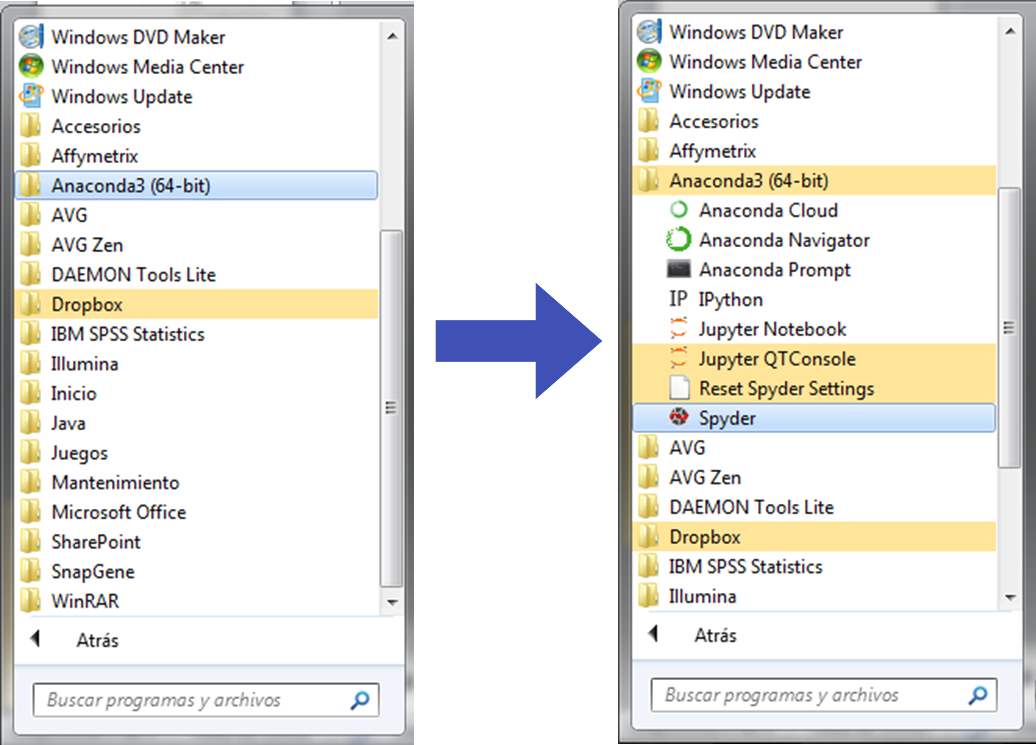
\includegraphics[width=0.75\textwidth]{menu_spyder}
\end{center}
}



\frame{
\frametitle{Spyder}
\begin{itemize}
	\item Spyder cuenta con una consola en la que se pueden ejecutar comandos, o lo que se esté escribiendo en el editor.
	\item Además, cuenta con un apartado de ayuda para las funciones de Python.
\end{itemize}
\begin{center}
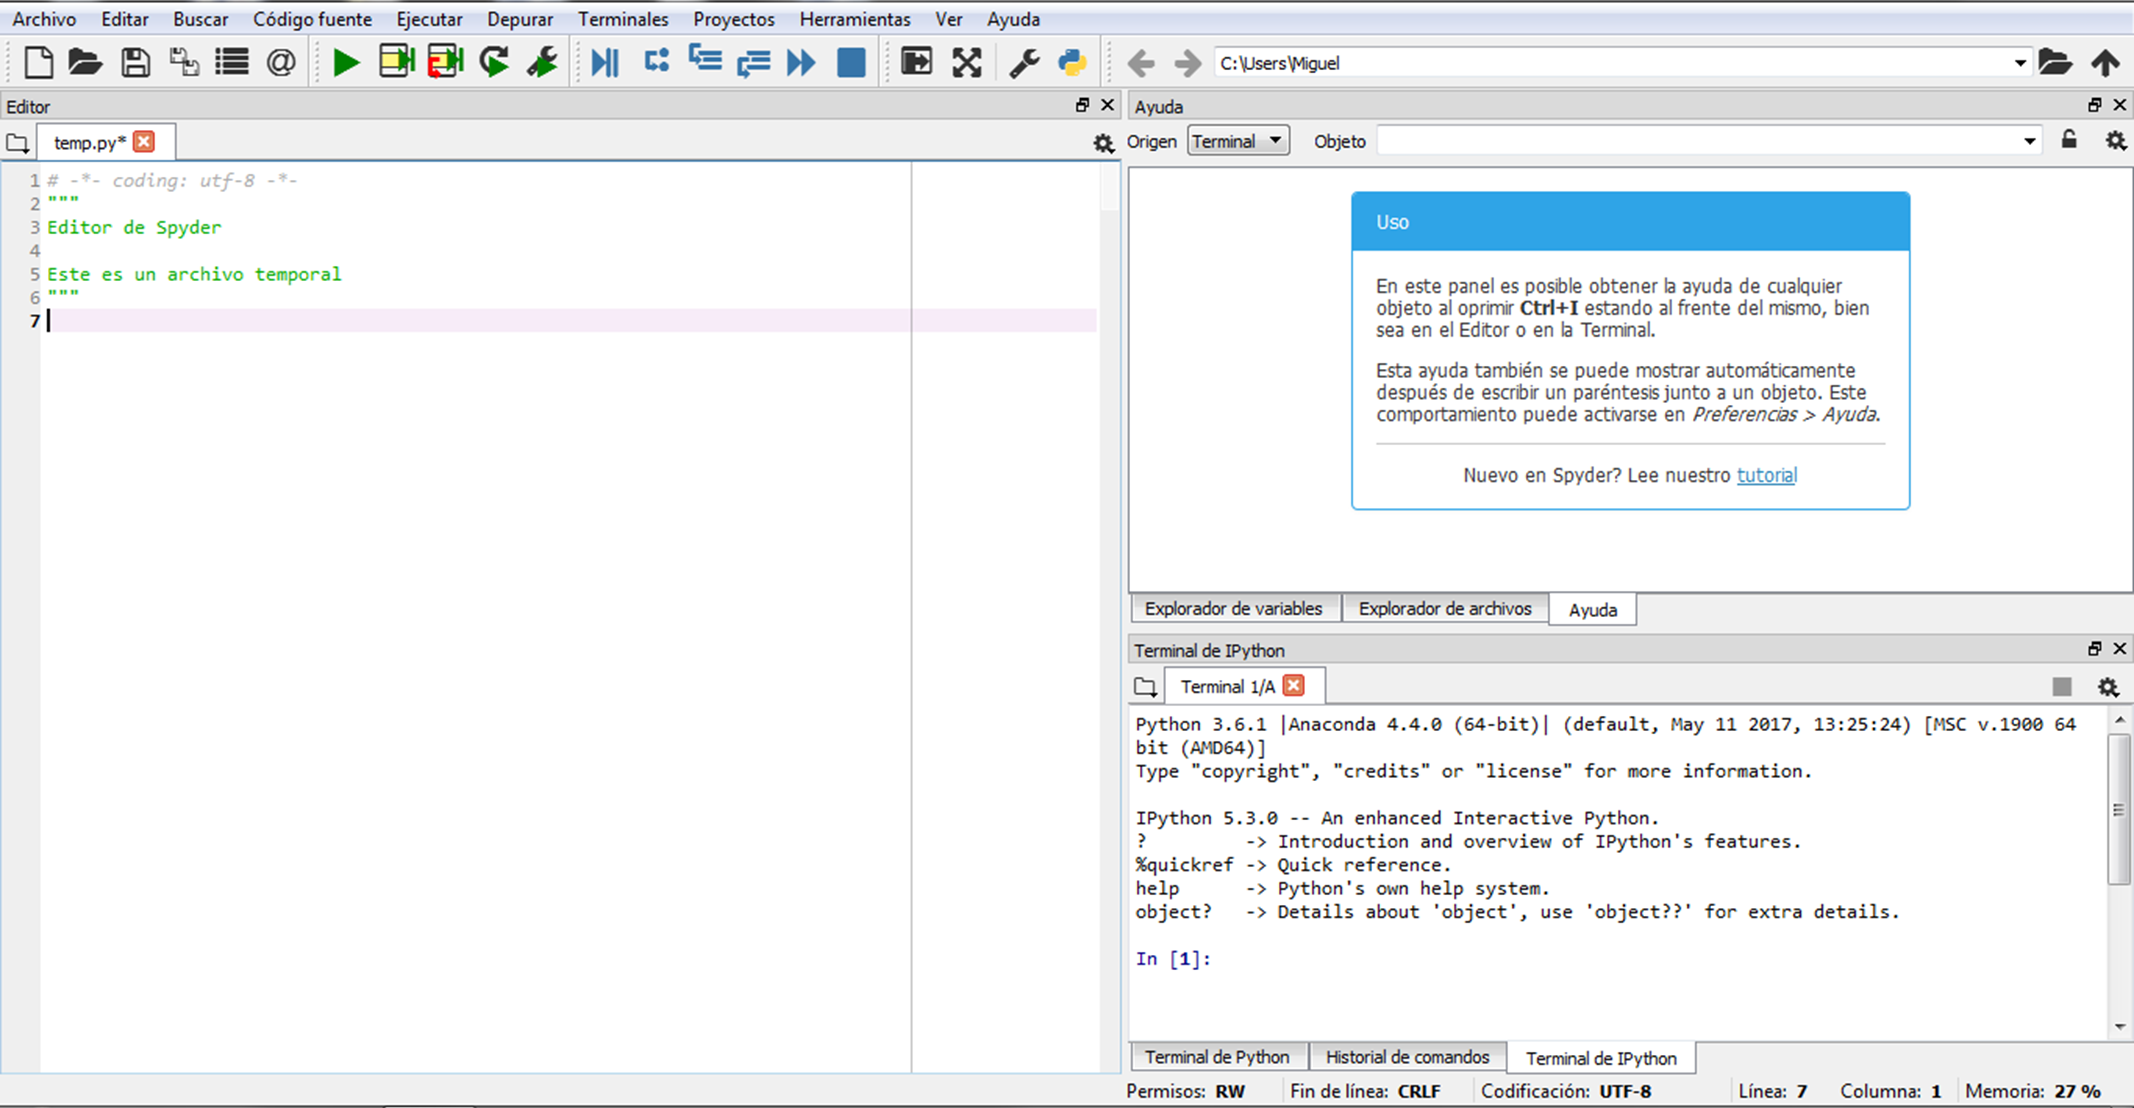
\includegraphics[width=\textwidth]{spyder}
\end{center}
}



\frame{
\frametitle{El editor}
\begin{itemize}
	\item Dentro del editor podemos escribir una serie de comandos que queremos que se ejecuten.
	\item Serán leídos e interpretados en orden, uno tras otro.
\end{itemize}
\colorbox{source}{\parbox{\textwidth}{
\ttfamily
\mbox{}\\
\textbf{\textcolor{Blue}{print}}\textcolor{BrickRed}{(}\texttt{\textcolor{Red}{"{}De\ ola\ en\ ola,"{}}}\textcolor{BrickRed}{)} \\
\mbox{}\textbf{\textcolor{Blue}{print}}\textcolor{BrickRed}{(}\texttt{\textcolor{Red}{"{}de\ rama\ en\ rama,"{}}}\textcolor{BrickRed}{)} \\
\mbox{}\textbf{\textcolor{Blue}{print}}\textcolor{BrickRed}{(}\texttt{\textcolor{Red}{"{}el\ viento\ silba"{}}}\textcolor{BrickRed}{)} \\
\mbox{}\textbf{\textcolor{Blue}{print}}\textcolor{BrickRed}{(}\texttt{\textcolor{Red}{"{}cada\ mañana."{}}}\textcolor{BrickRed}{)} \\
\mbox{}
}}
}



\frame{
\frametitle{Spyder}
\begin{itemize}
	\item Una vez que se escriben las instrucciones, se puede ejecutar el archivo completo.
	\item Varios editores cuentan con esta función.
\end{itemize}
\begin{center}
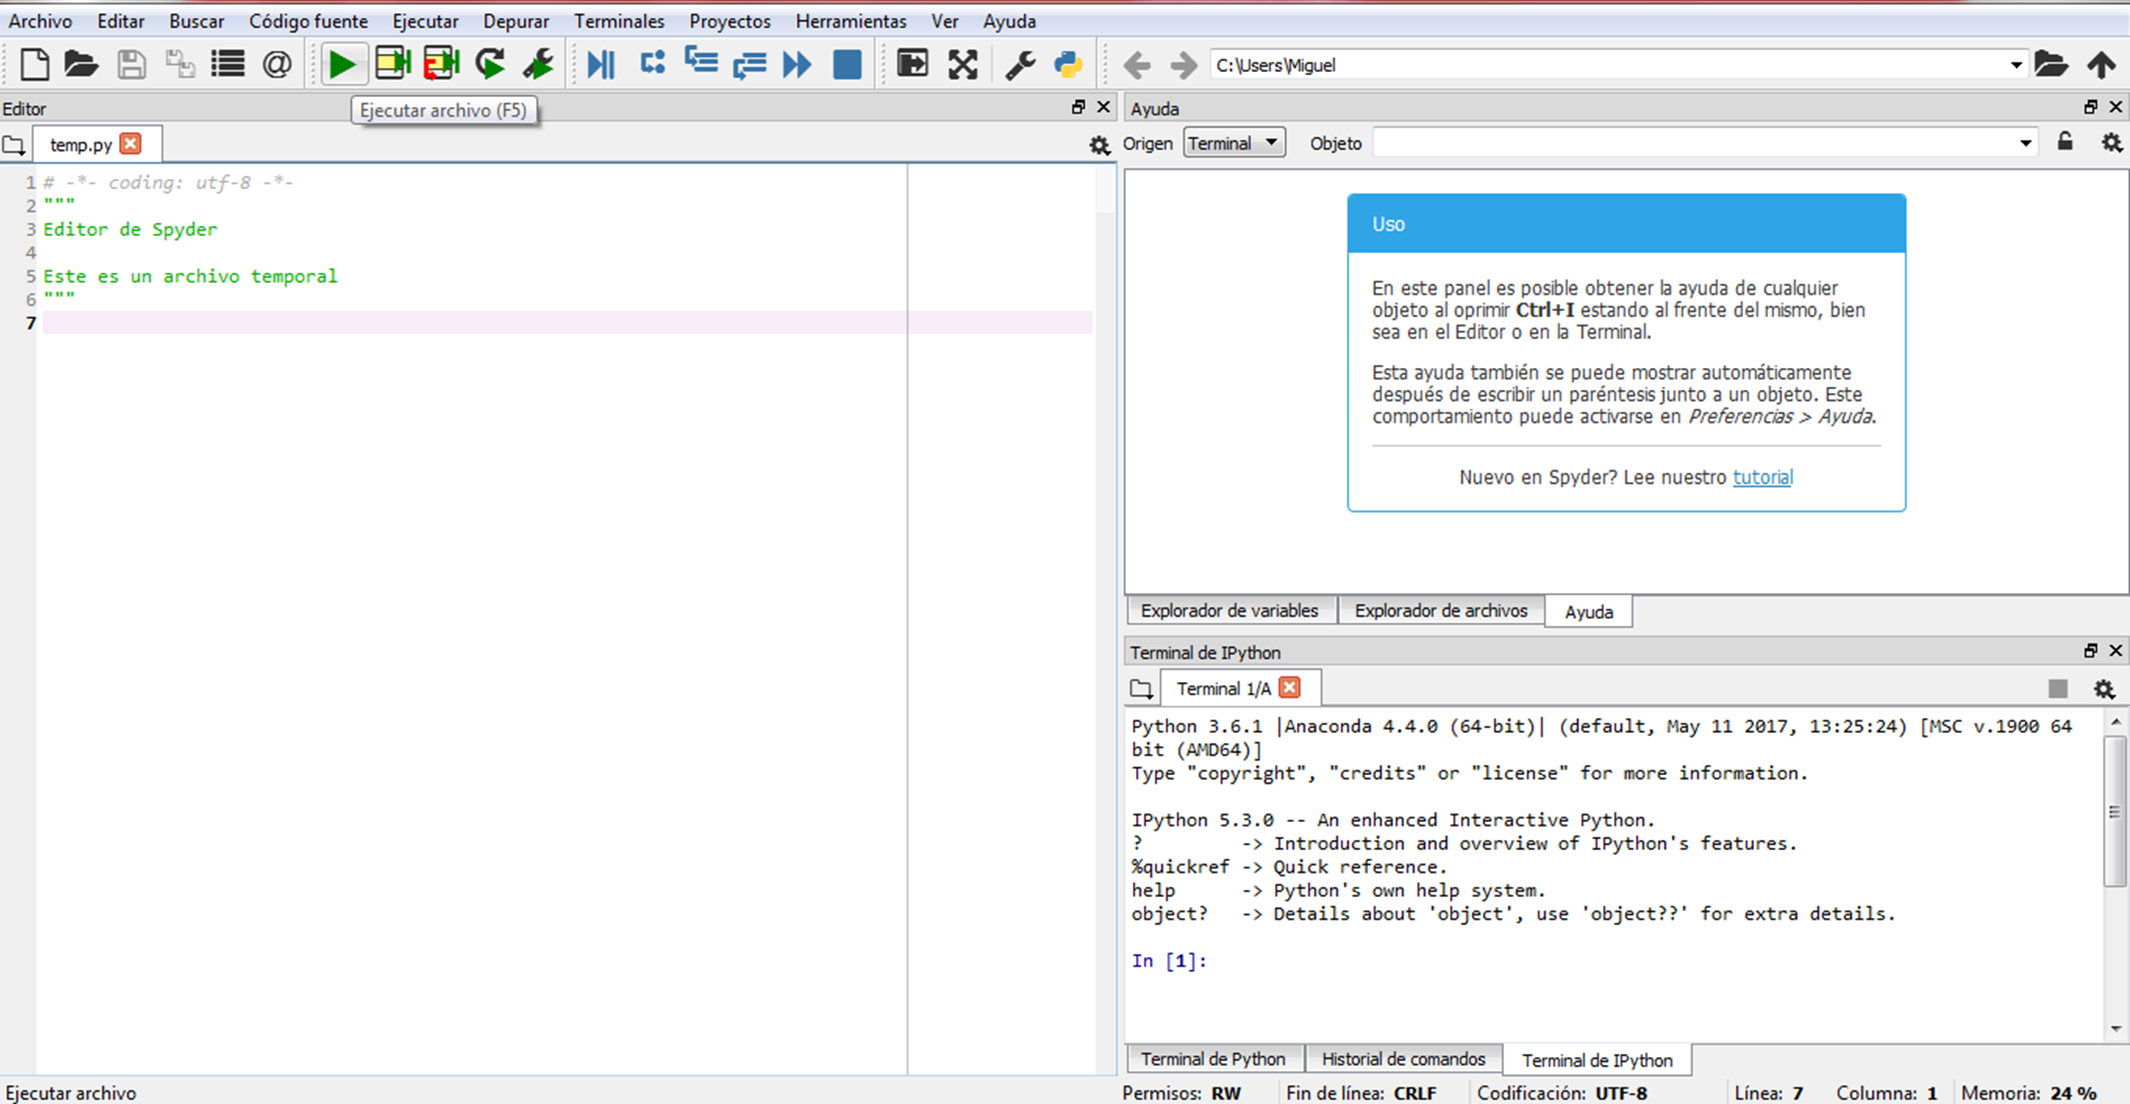
\includegraphics[width=\textwidth]{spyder_run}
\end{center}
}




\subsection{Operaciones}


\frame{
\frametitle{Operaciones}
\begin{itemize}
	\item Python también es capaz de hacer operaciones matemáticas, cual si fuera una calculadora simple.
\end{itemize}
\colorbox{source}{\parbox{\textwidth}{
\ttfamily
\mbox{}\\
\textbf{\textcolor{Blue}{print}}\textcolor{BrickRed}{(}\textcolor{Purple}{2}\ \textcolor{BrickRed}{+}\ \textcolor{Purple}{2}\textcolor{BrickRed}{)} \\
\mbox{}\textbf{\textcolor{Blue}{print}}\textcolor{BrickRed}{(}\textcolor{Purple}{3}\ \textcolor{BrickRed}{*}\ \textcolor{Purple}{4}\textcolor{BrickRed}{)} \\
\mbox{}\textbf{\textcolor{Blue}{print}}\textcolor{BrickRed}{(}\textcolor{Purple}{100}\ \textcolor{BrickRed}{-}\ \textcolor{Purple}{1}\textcolor{BrickRed}{)} \\
\mbox{}
}}
\begin{itemize}
	\item Es importante notar que en este caso, no se usan comillas en el interior de la función {\tt \textbf{print()}}.
\end{itemize}
}



\frame{
\frametitle{Operaciones}
\begin{itemize}
	\item La razón, es que las comillas se utilizan cuando se está manejando texto, los números, para hacer operaciones, se deben tomar como números.
\end{itemize}
\colorbox{source}{\parbox{\textwidth}{
\ttfamily
\mbox{}\\
\textbf{\textcolor{Blue}{print}}\textcolor{BrickRed}{(}\texttt{\textcolor{Red}{"{}2"{}}}\ \textcolor{BrickRed}{+}\ \texttt{\textcolor{Red}{"{}2"{}}}\textcolor{BrickRed}{)} \\
\mbox{}\textbf{\textcolor{Blue}{print}}\textcolor{BrickRed}{(}\texttt{\textcolor{Red}{"{}3\ *\ 4"{}}}\textcolor{BrickRed}{)} \\
\mbox{}\textbf{\textcolor{Blue}{print}}\textcolor{BrickRed}{(}\texttt{\textcolor{Red}{"{}100"{}}}\ \textcolor{BrickRed}{-}\ \textcolor{Purple}{1}\textcolor{BrickRed}{)} \\
\mbox{}
}}
}
\note{
\begin{itemize}
	\item Para el primer ejemplo de esta diapositiva, notarán que el resultado es {\tt \textbf{22}}, esto es debido a que, cuando se está trabajando texto (entre comillas) la operación {\tt \textbf{+}} es una operación de concatenación. Es decir, junta en texto.
	\item Para el segundo ejemplo, se mostrará en pantalla el texto de la operación, no se evaluará nada, al poner comillas, esos ya no son números ni operaciones, es texto.
	\item El último ejemplo provocará un error, Python no sabe hacer operaciones entre texto y números.
\end{itemize}
}



\frame{
\frametitle{Operaciones}
\begin{itemize}
	\item Ambas formas se pueden combinar dentro de la función {\tt \textbf{print()}}.
\end{itemize}
\colorbox{source}{\parbox{\textwidth}{
\ttfamily
\mbox{}\\
\textbf{\textcolor{Blue}{print}}\textcolor{BrickRed}{(}\texttt{\textcolor{Red}{"{}2\ +\ 2\ ="{}}}\textcolor{BrickRed}{,}\ \textcolor{Purple}{2}\ \textcolor{BrickRed}{+}\ \textcolor{Purple}{2}\textcolor{BrickRed}{)} \\
\mbox{}\textbf{\textcolor{Blue}{print}}\textcolor{BrickRed}{(}\texttt{\textcolor{Red}{"{}3\ *\ 4\ ="{}}}\textcolor{BrickRed}{,}\ \textcolor{Purple}{3}\ \textcolor{BrickRed}{*}\ \textcolor{Purple}{4}\textcolor{BrickRed}{)} \\
\mbox{}\textbf{\textcolor{Blue}{print}}\textcolor{BrickRed}{(}\texttt{\textcolor{Red}{"{}100\ -\ 1\ ="{}}}\textcolor{BrickRed}{,}\ \textcolor{Purple}{100}\ \textcolor{BrickRed}{-}\ \textcolor{Purple}{1}\textcolor{BrickRed}{)} \\
\mbox{}
}}
\begin{itemize}
	\item Es importante notar que el texto y los números están separados por una coma.
\end{itemize}
}
\note{
\begin{itemize}
	\item La función {\tt \textbf{print()}} puede recibir varias cosas para mostrar en la pantalla, todas ellas separadas por coma, de esa manera, se separan las entradas.
	\item En el ejemplo estamos mandando tanto texto, como una operación, cada argumento (separado por coma) que mandamos, se evaluará y luego se mostrará en la pantalla.
	\item Si omitimos la coma, se producirá un error, ya que Python no sabe evaluar texto en combinación con una operación matemática.
\end{itemize}
}



\frame{
\frametitle{}
Entonces se tienen:
\begin{itemize}
	\item Palabras, el texto que se debe manejar entre comillas.
	\item Números y operaciones, que deben ir sin comillas para que se evalúen.
\end{itemize}
~

~¿Qué hay de las palabras sin comillas?

\colorbox{source}{\parbox{\textwidth}{
\ttfamily
\mbox{}\\
\textbf{\textcolor{Blue}{print}}\textcolor{BrickRed}{(}Hola\textcolor{BrickRed}{)} \\
\mbox{}
}}
}
\note{
Esto provocará un error.
}


\subsection{Variables}


\frame{
\frametitle{Variables}
\begin{itemize}
	\item Las variables son palabras (o cualquier combinación de letras en realidad) que se utilizan para guardar valores.
	\item Cualquier valor o el resultado de cualquier operación puede ser asignado a una variable.
	\item Los valores se asignan con el símbolo {\tt \textbf{=}}
\end{itemize}
\colorbox{source}{\parbox{\textwidth}{
\ttfamily
\mbox{}\\
nombre\ \textcolor{BrickRed}{=}\ \texttt{\textcolor{Red}{"{}Juan\ Hernández\ Hernández"{}}} \\
\mbox{}suma\ \textcolor{BrickRed}{=}\ \textcolor{Purple}{2}\ \textcolor{BrickRed}{+}\ \textcolor{Purple}{3} \\
\mbox{}\textbf{\textcolor{Blue}{print}}\textcolor{BrickRed}{(}\texttt{\textcolor{Red}{"{}Hola"{}}}\ \textcolor{BrickRed}{,}\ nombre\textcolor{BrickRed}{)} \\
\mbox{}\textbf{\textcolor{Blue}{print}}\textcolor{BrickRed}{(}\texttt{\textcolor{Red}{"{}2\ +\ 3\ ="{}}}\textcolor{BrickRed}{,}\ suma\textcolor{BrickRed}{)} \\
\mbox{}
}}
}
\note{
\begin{itemize}
	\item Las variables se "{}evalúan"{} como si fueran operaciones.
	\item En los ejemplos vemos que se utilizan las variables dentro de la función {\tt \textbf{print()}} de la misma manera que las operaciones. Y de la misma manera, se procesan (y se reemplaza por su valor) antes de ser mostradas en pantalla.
\end{itemize}
}



\frame{
\frametitle{Variables}
\begin{itemize}
	\item Las variables también pueden ser utilizadas para asignar otras variables.
	\item O incluso para cambiar su propio valor
\end{itemize}
\colorbox{source}{\parbox{\textwidth}{
\ttfamily
\mbox{}\\
x\ \textcolor{BrickRed}{=}\ \textcolor{Purple}{2}\ \textcolor{BrickRed}{+}\ \textcolor{Purple}{3} \\
\mbox{}y\ \textcolor{BrickRed}{=}\ x\ \textcolor{BrickRed}{+}\ \textcolor{Purple}{5} \\
\mbox{}\textbf{\textcolor{Blue}{print}}\textcolor{BrickRed}{(}\texttt{\textcolor{Red}{"{}x\ ="{}}}\textcolor{BrickRed}{,}\ x\textcolor{BrickRed}{)} \\
\mbox{}\textbf{\textcolor{Blue}{print}}\textcolor{BrickRed}{(}\texttt{\textcolor{Red}{"{}y\ ="{}}}\textcolor{BrickRed}{,}\ y\textcolor{BrickRed}{)} \\
\mbox{} \\
\mbox{}y\ \textcolor{BrickRed}{=}\ y\ \textcolor{BrickRed}{+}\ \textcolor{Purple}{10} \\
\mbox{}\textbf{\textcolor{Blue}{print}}\textcolor{BrickRed}{(}\texttt{\textcolor{Red}{"{}y\ ="{}}}\textcolor{BrickRed}{,}\ y\textcolor{BrickRed}{)} \\
\mbox{}
}}
}



%~ \frame{
%~ \frametitle{Variables}
%~ \begin{alertblock}{IMPORTANTE}
	%~ Todos los comandos que utilicen en Python sin asignarlos a una variable, se ejecutarán pero no tendrán forma de hacer referencia a ellos, se perderán. Por norma general, asignen lo que hagan dentro de variables.
%~ \end{alertblock}
%~ \colorbox{source}{\parbox{\textwidth}{
%~ \ttfamily
%~ \mbox{}\\
%~ x\ \textcolor{BrickRed}{=}\ \textcolor{Purple}{2}\ \textcolor{BrickRed}{+}\ \textcolor{Purple}{3} \\
%~ \mbox{}y\ \textcolor{BrickRed}{=}\ x\ \textcolor{BrickRed}{+}\ \textcolor{Purple}{5} \\
%~ \mbox{}\textbf{\textcolor{Blue}{print}}\textcolor{BrickRed}{(}\texttt{\textcolor{Red}{"{}2\ +\ 3\ ="{}}}\textcolor{BrickRed}{,}\ x\textcolor{BrickRed}{)} \\
%~ \mbox{}\textbf{\textcolor{Blue}{print}}\textcolor{BrickRed}{(}\texttt{\textcolor{Red}{"{}x\ +\ 5\ ="{}}}\textcolor{BrickRed}{,}\ y\textcolor{BrickRed}{)} \\
%~ \mbox{} \\
%~ \mbox{}z\ \textcolor{BrickRed}{=}\ \textbf{\textcolor{Black}{abs}}\textcolor{BrickRed}{(-}\textcolor{Purple}{10}\textcolor{BrickRed}{)} \\
%~ \mbox{}\textbf{\textcolor{Blue}{print}}\textcolor{BrickRed}{(}\texttt{\textcolor{Red}{"{}valor\ absoluto\ de\ -10\ ="{}}}\textcolor{BrickRed}{,}\ z\textcolor{BrickRed}{)} \\
%~ \mbox{}
%~ }}
%~ }
%~ \note{
%~ \begin{itemize}
	%~ \item En el código de ejemplo, podemos ver cómo todas las sumas son asignadas a una variable.
	%~ \item De igual manera, la función {\tt \textbf{abs()}} se asigna a una variable.
	%~ \item Sin embargo, las funciones {\tt \textbf{print()}} no se asignan.
%~ \end{itemize}
%~ Por regla general, es mejor asignar todo, en particular {\tt \textbf{print()}} es una función que se puede considerar como algo volátil, se muestra en pantalla para nosotros y no se vuelve a usar. Pero ese no es el caso para la mayoría de las funciones.
%~ }


\subsection{Comentarios}


\frame{
\frametitle{Comentarios}
\begin{alertblock}{IMPORTANTE}
	Dejen que su código les hable.
	
	Y háganlo aunque les de flojera.
\end{alertblock}
\colorbox{source}{\parbox{\textwidth}{
\ttfamily
\small
\mbox{}\\
x\ \textcolor{BrickRed}{=}\ \textcolor{Purple}{2}\ \textcolor{BrickRed}{+}\ \textcolor{Purple}{3}\ \textit{\textcolor{Brown}{\#\ A\ x\ se\ le\ asigna\ el\ resultado\ de\ una\ suma.}} \\
\mbox{}y\ \textcolor{BrickRed}{=}\ x\ \textcolor{BrickRed}{+}\ \textcolor{Purple}{5}\ \textit{\textcolor{Brown}{\#\ Se\ puede\ user\ una\ variable\ asignada\ para\ hacer\ \\ \mbox{} \hspace{2cm}\# operaciones.}} \\
\mbox{}\textbf{\textcolor{Blue}{print}}\textcolor{BrickRed}{(}\texttt{\textcolor{Red}{"{}x\ ="{}}}\textcolor{BrickRed}{,}\ x\textcolor{BrickRed}{)}\ \textit{\textcolor{Brown}{\#\ El\ comando\ print()\ sirve\ para\ \\ \mbox{} \hspace{3cm}\# mostrar\ cosas\ en\ pantalla.}} \\
\mbox{}\textbf{\textcolor{Blue}{print}}\textcolor{BrickRed}{(}\texttt{\textcolor{Red}{"{}x\ +\ 5\ ="{}}}\textcolor{BrickRed}{,}\ y\textcolor{BrickRed}{)}\ \textit{\textcolor{Brown}{\#\ Puede\ recibir\ texto\ o\ números,\ \\ \mbox{} \hspace{3cm}\# incluso\ operaciones,\ pero\ separados\ por\ \\ \mbox{} \hspace{3cm}\# comas.}} \\
\mbox{}
}}
}
\note{
\begin{itemize}
\footnotesize
	\item No me canso de repetir lo importante que es esto.
	\item Comentar el código es una de los mejores hábitos que se pueden hacer al comenzar a programar.
	\item Les facilita a recordar lo que hacen las funciones.
	\item Pero más importante que eso, les ayuda a leer su código, incluso si tiene mucho tiempo que lo hicieron. Entre más saben programar y más complejos son sus programas, pueden plasmar en código ideas mas completas, en el momento las tienen bien presentes, pero cuando se regresa, uno se da cuenta que no recuerda exactamente lo que estaba pensando en ese momento ni para qué hizo las cosas que hizo.
	\item También para trabajar en equipo sobre un proyecto mas completo, esto es crucial.
	\item Leer código no comentado es una cosa muy tediosa y difícil. Más aún si es de otra persona.
\end{itemize}
}



\section{Archivos}

\subsection{Corpus}

\frame{
\frametitle{Corpus}
\begin{itemize}
	\item Un corpus es un conjunto de documentos (texto, video, audio, etc.) destinado a la investigación.
	\item La recolección de un corpus depende de lo que se busca estudiar.
	\item Para este curso, contamos con un conjunto de documentos legales, sin embargo, si cuentan con un corpus propio pueden utilizarlo. 
\end{itemize}
}


\frame{
\frametitle{Ruta de archivos}
\begin{itemize}
	\item Es común necesitar la ruta de los archivos.
	\item En Windows, se puede usar SHIFT+CLICK\_DERECHO en un archivo, lo que despliega un menú de opciones en el que aparece: "{}{\tt \textbf{Copiar como ruta de acceso}}"{}
\end{itemize}
\begin{center}
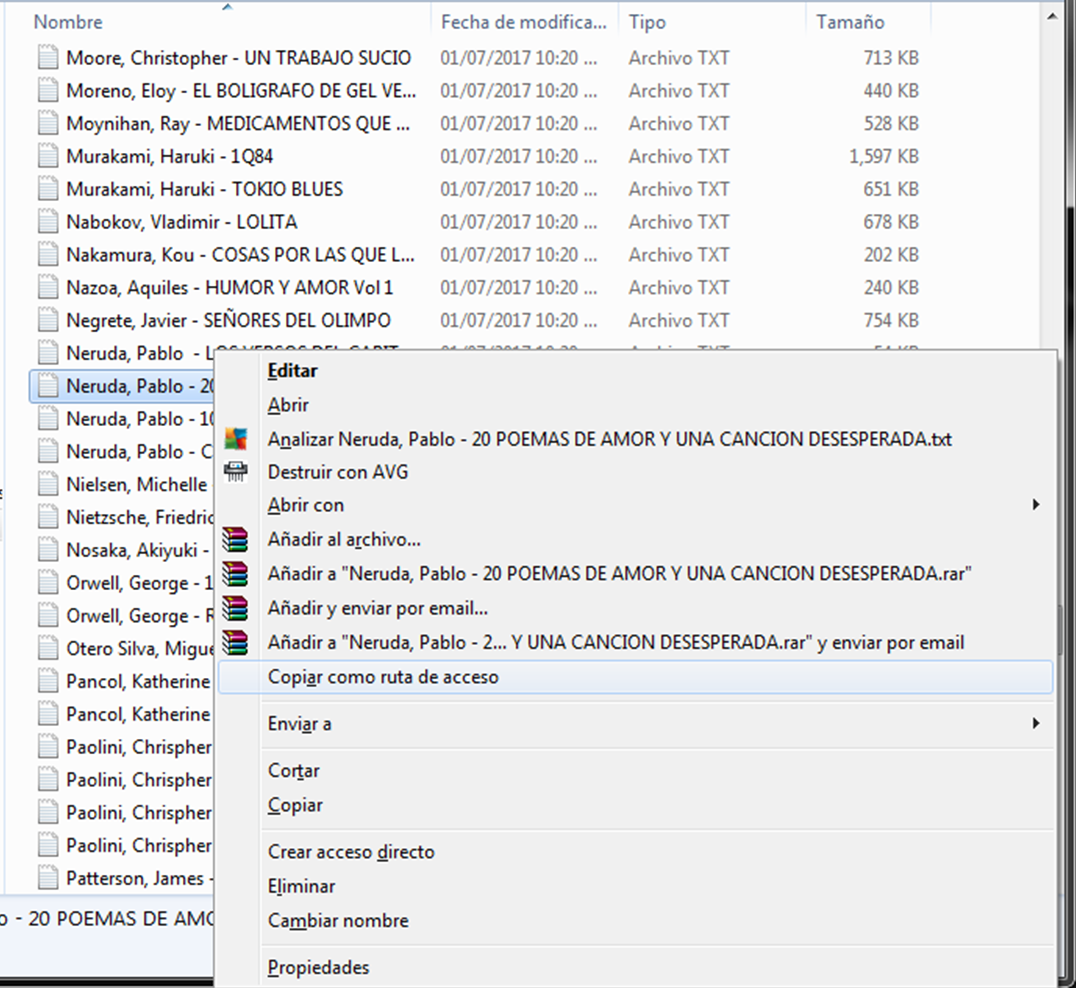
\includegraphics[width=0.6\textwidth]{ruta_completa}
\end{center}
}

\subsection{Lectura de archivos}

\frame{
\frametitle{Lectura de archivos}
\begin{itemize}
	\item Para comenzar a trabajar con un archivo, lo primero que se tiene que hacer es abrirlo.
\end{itemize}
\begin{description}
	\item[IMPORTANTE] Las rutas de los archivos en Windows separan las carpetas con diagonal invertida (`\textbackslash'). Éste es un símbolo especial que no se puede usar así nada mas, más adelante veremos por qué. Por ahora solo recuerden que deben duplicar la diagonal invertida (`\textbackslash\textbackslash' en lugar de `\textbackslash').
\end{description}
\colorbox{source}{\parbox{\textwidth}{
\ttfamily
\small
\mbox{}\\
archivo$\_$abierto\textcolor{BrickRed}{=}\textbf{\textcolor{Black}{open}}\textcolor{BrickRed}{(}\texttt{\textcolor{Red}{"{}C:\textbackslash\textbackslash{}RUTA\textbackslash\textbackslash{}P$\_$IFT$\_$290216$\_$73$\_$Acc.txt"{}}}\textcolor{BrickRed}{)} \\
\mbox{}
}}
}



\frame{
\frametitle{Lectura de archivos}
\begin{itemize}
	\item Ya que el archivo está abierto podemos leer el contenido.
\end{itemize}
\colorbox{source}{\parbox{\textwidth}{
\ttfamily
\small
\mbox{}\\
\mbox{}texto\textcolor{BrickRed}{=}archivo$\_$abierto\textcolor{BrickRed}{.}\textbf{\textcolor{Black}{read}}\textcolor{BrickRed}{()} \\
\mbox{}
}}
\begin{itemize}
	\item {\tt \textbf{read()} es una función de los archivos (debe ser un archivo que haya sido abierto con la función {\tt \textbf{open()}}}) que lee el texto y lo "{}regresa"{}. Esto quiere decir que el resultado puede (o mejor dicho \textbf{debe}) asignarse a una variable, en este caso, la variable {\tt \textbf{texto}}
	\item Es una función que no recibe ningún argumento, por eso los paréntesis vacíos.
\end{itemize}
}



\frame{
\frametitle{Lectura de archivos}
\begin{itemize}
	\item Podemos hacer que Python nos muestre el contenido del archivo, que ahora está en la variable {\tt \textbf{texto}}.
\end{itemize}
\colorbox{source}{\parbox{\textwidth}{
\ttfamily
\mbox{}\\
\textbf{\textcolor{Blue}{print}}\textcolor{BrickRed}{(}texto\textcolor{BrickRed}{)} \\
\mbox{}
}}
\begin{itemize}
	\item Recuerden que en esta ocasión NO se usan comillas, queremos usar la variable {\tt \textbf{texto}} no el texto: \emph{"{}texto"{}}
	\item Finalmente, es importante cerrar el archivo que abrimos en primer lugar:
\end{itemize}
\colorbox{source}{\parbox{\textwidth}{
\ttfamily
\mbox{}\\
archivo$\_$abierto\textcolor{BrickRed}{.}\textbf{\textcolor{Black}{close}}\textcolor{BrickRed}{()} \\
\mbox{}
}}
}



\frame{
\frametitle{Lectura de archivos}
\begin{itemize}
	\item El programa completo se vería algo así:
\end{itemize}
\colorbox{source}{\parbox{\textwidth}{
\ttfamily
\small
\mbox{}\\
archivo$\_$abierto\textcolor{BrickRed}{=}\textbf{\textcolor{Black}{open}}\textcolor{BrickRed}{(}\texttt{\textcolor{Red}{"{}C:\textbackslash\textbackslash{}RUTA\textbackslash\textbackslash{}P$\_$IFT$\_$290216$\_$73$\_$Acc.txt"{} }}\textcolor{BrickRed}{)} \\
\mbox{}texto\textcolor{BrickRed}{=}archivo$\_$abierto\textcolor{BrickRed}{.}\textbf{\textcolor{Black}{read}}\textcolor{BrickRed}{()} \\
\mbox{}\textbf{\textcolor{Blue}{print}}\textcolor{BrickRed}{(}texto\textcolor{BrickRed}{)} \\
\mbox{}archivo$\_$abierto\textcolor{BrickRed}{.}\textbf{\textcolor{Black}{close}}\textcolor{BrickRed}{()} \\
\mbox{}
}}
\begin{itemize}
	\item Más sus respectivos comentarios
\end{itemize}
}


\subsection{Escritura de archivos}


\frame{
\frametitle{Escritura de archivos}
\begin{itemize}
	\item El proceso de escritura es similar, pero se distingue desde la forma en la que se abre el archivo
\end{itemize}
\colorbox{source}{\parbox{\textwidth}{
\ttfamily
\small
\mbox{}\\
archivo$\_$abierto\textcolor{BrickRed}{=}\textbf{\textcolor{Black}{open}}\textcolor{BrickRed}{(}\texttt{\textcolor{Red}{"{}C:\textbackslash\textbackslash{}RUTA\textbackslash\textbackslash{}mi$\_$archivo$\_$nuevo.txt"{}}}\textcolor{BrickRed}{,}\texttt{\textcolor{Red}{"{}w"{}}}\textcolor{BrickRed}{)} \\
\mbox{}
}}
\begin{itemize}
	\item Noten dos cosas.
	\item Primero, la \emph{`w'} como segundo argumento de la función {\tt \textbf{open()}}. Esa \emph{`w'} significa \emph{write}, y se usa para abrir el archivo en modo escritura (si se omite, como en el caso anterior, por defecto los archivos se abren en modo lectura: {\tt \textbf{r}}).
	\item Segundo, el nombre del archivo. NO hagan esto con un archivo existente. Cuando se abre un archivo en modo escritura, se crea como nuevo, y Python no pregunta si quieres sobreescribir, lo hace.
\end{itemize}
}



\frame{
\frametitle{Escritura de archivos}
\begin{itemize}
	\item Para escribir en el archivo, usaremos la función {\tt \textbf{write()}}.
\end{itemize}
\colorbox{source}{\parbox{\textwidth}{
\ttfamily
\small
\mbox{}\\
archivo$\_$abierto\textcolor{BrickRed}{=}\textbf{\textcolor{Black}{open}}\textcolor{BrickRed}{(}\texttt{\textcolor{Red}{"{}C:\textbackslash\textbackslash{}RUTA\textbackslash\textbackslash{}mi$\_$archivo$\_$nuevo.txt"{}}}\textcolor{BrickRed}{,}\texttt{\textcolor{Red}{"{}w"{}}}\textcolor{BrickRed}{)} \\
\mbox{}archivo$\_$abierto\textcolor{BrickRed}{.}\textbf{\textcolor{Black}{write}}\textcolor{BrickRed}{(}\texttt{\textcolor{Red}{"{}Esto\ se\ escribe\ en\ el\ archivo"{}}}\textcolor{BrickRed}{)} \\
\mbox{}archivo$\_$abierto\textcolor{BrickRed}{.}\textbf{\textcolor{Black}{write}}\textcolor{BrickRed}{(}\texttt{\textcolor{Red}{"{}Esto\ tambien"{}}}\textcolor{BrickRed}{)} \\
\mbox{}
}}
\begin{itemize}
	\item La función {\tt \textbf{write()}} es muy parecida a {\tt \textbf{print()}}, con la diferencia de que manda el texto al archivo en lugar de a la pantalla.
	\item Para ver los cambios en su archivo, no olviden cerrarlo.
\end{itemize}
\colorbox{source}{\parbox{\textwidth}{
\ttfamily
\mbox{}\\
archivo$\_$abierto\textcolor{BrickRed}{.}\textbf{\textcolor{Black}{close}}\textcolor{BrickRed}{()} \\
\mbox{}
}}
}



\frame{
\frametitle{Escritura de archivos}
\begin{itemize}
	\item Si abren su archivo verán lo que escribieron, y lo más probable es que se topen con algo como esto.
\end{itemize}
\colorbox{output}{\parbox{\textwidth}{
\ttfamily
\mbox{}\\
Esto se escribe en el archivoEsto tambien \\
\mbox{}
}}
\begin{itemize}
	\item Probablemente este no era el resultado que esperaban.
	\item Una diferencia entre {\tt \textbf{print()}} y {\tt \textbf{write()}} es que {\tt \textbf{write()}} no añade un salto de línea en el archivo como {\tt \textbf{print()}} en la pantalla.
\end{itemize}
}



\frame{
\frametitle{Escritura de archivos}
\small
\begin{itemize}
	\item Para agregar saltos de línea a voluntad se usa el símbolo: {\tt \textbf{\textbackslash n}}
	\item Por lo tanto, el programa anterior, sería mejor escribirlo algo así:
\end{itemize}
\colorbox{source}{\parbox{\textwidth}{
\ttfamily
\footnotesize
\mbox{}\\
archivo$\_$abierto\textcolor{BrickRed}{=}\textbf{\textcolor{Black}{open}}\textcolor{BrickRed}{(}\texttt{\textcolor{Red}{"{}C:\textbackslash\textbackslash{}RUTA\textbackslash\textbackslash{}mi$\_$archivo$\_$nuevo.txt"{}}}\textcolor{BrickRed}{,}\texttt{\textcolor{Red}{"{}w"{}}}\textcolor{BrickRed}{)} \\ \\
\mbox{}archivo$\_$abierto\textcolor{BrickRed}{.}\textbf{\textcolor{Black}{write}}\textcolor{BrickRed}{(}\texttt{\textcolor{Red}{"{}Esto\ se\ escribe\ en\ el\ archivo\textbackslash{}n"{}}}\textcolor{BrickRed}{)} \\
\mbox{}archivo$\_$abierto\textcolor{BrickRed}{.}\textbf{\textcolor{Black}{write}}\textcolor{BrickRed}{(}\texttt{\textcolor{Red}{"{}Esto\ tambien\textbackslash{}n"{}}}\textcolor{BrickRed}{)} \\
\mbox{}archivo$\_$abierto\textcolor{BrickRed}{.}\textbf{\textcolor{Black}{write}}\textcolor{BrickRed}{(}\texttt{\textcolor{Red}{"{}Mira,\ puedo\ escribir\ \textbackslash{}"{}comillas\textbackslash{}"{}\textbackslash{}n"{}}}\textcolor{BrickRed}{)} \\
\mbox{}archivo$\_$abierto\textcolor{BrickRed}{.}\textbf{\textcolor{Black}{write}}\textcolor{BrickRed}{(}\texttt{\textcolor{Red}{"{}Gracias\ a\ la\ diagonal\ invertida:\ \textbackslash\textbackslash\ \textbackslash{}n"{}}}\textcolor{BrickRed}{)} \\ \\
\mbox{}archivo$\_$abierto\textcolor{BrickRed}{.}\textbf{\textcolor{Black}{close}}\textcolor{BrickRed}{()} \\
\mbox{}
}}
\begin{itemize}
	\item Al agregar un {\tt \textbf{\textbackslash n}} al final de cada texto en el que se use la función {\tt \textbf{write()}}, se obtiene el mismo comportamiento que con {\tt \textbf{print()}}
	\item Como ven, la diagonal invertida es un símbolo especial. También se puede usar para escribir comillas dentro de los mensajes y que no se malinterpreten como el cierre de comillas.
\end{itemize}
}
\note{
\begin{itemize}
	\item La diagonal invertida es un símbolo especial, recuerden.
	\item Este es un ejemplo del por qué, dependiendo de la tecla que siga a la diagonal invertida (en este caso la `n') tendrá diferente significado.
	\item {\tt \textbf{\textbackslash n}} quiere decir salto de línea, otro ejemplo es {\tt \textbf{\textbackslash t}}, que quiere decir tabulador, o la misma  {\tt \textbf{\textbackslash \textbackslash}} que quiere decir diagonal invertida.
\end{itemize}
}



\subsection*{}



\frame{
\frametitle{Ejemplo}
\colorbox{source}{\parbox{\textwidth}{
\ttfamily
\mbox{}\\
c\textcolor{BrickRed}{=}\texttt{\textcolor{Red}{"{}C:\textbackslash{}\textbackslash{}Users\textbackslash{}\textbackslash{}user\textbackslash{}\textbackslash{}Desktop\textbackslash{}\textbackslash{}Documentos\textbackslash{}\textbackslash{}"{}}} \\
\mbox{}e\textcolor{BrickRed}{=}\texttt{\textcolor{Red}{"{}P$\_$IFT$\_$290216$\_$73$\_$Acc.txt"{}}} \\
\mbox{}s\textcolor{BrickRed}{=}\texttt{\textcolor{Red}{"{}archivo$\_$nuevo.txt"{}}} \\
\mbox{}e2\textcolor{BrickRed}{=}\textbf{\textcolor{Black}{open}}\textcolor{BrickRed}{(}c\textcolor{BrickRed}{+}e\textcolor{BrickRed}{,}\texttt{\textcolor{Red}{"{}r"{}}}\textcolor{BrickRed}{)} \\
\mbox{}s2\textcolor{BrickRed}{=}\textbf{\textcolor{Black}{open}}\textcolor{BrickRed}{(}c\textcolor{BrickRed}{+}s\textcolor{BrickRed}{,}\texttt{\textcolor{Red}{"{}w"{}}}\textcolor{BrickRed}{)} \\
\mbox{}t\textcolor{BrickRed}{=}e2\textcolor{BrickRed}{.}\textbf{\textcolor{Black}{read}}\textcolor{BrickRed}{()} \\
\mbox{}t2\textcolor{BrickRed}{=}t \\
\mbox{}s2\textcolor{BrickRed}{.}\textbf{\textcolor{Black}{write}}\textcolor{BrickRed}{(}t2\textcolor{BrickRed}{)} \\
\mbox{}e2\textcolor{BrickRed}{.}\textbf{\textcolor{Black}{close}}\textcolor{BrickRed}{()} \\
\mbox{}s2\textcolor{BrickRed}{.}\textbf{\textcolor{Black}{close}}\textcolor{BrickRed}{()} \\
\mbox{}
}}
}
\note{
\begin{itemize}
	\item Este es un programa de ejemplo que abre dos archivos. Uno para leer y otro para escribir
	\item Toma el texto del primer archivo y lo escribe en el segundo.
	\item Es una copia de archivos vaya.
\end{itemize}
}



\frame{
\frametitle{Ejemplo}
\colorbox{source}{\parbox{\textwidth}{
\ttfamily
\small
\mbox{}\\
carpeta$\_$nombre\textcolor{BrickRed}{=}\texttt{\textcolor{Red}{"{}C:\textbackslash{}\textbackslash{}Users\textbackslash{}\textbackslash{}user\textbackslash{}\textbackslash{}Desktop\textbackslash{}\textbackslash{}Documentos\textbackslash{}\textbackslash{}"{}}} \\
\mbox{}archivo$\_$nombre\textcolor{BrickRed}{=}\texttt{\textcolor{Red}{"{}P$\_$IFT$\_$290216$\_$73$\_$Acc.txt"{}}} \\
\mbox{}salida$\_$nombre\textcolor{BrickRed}{=}\texttt{\textcolor{Red}{"{}archivo$\_$nuevo.txt"{}}} \\
\mbox{} \\
\mbox{}entrada$\_$abierto\textcolor{BrickRed}{=}\textbf{\textcolor{Black}{open}}\textcolor{BrickRed}{(}carpeta$\_$nombre\textcolor{BrickRed}{+}archivo$\_$nombre\textcolor{BrickRed}{,}\texttt{\textcolor{Red}{"{}r"{}}}\textcolor{BrickRed}{)} \\
\mbox{}salida$\_$abierto\textcolor{BrickRed}{=}\textbf{\textcolor{Black}{open}}\textcolor{BrickRed}{(}carpeta$\_$nombre\textcolor{BrickRed}{+}salida$\_$nombre\textcolor{BrickRed}{,}\texttt{\textcolor{Red}{"{}w"{}}}\textcolor{BrickRed}{)} \\
\mbox{} \\
\mbox{}texto$\_$entrada\textcolor{BrickRed}{=}entrada$\_$abierto\textcolor{BrickRed}{.}\textbf{\textcolor{Black}{read}}\textcolor{BrickRed}{()} \\
\mbox{}texto$\_$salida\textcolor{BrickRed}{=}texto$\_$entrada \\
\mbox{} \\
\mbox{}salida$\_$abierto\textcolor{BrickRed}{.}\textbf{\textcolor{Black}{write}}\textcolor{BrickRed}{(}texto$\_$salida\textcolor{BrickRed}{)} \\
\mbox{} \\
\mbox{}entrada$\_$abierto\textcolor{BrickRed}{.}\textbf{\textcolor{Black}{close}}\textcolor{BrickRed}{()} \\
\mbox{}salida$\_$abierto\textcolor{BrickRed}{.}\textbf{\textcolor{Black}{close}}\textcolor{BrickRed}{()} \\
\mbox{}
}}
}
\note{
\begin{itemize}
	\item Este es el mismo programa que el anterior.
	\item Pero quiero que noten cómo es más fácil leer un programa en el que las variables tienen nombres útiles con respecto a para lo que se usan.
	\item Ambos programas son correctos y hacen lo mismo, pero un programa como este segundo es mucho más recomendable, se vuelve más fácil de leer.
	\item Y eso aún si agregarle comentarios. Pongan comentarios.
\end{itemize}
}



\frame{
\frametitle{Manejo de archivos}
\begin{itemize}
	\item Aquí presentaré un código con otra manera de trabajar con un archivo abierto.
	\item Esta forma tiene la ventaja de ser mas clara.
	\item Y también más fácil ya que maneja por si misma el cierre del archivo.
\end{itemize}
\colorbox{source}{\parbox{\textwidth}{
\ttfamily
\small
\mbox{}\\
carpeta$\_$nombre\textcolor{BrickRed}{=}\texttt{\textcolor{Red}{"{}C:\textbackslash{}\textbackslash{}Users\textbackslash{}\textbackslash{}user\textbackslash{}\textbackslash{}Desktop\textbackslash{}\textbackslash{}Documentos\textbackslash{}\textbackslash{}"{}}} \\
\mbox{}archivo$\_$nombre\textcolor{BrickRed}{=}\texttt{\textcolor{Red}{"{}P$\_$IFT$\_$290216$\_$73$\_$Acc.txt"{}}} \\
\mbox{} \\
\mbox{}with\ \textbf{\textcolor{Black}{open}}\textcolor{BrickRed}{(}carpeta$\_$nombre\textcolor{BrickRed}{+}archivo$\_$nombre\textcolor{BrickRed}{,}\texttt{\textcolor{Red}{"{}r"{}}}\textcolor{BrickRed}{)}\ as\ archivo\textcolor{BrickRed}{:} \\
\mbox{}\ \ \ \ \ \ \ \ texto\textcolor{BrickRed}{=}archivo\textcolor{BrickRed}{.}\textbf{\textcolor{Black}{read}}\textcolor{BrickRed}{()} \\
\mbox{}\ \ \ \ \ \ \ \ \textbf{\textcolor{Blue}{print}}\textcolor{BrickRed}{(}texto\textcolor{BrickRed}{)} \\
\mbox{} \\
\mbox{}\textit{\textcolor{Brown}{\#\ El\ programa\ continúa\ acá...}} \\
\mbox{}
}}
}
\note{
\begin{itemize}
	\item Notarán que las instrucciones están "{}invertidas"{}
	\item La variable {\tt \textbf{archivo}} se está asignando sin un igual, debido a la instrucción {\tt \textbf{with}}
	\item Por lo tanto, esa línea de código quiere de decir eso, que con (eso quiere decir el {\tt \textbf{with}}) el resultado de la instrucción {\tt \textbf{open()}} asignado a la variable {\tt \textbf{archivo}} se haga lo que se pone a continuación (después de los puntos {\tt {\textbf{:}}})
	\item Otra forma de verlo, es que la instrucción {\tt \textbf{with}} asigna temporalmente una variable, en este caso, es como si tuviéramos: {\tt \textbf{archivo = open(...)}} pero únicamente válido por el bloque que sigue, es por eso que con esta forma no se necesita cerrar el archivo, se hace solo.
\end{itemize}
}
\note{
\begin{itemize}
	\item Este ejemplo sirve para mostrar otro asunto incluso más importante.
	\item El sangrado, mejor conocido como indentación.
	\item Notarán que inmediatamente después del {\tt \textbf{with ... as archivo:}} sigue un bloque que tiene espacios del lado izquierdo (se recomienda el uso de 4 espacios para ser precisos).
	\item Python reconoce esas sangrías como una forma de agrupar el código, es la forma de decirle dónde comienza y termina ese {\tt \textbf{with ... as archivo:}}. Y son obligatorios.
	\item Si se regresa de nuevo a escribir código sin sangría (como el comentario del final) quiere decir que eso ya está fuera del bloque, en este caso, en ese lugar ya no: {\tt \textbf{archivo = open(...)}}.
\end{itemize}
}



\section{Programación}

\subsection{if}

\frame{
\frametitle{El `if'}
\begin{itemize}
	\item El {\tt \textbf{if}} es una instrucción que ejecuta un bloque si una condición se cumple.
	\item Es la instrucción más simple de control
\end{itemize}
\colorbox{source}{\parbox{\textwidth}{
\ttfamily
\small
\mbox{}\\
carpeta$\_$nombre\textcolor{BrickRed}{=}\texttt{\textcolor{Red}{"{}C:\textbackslash{}\textbackslash{}Users\textbackslash{}\textbackslash{}user\textbackslash{}\textbackslash{}Desktop\textbackslash{}\textbackslash{}Documentos\textbackslash{}\textbackslash{}"{}}} \\
\mbox{}archivo$\_$nombre\textcolor{BrickRed}{=}\texttt{\textcolor{Red}{"{}P$\_$IFT$\_$290216$\_$73$\_$Acc.txt"{}}} \\
\mbox{}palabra\textcolor{BrickRed}{=}\texttt{\textcolor{Red}{"{}México"{}}} \\
\mbox{} \\
\mbox{}with\ \textbf{\textcolor{Black}{open}}\textcolor{BrickRed}{(}carpeta$\_$nombre\textcolor{BrickRed}{+}archivo$\_$nombre\textcolor{BrickRed}{,}\texttt{\textcolor{Red}{"{}r"{}}}\textcolor{BrickRed}{)}\ as\ archivo\textcolor{BrickRed}{:} \\
\mbox{}\ \ \ \ \ \ \ \ texto\textcolor{BrickRed}{=}archivo\textcolor{BrickRed}{.}\textbf{\textcolor{Black}{read}}\textcolor{BrickRed}{()} \\
\mbox{} \\
\mbox{}\textbf{\textcolor{Blue}{if}}\ palabra\ \textbf{\textcolor{Blue}{in}}\ texto\textcolor{BrickRed}{:} \\
\mbox{}\ \ \ \ \ \ \ \ \textbf{\textcolor{Blue}{print}}\textcolor{BrickRed}{(}\texttt{\textcolor{Red}{"{}Encontré\ la\ palabra!"{}}}\textcolor{BrickRed}{)} \\
\mbox{}\textbf{\textcolor{Blue}{if}}\ \textcolor{Purple}{2}\ \textcolor{BrickRed}{\textgreater{}}\ \textcolor{Purple}{5}\ \textcolor{BrickRed}{:} \\
\mbox{}\ \ \ \ \ \ \ \ \textbf{\textcolor{Blue}{print}}\textcolor{BrickRed}{(}\texttt{\textcolor{Red}{"{}Dos\ es\ mayor\ que\ cinco!?"{}}}\textcolor{BrickRed}{)} \\
\mbox{}
}}
}
\note{
\footnotesize
\begin{itemize}
	\item Observen que estamos utilizando la instrucción {\tt \textbf{in}} que busca texto dentro de otro texto, en este caso, estamos buscando la aparición del texto dentro de la variable {\tt \textbf{palabra}} en el texto dentro de la variable {\tt \textbf{texto}}. La instrucción, va a devolver VERDADERO si la palabra aparece en el texto, FALSO si no aparece.
	\item El {\tt \textbf{if}} va a recibir el resultado, si es VERDADERO se va a ejecutar el bloque de código (identificado por la sangría), de lo contrario, se salta el bloque.
	\item Para quienes sean mas de números, el segundo {\tt \textbf{if}} revisa una condición lógica, si 2 es mayor que 5, esto también tiene un carácter de verdadero/falso. En el programa deberán notar que ese bloque se salta, el texto {\tt "{}Dos es mayor que cinco!??"{}} nunca aparece.
	\item Un último detalle en esta lámina. vean como en el bloque de {\tt \textbf{with}} se asigna la variable {\tt \textbf{texto}}, el bloque se cierra, pero más adelante volvemos a usar la variable. Esto esta bien. la condición que se cumple SOLO dentro del bloque de {\tt \textbf{with}} es: \textbf{archivo = open(...)}.
\end{itemize}
}



\frame{
\frametitle{if ... else}
\begin{itemize}
	\item Ya que estamos viendo cómo funciona el {\tt \textbf{if}} veamos también una instrucción que trabaja en conjunto, el {\tt \textbf{else}} 
\end{itemize}
\colorbox{source}{\parbox{\textwidth}{
\ttfamily
\small
\mbox{}\\
carpeta$\_$nombre\textcolor{BrickRed}{=}\texttt{\textcolor{Red}{"{}C:\textbackslash{}\textbackslash{}Users\textbackslash{}\textbackslash{}user\textbackslash{}\textbackslash{}Desktop\textbackslash{}\textbackslash{}Documentos\textbackslash{}\textbackslash{}"{}}} \\
\mbox{}archivo$\_$nombre\textcolor{BrickRed}{=}\texttt{\textcolor{Red}{"{}P$\_$IFT$\_$290216$\_$73$\_$Acc.txt"{}}} \\
\mbox{}palabra\textcolor{BrickRed}{=}\texttt{\textcolor{Red}{"{}algo"{}}} \\
\mbox{} \\
\mbox{}with\ \textbf{\textcolor{Black}{open}}\textcolor{BrickRed}{(}carpeta$\_$nombre\textcolor{BrickRed}{+}archivo$\_$nombre\textcolor{BrickRed}{,}\texttt{\textcolor{Red}{"{}r"{}}}\textcolor{BrickRed}{)}\ as\ archivo\textcolor{BrickRed}{:} \\
\mbox{}\ \ \ \ \ \ \ \ texto\textcolor{BrickRed}{=}archivo\textcolor{BrickRed}{.}\textbf{\textcolor{Black}{read}}\textcolor{BrickRed}{()} \\
\mbox{} \\
\mbox{}\textbf{\textcolor{Blue}{if}}\ palabra\ \textbf{\textcolor{Blue}{in}}\ texto\textcolor{BrickRed}{:} \\
\mbox{}\ \ \ \ \ \ \ \ \textbf{\textcolor{Blue}{print}}\textcolor{BrickRed}{(}\texttt{\textcolor{Red}{"{}Encontré\ la\ palabra!!"{}}}\textcolor{BrickRed}{)} \\
\mbox{}\textbf{\textcolor{Blue}{else}}\textcolor{BrickRed}{:} \\
\mbox{}\ \ \ \ \ \ \ \ \textbf{\textcolor{Blue}{print}}\textcolor{BrickRed}{(}\texttt{\textcolor{Red}{"{}No\ encontré\ la\ palabra\ :("{}}}\textcolor{BrickRed}{)} \\
\mbox{}
}}
\begin{itemize}
	\item Si la condición se cumple, se ejecuta el bloque del {\tt \textbf{if}} y no el del {\tt \textbf{else}}. Si la condición no se cumple, no se ejecuta el del {\tt \textbf{if}} pero sí el del {\tt \textbf{else}}
\end{itemize}
}
\note{
\begin{itemize}
	\item Pueden cambiar la palabra a la del ejemplo anterior para que vean como el bloque del {\tt \textbf{else}} es ignorado.
	\item Es importante que noten que el {\tt \textbf{else}} está FUERA del bloque del {\tt \textbf{if}}  y además, crea su propio bloque de instrucciones.
\end{itemize}
}



\frame{
\frametitle{if ... elif ... else}
\vspace{-0.2cm}
\begin{itemize}
	\item Y para completar, la instrucción: {\tt \textbf{elif}}
\end{itemize}
\colorbox{source}{\parbox{\textwidth}{
\ttfamily
\small
\mbox{}\\
\mbox{}palabra1\textcolor{BrickRed}{=}\texttt{\textcolor{Red}{"{}acuerda"{}}} \\
\mbox{}palabra2\textcolor{BrickRed}{=}\texttt{\textcolor{Red}{"{}ACUERDA"{}}} \\
\mbox{} \\
\mbox{}with\ \textbf{\textcolor{Black}{open}}\textcolor{BrickRed}{(}carpeta$\_$nombre\textcolor{BrickRed}{+}archivo$\_$nombre\textcolor{BrickRed}{,}\texttt{\textcolor{Red}{"{}r"{}}}\textcolor{BrickRed}{)}\ as\ archivo\textcolor{BrickRed}{:} \\
\mbox{}\ \ \ \ \ \ \ \ texto\textcolor{BrickRed}{=}archivo\textcolor{BrickRed}{.}\textbf{\textcolor{Black}{read}}\textcolor{BrickRed}{()} \\
\mbox{} \\
\mbox{}\textbf{\textcolor{Blue}{if}}\ palabra1\ \textbf{\textcolor{Blue}{in}}\ texto\textcolor{BrickRed}{:} \\
\mbox{}\ \ \ \ \ \ \ \ \textbf{\textcolor{Blue}{print}}\textcolor{BrickRed}{(}\texttt{\textcolor{Red}{"{}Encontré\ la\ palabra\ 1!!"{}}}\textcolor{BrickRed}{)} \\
\mbox{}\textbf{\textcolor{Blue}{elif}}\ palabra2\ \textbf{\textcolor{Blue}{in}}\ texto\textcolor{BrickRed}{:} \\
\mbox{}\ \ \ \ \ \ \ \ \textbf{\textcolor{Blue}{print}}\textcolor{BrickRed}{(}\texttt{\textcolor{Red}{"{}No\ está\ la\ palabra\ 1\ pero\ si\ la\ 2"{}}}\textcolor{BrickRed}{)} \\
\mbox{}\textbf{\textcolor{Blue}{else}}\textcolor{BrickRed}{:} \\
\mbox{}\ \ \ \ \ \ \ \ \textbf{\textcolor{Blue}{print}}\textcolor{BrickRed}{(}\texttt{\textcolor{Red}{"{}No\ hay\ ninguna\ de\ tus\ palabras\ :("{}}}\textcolor{BrickRed}{)} \\
\mbox{}
}}
\begin{itemize}
	\item {\tt \textbf{elif}} es la combinación de un un {\tt \textbf{else}} con un {\tt \textbf{if}}, se usa como {\tt \textbf{else}}, y es ignorado si el primer {\tt \textbf{if}} se cumple, pero a su vez, también revisa la verdad de una condición para ejecutar su bloque de código.
\end{itemize}
}
\note{
\begin{itemize}
	\item Una pequeña nota para esta diapositiva, observen las dos palabras que se están usando, una está compuesta por minúsculas, la otra por mayúsculas, la segunda se encuentra, la primera no.
	\item Esto es para aclarar que la instrucción {\tt \textbf{in}} busca coincidencias EXACTAS.
	\item Y eso también implica que si buscan una palabra que este contenida en otra, {\tt \textbf{in}} la va a encontrar, {\tt \textbf{in}} NO SEPARA palabras.
	\item Para cosas así, ya veremos mejores herramientas más adelante.
\end{itemize}
}



\frame{
\frametitle{Ejercicio}
\begin{itemize}
	\item Modifiquen el ejemplo anterior para que el programa les indique específicamente cuál palabra fue la que encontró.
\end{itemize}
}


\subsection{Listas}

\frame{
\frametitle{Listas}
\begin{itemize}
	\item Algo interesante, las variables pueden tener más de un valor.
	\item Una variable, puede ser una lista.
\end{itemize}
\colorbox{source}{\parbox{\textwidth}{
\ttfamily
\footnotesize
\mbox{}\\
semana$\_$laboral\textcolor{BrickRed}{=[}\texttt{\textcolor{Red}{"{}Lunes"{}}}\textcolor{BrickRed}{,}\texttt{\textcolor{Red}{"{}Martes"{}}}\textcolor{BrickRed}{,}\texttt{\textcolor{Red}{"{}Miércoles"{}}}\textcolor{BrickRed}{,}\texttt{\textcolor{Red}{"{}Jueves"{}}}\textcolor{BrickRed}{,}\texttt{\textcolor{Red}{"{}Viernes"{}}}\textcolor{BrickRed}{]} \\
\mbox{}\textbf{\textcolor{Blue}{print}}\textcolor{BrickRed}{(}\texttt{\textcolor{Red}{"{}Semana\ laboral\ ="{}}}\textcolor{BrickRed}{,}semana$\_$laboral\textcolor{BrickRed}{)} \\
\mbox{}\textbf{\textcolor{Blue}{print}}\textcolor{BrickRed}{(}\texttt{\textcolor{Red}{"{}Dia\ 1\ ="{}}}\textcolor{BrickRed}{,}\ semana$\_$laboral\textcolor{BrickRed}{[}\textcolor{Purple}{0}\textcolor{BrickRed}{])} \\
\mbox{}\textbf{\textcolor{Blue}{print}}\textcolor{BrickRed}{(}\texttt{\textcolor{Red}{"{}Dia\ 2\ ="{}}}\textcolor{BrickRed}{,}semana$\_$laboral\textcolor{BrickRed}{[}\textcolor{Purple}{1}\textcolor{BrickRed}{])} \\
\mbox{}\textbf{\textcolor{Blue}{print}}\textcolor{BrickRed}{(}\texttt{\textcolor{Red}{"{}Dia\ 3\ ="{}}}\textcolor{BrickRed}{,}semana$\_$laboral\textcolor{BrickRed}{[}\textcolor{Purple}{2}\textcolor{BrickRed}{])} \\
\mbox{}\textbf{\textcolor{Blue}{print}}\textcolor{BrickRed}{(}\texttt{\textcolor{Red}{"{}Dia\ 4\ ="{}}}\textcolor{BrickRed}{,}semana$\_$laboral\textcolor{BrickRed}{[}\textcolor{Purple}{3}\textcolor{BrickRed}{])} \\
\mbox{}\textbf{\textcolor{Blue}{print}}\textcolor{BrickRed}{(}\texttt{\textcolor{Red}{"{}Dia\ 5\ ="{}}}\textcolor{BrickRed}{,}semana$\_$laboral\textcolor{BrickRed}{[}\textcolor{Purple}{4}\textcolor{BrickRed}{])} \\
\mbox{}
}}
\begin{itemize}
	\item Las listas pueden agrupar un conjunto de datos relacionados entre sí.
	\item IMPORTANTE: los índices de las listas, comienzan en 0.
\end{itemize}
}



\frame{
\frametitle{Listas}
\begin{itemize}
	\item Si utilizamos los índices de la lista, los valores que contiene se pueden manipular individualmente como cualquier otra variable.
\end{itemize}
\colorbox{source}{\parbox{\textwidth}{
\ttfamily
\mbox{}\\
semana$\_$laboral\textcolor{BrickRed}{[}\textcolor{Purple}{4}\textcolor{BrickRed}{]=}\texttt{\textcolor{Red}{"{}Sabado?"{}}} \\
\mbox{}\textbf{\textcolor{Blue}{print}}\textcolor{BrickRed}{(}\texttt{\textcolor{Red}{"{}Semana\ laboral\ cambiada\ ="{}}}\textcolor{BrickRed}{,}semana$\_$laboral\textcolor{BrickRed}{)} \\
\mbox{}
}}
}




\frame{
\frametitle{Listas}
\begin{itemize}
	\item Las listas tienen una serie de comandos propios que es muy útil tener en cuenta:
\end{itemize}
\colorbox{source}{\parbox{\textwidth}{
\ttfamily
\footnotesize
\mbox{}\\
longitud$\_$lista\textcolor{BrickRed}{=}\textbf{\textcolor{Black}{len}}\textcolor{BrickRed}{(}semana$\_$laboral\textcolor{BrickRed}{)} \\
\mbox{}\textbf{\textcolor{Blue}{print}}\textcolor{BrickRed}{(}\texttt{\textcolor{Red}{"{}Tamaño\ de\ la\ lista\ ="{}}}\textcolor{BrickRed}{,}longitud$\_$lista\textcolor{BrickRed}{)} \\
\mbox{} \\
\mbox{}num$\_$elemento\textcolor{BrickRed}{=}semana$\_$laboral\textcolor{BrickRed}{.}\textbf{\textcolor{Black}{index}}\textcolor{BrickRed}{(}\texttt{\textcolor{Red}{"{}Martes"{}}}\textcolor{BrickRed}{)} \\
\mbox{}\textbf{\textcolor{Blue}{print}}\textcolor{BrickRed}{(}\texttt{\textcolor{Red}{"{}Lugar\ del\ Martes\ ="{}}}\textcolor{BrickRed}{,}num$\_$elemento\textcolor{BrickRed}{)} \\
\mbox{} \\
\mbox{}semana$\_$laboral\textcolor{BrickRed}{.}\textbf{\textcolor{Black}{append}}\textcolor{BrickRed}{(}\texttt{\textcolor{Red}{"{}Viernes"{}}}\textcolor{BrickRed}{)} \\
\mbox{}\textbf{\textcolor{Blue}{print}}\textcolor{BrickRed}{(}\texttt{\textcolor{Red}{"{}Semana\ laboral\ (append(\textbackslash{}"{}Viernes\textbackslash{}"{}))\ ="{}}}\textcolor{BrickRed}{,}semana$\_$laboral\textcolor{BrickRed}{)} \\
\mbox{} \\
\mbox{}\textbf{\textcolor{Blue}{del}}\ semana$\_$laboral\textcolor{BrickRed}{[}\textcolor{Purple}{4}\textcolor{BrickRed}{]} \\
\mbox{}\textbf{\textcolor{Blue}{print}}\textcolor{BrickRed}{(}\texttt{\textcolor{Red}{"{}Semana\ laboral\ (sin\ el\ lugar\ 4))\ ="{}}}\textcolor{BrickRed}{,}semana$\_$laboral\textcolor{BrickRed}{)} \\
\mbox{} \\
\mbox{}semana$\_$laboral\textcolor{BrickRed}{.}\textbf{\textcolor{Black}{remove}}\textcolor{BrickRed}{(}\texttt{\textcolor{Red}{"{}Viernes"{}}}\textcolor{BrickRed}{)} \\
\mbox{}\textbf{\textcolor{Blue}{print}}\textcolor{BrickRed}{(}\texttt{\textcolor{Red}{"{}Semana\ laboral\ (sin\ \textbackslash{}"{}Viernes\textbackslash{}"{}))\ ="{}}}\textcolor{BrickRed}{,}semana$\_$laboral\textcolor{BrickRed}{)} \\
\mbox{}
}}
}
\note{
\begin{itemize}
	\item Noten que la función {\tt \textbf{len()}} regresa el tamaño de una lista, es decir, cuántos elementos contiene, en este caso, la lista tiene 5. Pero RECUERDEN que los índices de la lista comienzan en cero, entonces el último elemento tiene el índice 4. es decir, el valor que dice la función {\tt \textbf{len()}} -1.
	\item La función {\tt \textbf{index()}} de la lista sirve para obtener el lugar de un elemento dentro de ella misma.Sí utilizan el resultado con los corchetes (como en {\tt \textbf{semana\_laboral[x]}}) obtendrán el mismo valor.
	\item La función {\tt \textbf{append()}} de las listas se usa para agregar valores a la lista (se agregan al final de la lista). Pueden usar nuevamente la función {\tt \textbf{len()}} para ver que la lista crece.
\end{itemize}
}
\note{
\begin{itemize}
	\item El comando {\tt \textbf{del}} se usa para eliminar un elemento de la lista. Tengan cuidado, si en lugar de colocar el elemento (con índice) y colocan solo el nombre de la lista, se borrará la lista completa.
	\item La función {\tt \textbf{remove()}} de las listas, se usa para eliminar un elemento de la lista según su valor (a diferencia de {\tt \textbf{del}} que usa el índice). Nota: se va a eliminar solo la primera aparición, si tienen el valor repetido, no se borrarán todos.
\end{itemize}
}



\frame{
\frametitle{Listas}
\begin{itemize}
	\item Y ahora que ya sabemos de listas, hay que utilizarlas.
	\item Una forma muy intuitiva de manejar archivos, es por líneas. Python sabe, por supuesto, leer un archivo por líneas y ponerlas en una lista:
\end{itemize}
\colorbox{source}{\parbox{\textwidth}{
\small
\ttfamily
\mbox{}\\
carpeta$\_$nombre\textcolor{BrickRed}{=}\texttt{\textcolor{Red}{"{}C:\textbackslash{}\textbackslash{}Users\textbackslash{}\textbackslash{}user\textbackslash{}\textbackslash{}Desktop\textbackslash{}\textbackslash{}Documentos\textbackslash{}\textbackslash{}"{}}} \\
\mbox{}archivo$\_$nombre\textcolor{BrickRed}{=}\texttt{\textcolor{Red}{"{}P$\_$IFT$\_$290216$\_$73$\_$Acc.txt"{}}} \\
\mbox{} \\
\mbox{}with\ \textbf{\textcolor{Black}{open}}\textcolor{BrickRed}{(}carpeta$\_$nombre\textcolor{BrickRed}{+}archivo$\_$nombre\textcolor{BrickRed}{,}\texttt{\textcolor{Red}{"{}r"{}}}\textcolor{BrickRed}{)}\ as\ archivo\textcolor{BrickRed}{:} \\
\mbox{}\ \ \ \ \ \ \ \ lineas\_lista\textcolor{BrickRed}{=}archivo\textcolor{BrickRed}{.}\textbf{\textcolor{Black}{readlines}}\textcolor{BrickRed}{()} \\
\mbox{} \\
\mbox{}\textbf{\textcolor{Blue}{print}}\textcolor{BrickRed}{(}lineas\_lista\textcolor{BrickRed}{)} \\
\mbox{}
}}
}



\subsection{Bucles}


\frame{
\frametitle{Bucles}
\framesubtitle{`for'}
\begin{itemize}
	\item Los bucles son los procesos iterativos.
	\item La misma acción se hace una y otra vez para un conjunto de datos, por lo general para todos los elementos de una lista.
	\item Por ejemplo, podemos hacer que para cada línea de un archivo Python la escriba en la pantalla:
\end{itemize}
\colorbox{source}{\parbox{\textwidth}{
\small
\ttfamily
\mbox{}\\
carpeta$\_$nombre\textcolor{BrickRed}{=}\texttt{\textcolor{Red}{"{}C:\textbackslash{}\textbackslash{}Users\textbackslash{}\textbackslash{}user\textbackslash{}\textbackslash{}Desktop\textbackslash{}\textbackslash{}Documentos\textbackslash{}\textbackslash{}"{}}} \\
\mbox{}archivo$\_$nombre\textcolor{BrickRed}{=}\texttt{\textcolor{Red}{"{}P$\_$IFT$\_$290216$\_$73$\_$Acc.txt"{}}} \\
\mbox{} \\
\mbox{}with\ \textbf{\textcolor{Black}{open}}\textcolor{BrickRed}{(}carpeta$\_$nombre\textcolor{BrickRed}{+}archivo$\_$nombre\textcolor{BrickRed}{,}\texttt{\textcolor{Red}{"{}r"{}}}\textcolor{BrickRed}{)}\ as\ archivo\textcolor{BrickRed}{:} \\
\mbox{}\ \ \ \ \ \ \ \ lineas\_lista\textcolor{BrickRed}{=}archivo\textcolor{BrickRed}{.}\textbf{\textcolor{Black}{readlines}}\textcolor{BrickRed}{()} \\
\mbox{} \\
\mbox{}\textbf{\textcolor{Blue}{for}}\ linea\ \textbf{\textcolor{Blue}{in}}\ lineas\_lista\textcolor{BrickRed}{:} \\
\mbox{}\ \ \ \ \ \ \ \ \textbf{\textcolor{Blue}{print}}\textcolor{BrickRed}{(}linea\textcolor{BrickRed}{)} \\
\mbox{}
}}
}
\note{
\begin{itemize}
	\item Presentamos el `for'. La instrucción {\tt \textbf{for}} lee una lista, y para cada uno de sus elementos ejecuta un bloque de instrucciones.
	\item En nuestro ejemplo, la variable {\tt \textbf{lineas}} es una lista que contiene las líneas del texto.
	\item Con la línea: {\tt \textbf{for} linea \textbf{in} lineas :} lo que estamos haciendo es decirle a la instrucción {\tt {\textbf{for}}} que recorra todos los elementos de la lista {\tt \textbf{lineas}}. El elemento que esté leyendo en ese momento, lo va a almacenar en la variable {\tt \textbf{linea}} para que se pueda manejar dentro del bloque de instrucciones. Cuando termine el bloque de instrucciones, pasará al siguiente elemento de la lista y lo asignará a la variable {\tt \textbf{linea}} y así sucesivamente.
\end{itemize}
}



\frame{
\frametitle{Bucles}
\framesubtitle{`for'}
\begin{itemize}
	\item Veamos un ejemplo un poco mas complejo:
\end{itemize}
\colorbox{source}{\parbox{\textwidth}{
\footnotesize
\ttfamily
\mbox{}\\
\texttt{\textcolor{Black}{01:}} carpeta$\_$nombre\textcolor{BrickRed}{=}\texttt{\textcolor{Red}{"{}C:\textbackslash{}\textbackslash{}Users\textbackslash{}\textbackslash{}user\textbackslash{}\textbackslash{}Desktop\textbackslash{}\textbackslash{}Documentos\textbackslash{}\textbackslash{}"{}}} \\
\mbox{}\texttt{\textcolor{Black}{02:}} archivo$\_$nombre\textcolor{BrickRed}{=}\texttt{\textcolor{Red}{"{}P$\_$IFT$\_$290216$\_$73$\_$Acc.txt"{}}} \\
\mbox{}\texttt{\textcolor{Black}{03:}}  \\
\mbox{}\texttt{\textcolor{Black}{04:}} with\ \textbf{\textcolor{Black}{open}}\textcolor{BrickRed}{(}carpeta$\_$nombre\textcolor{BrickRed}{+}archivo$\_$nombre\textcolor{BrickRed}{,}\texttt{\textcolor{Red}{"{}r"{}}}\textcolor{BrickRed}{)}\ as\ archivo\textcolor{BrickRed}{:} \\
\mbox{}\texttt{\textcolor{Black}{05:}} \ \ \ \ \ \ \ \ lineas\_lista\textcolor{BrickRed}{=}archivo\textcolor{BrickRed}{.}\textbf{\textcolor{Black}{readlines}}\textcolor{BrickRed}{()} \\
\mbox{}\texttt{\textcolor{Black}{06:}}  \\
\mbox{}\texttt{\textcolor{Black}{07:}} num$\_$linea\textcolor{BrickRed}{=}\textcolor{Purple}{1} \\
\mbox{}\texttt{\textcolor{Black}{08:}} \textbf{\textcolor{Blue}{for}}\ linea\ \textbf{\textcolor{Blue}{in}}\ lineas\_lista\textcolor{BrickRed}{:} \\
\mbox{}\texttt{\textcolor{Black}{09:}} \ \ \ \ \ \ \ \ \textbf{\textcolor{Blue}{print}}\textcolor{BrickRed}{(}\texttt{\textcolor{Red}{"{}LINEA"{}}}\textcolor{BrickRed}{,}num$\_$linea\textcolor{BrickRed}{,}\texttt{\textcolor{Red}{"{}:"{}}}\textcolor{BrickRed}{,}linea\textcolor{BrickRed}{)} \\
\mbox{}\texttt{\textcolor{Black}{10:}} \ \ \ \ \ \ \ \ num$\_$linea\textcolor{BrickRed}{=}num$\_$linea\textcolor{BrickRed}{+}\textcolor{Purple}{1} \\
\mbox{}\texttt{\textcolor{Black}{11:}} \ \ \ \ \ \ \ \  \\
\mbox{}\texttt{\textcolor{Black}{12:}} \textbf{\textcolor{Blue}{print}}\textcolor{BrickRed}{(}\texttt{\textcolor{Red}{"{}FIN\ DE\ ARCHIVO"{}}}\textcolor{BrickRed}{)} \\
\mbox{}
}}
}
\note{
\begin{itemize}
	\item ¿Qué está ocurriendo aquí? Este programa muestra el documento en pantalla, pero precede a cada línea con texto que indica el número de línea que es. Esta vez les puse las líneas del ejemplo enumeradas para que sea mas sencillo de seguir.
	\item En las líneas 1 y 2 se están definiendo la ruta y el nombre del archivo con el que vamos a trabajar, ya hemos visto bastante esto. En las líneas 4 y 5 abrimos y leemos el archivo, también seguramente tenemos esto ya dominado. A partir de este momento, la variable {\tt \textbf{lineas}} contiene una lista con todas las líneas del archivo.
	\item En la línea 7 se define la variable {\tt \textbf{num\_linea}}. Su objetivo es indicar el número de la línea del texto que se está leyendo, comenzaremos en la línea 1, por eso su valor inicial es 1. Ese valor cambiará dentro del bucle.
\end{itemize}
}
\note{
\begin{itemize}
	\item De las líneas 8 a 10 se encuentra nuestro bucle, en la línea 8 tenemos la instrucción {\tt \textbf{for}}, que nos indica que se va a recorrer la lista {\tt \textbf{lineas}} y que dentro del bloque de instrucciones, el elemento que se esté manejando se va a llamar {\tt \textbf{linea}}.
	\item En la línea 9 tenemos la función {\tt \textbf{print()}}, que va a mostrar en pantalla el texto: {\tt "{}LINEA"{}}, seguido de la variable {\tt \textbf{num\_linea}} (recordemos que tiene el valor 1, es decir va a mostrar: {\tt "{}LINEA 1"{}}, seguido de dos puntos, seguido del contenido de la varible {\tt \textbf{linea}} (es decir, del texto que tenga la línea que se esté procesando en ese paso del bucle).
\end{itemize}
}
\note{
\begin{itemize}
	\item En la línea 10 se le asigna a la variable {\tt \textbf{num\_linea}} el valor que tenía más uno. Es decir, se incrementa {\tt \textbf{num\_linea}}, eso quiere decir que para el siguiente paso del bucle, en lugar de ser 1, va a ser 2! Además, en el siguiente paso del bucle se volverá a incrementar, por lo que para el tercer paso será 3 y así sucesivamente.
	\item Por último, en la línea 12 se muestra en pantalla el texto: {\tt "{}FIN DE ARCHIVO"{}}. Este texto se encuentra fuera del bucle, y el programa no llegará a ese punto hasta haber terminado los ciclos. Ese mensaje lo veremos al final de todas las líneas del texto.
\end{itemize}
}



\frame{
\frametitle{Bucles}
\framesubtitle{`for'}
\begin{itemize}
	\item Los bloques de código se pueden anidar.
\end{itemize}
\colorbox{source}{\parbox{\textwidth}{
\footnotesize
\ttfamily
\mbox{}\\
carpeta$\_$nombre\textcolor{BrickRed}{=}\texttt{\textcolor{Red}{"{}C:\textbackslash{}\textbackslash{}Users\textbackslash{}\textbackslash{}user\textbackslash{}\textbackslash{}Desktop\textbackslash{}\textbackslash{}Documentos\textbackslash{}\textbackslash{}"{}}} \\
\mbox{}archivo$\_$nombre\textcolor{BrickRed}{=}\texttt{\textcolor{Red}{"{}P$\_$IFT$\_$290216$\_$73$\_$Acc.txt"{}}} \\
\mbox{} \\
\mbox{}with\ \textbf{\textcolor{Black}{open}}\textcolor{BrickRed}{(}carpeta$\_$nombre\textcolor{BrickRed}{+}archivo$\_$nombre\textcolor{BrickRed}{,}\texttt{\textcolor{Red}{"{}r"{}}}\textcolor{BrickRed}{)}\ as\ archivo\textcolor{BrickRed}{:} \\
\mbox{}\ \ \ \ lineas\_lista\textcolor{BrickRed}{=}archivo\textcolor{BrickRed}{.}\textbf{\textcolor{Black}{readlines}}\textcolor{BrickRed}{()} \\
\mbox{} \\
\mbox{}num$\_$linea\textcolor{BrickRed}{=}\textcolor{Purple}{1} \\
\mbox{}\textbf{\textcolor{Blue}{for}}\ linea\ \textbf{\textcolor{Blue}{in}}\ lineas\_lista\textcolor{BrickRed}{:} \\
\mbox{}\ \ \ \ \textbf{\textcolor{Blue}{if}}\ \texttt{\textcolor{Red}{"{}."{}}}\ \textbf{\textcolor{Blue}{in}}\ linea\textcolor{BrickRed}{:} \\
\mbox{}\ \ \ \ \ \ \ \ \textbf{\textcolor{Blue}{print}}\textcolor{BrickRed}{(}\texttt{\textcolor{Red}{"{}La\ línea"{}}}\textcolor{BrickRed}{,}num$\_$linea\textcolor{BrickRed}{,}\texttt{\textcolor{Red}{"{}contiene\ al\ menos\ un\ punto."{}}}\textcolor{BrickRed}{)} \\
\mbox{}\ \ \ \ num$\_$linea\textcolor{BrickRed}{=}num$\_$linea\textcolor{BrickRed}{+}\textcolor{Purple}{1} \\
\mbox{}\ \ \ \  \\
\mbox{}\textbf{\textcolor{Blue}{print}}\textcolor{BrickRed}{(}\texttt{\textcolor{Red}{"{}\textbackslash{}nLas\ otras\ líneas\ no\ tienen\ puntos"{}}}\textcolor{BrickRed}{)} \\
\mbox{}
}}
}
\note{
\begin{itemize}
	\item ¿Si recuerdan la instrucción {\tt \textbf{in}}?. Es una instrucción que verifica si un texto contiene otro, en este caso, si hay un {\tt "{}."{}} dentro de {\tt \textbf{linea}}.
	\item La instrucción {\tt \textbf{in}} regresa un valor de verdadero/falso por lo que podemos usar la instrucción {\tt \textbf{if}} para hacer una serie de instrucciones si es que efectivamente hay un punto dentro de la línea.
	\item La instrucción {\tt \textbf{if}} tiene su propio bloque de instrucciones, pero todo está dentro del bloque de instrucciones del {\tt \textbf{for}} y no hay ningún problema, es válido.
	\item Noten, sin embargo, que la sangría si se distingue, todo lo que está dentro del bloque del la instrucción {\tt \textbf{for}} está a un nivel, incluyendo al la instrucción {\tt \textbf{if}}, pero todo lo que está dentro del bloque del la instrucción {\tt \textbf{if}} está un nivel más abajo, por lo tanto tiene aún más sangría.
\end{itemize}
}



\frame{
\frametitle{Ejercicio}
Por orden de dificultad, modifiquen el programa para que:
\begin{itemize}
	\item Cuente las líneas que contiene el archivo y lo indique.
	\item Cuando encuentre una línea que NO contenga punto, indique que esa línea no tiene punto.
	\item Muestre cuántas líneas tienen punto y cuántas no.
\end{itemize}
}




\frame{
\frametitle{Lista de archivos}
No solo las oraciones se pueden manejar en listas:

\colorbox{source}{\parbox{\textwidth}{
\small
\ttfamily
\mbox{}\\
\textbf{\textcolor{RoyalBlue}{import}}\ os \\
\mbox{} \\
\mbox{}carpeta$\_$nombre\textcolor{BrickRed}{=}\texttt{\textcolor{Red}{"{}C:\textbackslash{}\textbackslash{}Users\textbackslash{}\textbackslash{}user\textbackslash{}\textbackslash{}Desktop\textbackslash{}\textbackslash{}Documentos\textbackslash{}\textbackslash{}"{}}} \\
\mbox{} \\
\mbox{}archivos$\_$lista\textcolor{BrickRed}{=}os\textcolor{BrickRed}{.}\textbf{\textcolor{Black}{listdir}}\textcolor{BrickRed}{(}carpeta$\_$nombre\textcolor{BrickRed}{)} \\
\mbox{} \\
\mbox{}\textbf{\textcolor{Blue}{for}}\ archivo$\_$nombre\ \textbf{\textcolor{Blue}{in}}\ archivos$\_$lista\textcolor{BrickRed}{:} \\
\mbox{}\ \ \ \ \ \ \ \ \textbf{\textcolor{Blue}{print}}\textcolor{BrickRed}{(}archivo$\_$nombre\textcolor{BrickRed}{)} \\
\mbox{}
}}
\begin{itemize}
	\item Aquí, hacemos uso de una nueva instrucción: el {\tt \textbf{import}}
	\item Python tiene muchísimos complementos que tienen diferentes funciones, no los tiene precargados todos porque sería algo demasiado pesado. Es por eso que se utiliza el {\tt \textbf{import}} cuando se quieren utilizar funciones que no están en el "{}paquete básico"{} de Python.
\end{itemize}
}



\frame{
\frametitle{Lista de archivos}
No solo las oraciones se pueden manejar en listas:

\colorbox{source}{\parbox{\textwidth}{
\small
\ttfamily
\mbox{}\\
\textbf{\textcolor{RoyalBlue}{import}}\ os \\
\mbox{} \\
\mbox{}carpeta$\_$nombre\textcolor{BrickRed}{=}\texttt{\textcolor{Red}{"{}C:\textbackslash{}\textbackslash{}Users\textbackslash{}\textbackslash{}user\textbackslash{}\textbackslash{}Desktop\textbackslash{}\textbackslash{}Documentos\textbackslash{}\textbackslash{}"{}}} \\
\mbox{} \\
\mbox{}archivos$\_$lista\textcolor{BrickRed}{=}os\textcolor{BrickRed}{.}\textbf{\textcolor{Black}{listdir}}\textcolor{BrickRed}{(}carpeta$\_$nombre\textcolor{BrickRed}{)} \\
\mbox{} \\
\mbox{}\textbf{\textcolor{Blue}{for}}\ archivo$\_$nombre\ \textbf{\textcolor{Blue}{in}}\ archivos$\_$lista\textcolor{BrickRed}{:} \\
\mbox{}\ \ \ \ \ \ \ \ \textbf{\textcolor{Blue}{print}}\textcolor{BrickRed}{(}archivo$\_$nombre\textcolor{BrickRed}{)} \\
\mbox{}
}}
\begin{itemize}
	\item En este caso, importamos el módulo {\tt \textbf{os}}, que contiene funciones para interactuar con el sistema operativo.
	\item La función {\tt \textbf{listdir()}} del módulo  {\tt \textbf{os}} permite obtener el contenido de una carpeta en forma de lista.
\end{itemize}
}



\frame{
\frametitle{Lista de archivos}
\begin{itemize}
	\item Ahora podemos ejecutar comandos para todos los archivos de nuestra carpeta de trabajo.
\end{itemize}
\colorbox{source}{\parbox{\textwidth}{
\footnotesize
\ttfamily
\mbox{}\\
\textbf{\textcolor{RoyalBlue}{import}}\ os \\
\mbox{} \\
\mbox{}carpeta$\_$nombre\textcolor{BrickRed}{=}\texttt{\textcolor{Red}{"{}C:\textbackslash{}\textbackslash{}Users\textbackslash{}\textbackslash{}user\textbackslash{}\textbackslash{}Desktop\textbackslash{}\textbackslash{}Documentos\textbackslash{}\textbackslash{}"{}}} \\
\mbox{}archivos$\_$lista\textcolor{BrickRed}{=}os\textcolor{BrickRed}{.}\textbf{\textcolor{Black}{listdir}}\textcolor{BrickRed}{(}carpeta$\_$nombre\textcolor{BrickRed}{)} \\
\mbox{} \\
\mbox{}\textbf{\textcolor{Blue}{for}}\ archivo$\_$nombre\ \textbf{\textcolor{Blue}{in}}\ archivos$\_$lista\textcolor{BrickRed}{:} \\
\mbox{}\ \ \ \ archivo\textcolor{BrickRed}{=}\textbf{\textcolor{Black}{open}}\textcolor{BrickRed}{(}carpeta$\_$nombre\textcolor{BrickRed}{+}archivo$\_$nombre\textcolor{BrickRed}{)} \\
\mbox{}\ \ \ \ lineas$\_$lista\ \textcolor{BrickRed}{=}\ archivo\textcolor{BrickRed}{.}\textbf{\textcolor{Black}{readlines}}\textcolor{BrickRed}{()} \\
\mbox{}\ \ \ \ archivo\textcolor{BrickRed}{.}\textbf{\textcolor{Black}{close}}\textcolor{BrickRed}{()} \\
\mbox{}\ \ \ \ longitud\ \textcolor{BrickRed}{=}\ \textbf{\textcolor{Black}{len}}\textcolor{BrickRed}{(}lineas$\_$lista\textcolor{BrickRed}{)} \\
\mbox{}\ \ \ \ \textbf{\textcolor{Blue}{print}}\textcolor{BrickRed}{(}\texttt{\textcolor{Red}{"{}El\ archivo"{}}}\textcolor{BrickRed}{,}archivo$\_$nombre\textcolor{BrickRed}{,}\texttt{\textcolor{Red}{"{}tiene"{}}}\textcolor{BrickRed}{,}longitud\textcolor{BrickRed}{,}\texttt{\textcolor{Red}{"{}lineas"{}}}\textcolor{BrickRed}{)} \\
\mbox{}
}}
}



\subsection{Palabras}


\frame{
\frametitle{Lista de palabras}
\begin{itemize}
	\item Ya que sabemos que podemos trabajar con nuestros archivos uno tras otro, volvamos a trabajar enfocándonos en uno.
	\item Esta vez, separaremos palabras.
\end{itemize}
\colorbox{source}{\parbox{\textwidth}{
\footnotesize
\ttfamily
\mbox{}\\
carpeta$\_$nombre\textcolor{BrickRed}{=}\texttt{\textcolor{Red}{"{}C:\textbackslash{}\textbackslash{}Users\textbackslash{}\textbackslash{}user\textbackslash{}\textbackslash{}Desktop\textbackslash{}\textbackslash{}Documentos\textbackslash{}\textbackslash{}"{}}} \\
\mbox{}archivo$\_$nombre\textcolor{BrickRed}{=}\texttt{\textcolor{Red}{"{}P$\_$IFT$\_$290216$\_$73$\_$Acc.txt"{}}} \\
\mbox{} \\
\mbox{}with\ \textbf{\textcolor{Black}{open}}\textcolor{BrickRed}{(}carpeta$\_$nombre\textcolor{BrickRed}{+}archivo$\_$nombre\textcolor{BrickRed}{,}\texttt{\textcolor{Red}{"{}r"{}}}\textcolor{BrickRed}{)}\ as\ archivo\textcolor{BrickRed}{:} \\
\mbox{}\ \ \ \ \ \ \ \ texto\textcolor{BrickRed}{=}archivo\textcolor{BrickRed}{.}\textbf{\textcolor{Black}{read}}\textcolor{BrickRed}{()} \\
\mbox{} \\
\mbox{}palabras$\_$lista\textcolor{BrickRed}{=}texto\textcolor{BrickRed}{.}\textbf{\textcolor{Black}{split}}\textcolor{BrickRed}{()} \\
\mbox{}\textbf{\textcolor{Blue}{print}}\textcolor{BrickRed}{(}palabras$\_$lista\textcolor{BrickRed}{)} \\
\mbox{}
}}
}



\frame{
\frametitle{Lista de palabras}
\begin{itemize}
	\item Por cierto, podemos ordenar una lista, con su función {\tt \textbf{sort()}}.
\end{itemize}
\colorbox{source}{\parbox{\textwidth}{
\footnotesize
\ttfamily
\mbox{}\\
carpeta$\_$nombre\textcolor{BrickRed}{=}\texttt{\textcolor{Red}{"{}C:\textbackslash{}\textbackslash{}Users\textbackslash{}\textbackslash{}user\textbackslash{}\textbackslash{}Desktop\textbackslash{}\textbackslash{}Documentos\textbackslash{}\textbackslash{}"{}}} \\
\mbox{}archivo$\_$nombre\textcolor{BrickRed}{=}\texttt{\textcolor{Red}{"{}P$\_$IFT$\_$290216$\_$73$\_$Acc.txt"{}}} \\
\mbox{} \\
\mbox{}with\ \textbf{\textcolor{Black}{open}}\textcolor{BrickRed}{(}carpeta$\_$nombre\textcolor{BrickRed}{+}archivo$\_$nombre\textcolor{BrickRed}{,}\texttt{\textcolor{Red}{"{}r"{}}}\textcolor{BrickRed}{)}\ as\ archivo\textcolor{BrickRed}{:} \\
\mbox{}\ \ \ \ \ \ \ \ texto\textcolor{BrickRed}{=}archivo\textcolor{BrickRed}{.}\textbf{\textcolor{Black}{read}}\textcolor{BrickRed}{()} \\
\mbox{} \\
\mbox{}palabras$\_$lista\textcolor{BrickRed}{=}texto\textcolor{BrickRed}{.}\textbf{\textcolor{Black}{split}}\textcolor{BrickRed}{()} \\
\mbox{}palabras$\_$lista\textcolor{BrickRed}{.}\textbf{\textcolor{Black}{sort}}\textcolor{BrickRed}{()} \\
\mbox{}\textbf{\textcolor{Blue}{for}}\ palabra\ \textbf{\textcolor{Blue}{in}}\ palabras$\_$lista\textcolor{BrickRed}{:} \\
\mbox{}\ \ \ \ \ \ \ \ \textbf{\textcolor{Blue}{print}}\textcolor{BrickRed}{(}palabra\textcolor{BrickRed}{)} \\
\mbox{}
}}
}




\frame{
\frametitle{Lista de palabras}
\begin{itemize}
	\item La función {\tt \textbf{split()}} lo que hace es dividir el texto según los espacios que encuentra.
	\item Esta es la forma mas simple de separar palabras.
	\item Pero seguramente notarán algunos detalles del proceso. Principalmente, notarán que muchas palabras de la lista también tienen símbolos de puntuación como comas, puntos y paréntesis que no forman parte de la palabra. Es necesario un método más detallado y confiable para la separación.
	\item En PLN, a este proceso de segmentar el texto se llama \emph{tokenización}. Y a los elementos obtenidos (palabras, signos de puntuación, urls, siglas, fechas, etc.) se le llaman \emph{tokens}.
\end{itemize}
}




\frame{
\frametitle{Tokenización}
¿Cómo hacer un tokenizador? 
\begin{itemize}
	\item Tenemos que ser capaces de separar las palabras de la puntuación con la que colindan.
	\item Sin embargo, hay que considerar que no toda la puntuación se debe separar, tal es el caso de los números, las fechas, las siglas, entre otros.
\end{itemize}
}




\frame{
\frametitle{Tokenización}
\framesubtitle{forma básica}
\begin{itemize}
	\item De nuestra lista de palabras, podemos observar que en la mayoría de los casos, lo único que obstruye a las palabras son símbolos como paréntesis, comas, puntos y punto y comas.
	\item Un tokenizador sumamente básico se lograría remplazando esos signos para separarlos del texto, y más adelante usar la función {\tt \textbf{split()}}.
\end{itemize}
}




\frame{
\frametitle{Tokenización}
\framesubtitle{forma básica}
\colorbox{source}{\parbox{\textwidth}{
\footnotesize
\ttfamily
\mbox{}\\
carpeta$\_$nombre\textcolor{BrickRed}{=}\texttt{\textcolor{Red}{"{}C:\textbackslash{}\textbackslash{}Users\textbackslash{}\textbackslash{}user\textbackslash{}\textbackslash{}Desktop\textbackslash{}\textbackslash{}Documentos\textbackslash{}\textbackslash{}"{}}} \\
\mbox{}archivo$\_$nombre\textcolor{BrickRed}{=}\texttt{\textcolor{Red}{"{}P$\_$IFT$\_$290216$\_$73$\_$Acc.txt"{}}} \\
\mbox{} \\
\mbox{}with\ \textbf{\textcolor{Black}{open}}\textcolor{BrickRed}{(}carpeta$\_$nombre\textcolor{BrickRed}{+}archivo$\_$nombre\textcolor{BrickRed}{,}\texttt{\textcolor{Red}{"{}r"{}}}\textcolor{BrickRed}{)}\ as\ archivo\textcolor{BrickRed}{:} \\
\mbox{}\ \ \ \ \ \ \ \ texto\textcolor{BrickRed}{=}archivo\textcolor{BrickRed}{.}\textbf{\textcolor{Black}{read}}\textcolor{BrickRed}{()} \\
\mbox{} \\
\mbox{}simbolos\textcolor{BrickRed}{=[}\texttt{\textcolor{Red}{"{}("{}}}\textcolor{BrickRed}{,}\texttt{\textcolor{Red}{"{})"{}}}\textcolor{BrickRed}{,}\texttt{\textcolor{Red}{"{},"{}}}\textcolor{BrickRed}{,}\texttt{\textcolor{Red}{"{}."{}}}\textcolor{BrickRed}{,}\texttt{\textcolor{Red}{"{};"{}}}\textcolor{BrickRed}{,}\texttt{\textcolor{Red}{"{}:"{}}}\textcolor{BrickRed}{,}\texttt{\textcolor{Red}{"{}\textbackslash{}"{}"{}}}\textcolor{BrickRed}{]} \\
\mbox{} \\
\mbox{}\textbf{\textcolor{Blue}{for}}\ simbolo\ \textbf{\textcolor{Blue}{in}}\ simbolos\textcolor{BrickRed}{:} \\
\mbox{}\ \ \ \ \ \ \ \ texto\textcolor{BrickRed}{=}texto\textcolor{BrickRed}{.}\textbf{\textcolor{Black}{replace}}\textcolor{BrickRed}{(}simbolo\textcolor{BrickRed}{,}\texttt{\textcolor{Red}{"{}\ "{}}}\ \textcolor{BrickRed}{+}\ simbolo\ \textcolor{BrickRed}{+}\ \texttt{\textcolor{Red}{"{}\ "{}}}\textcolor{BrickRed}{)} \\
\mbox{} \\
\mbox{}palabras$\_$lista\textcolor{BrickRed}{=}texto\textcolor{BrickRed}{.}\textbf{\textcolor{Black}{split}}\textcolor{BrickRed}{()} \\
\mbox{}palabras$\_$lista\textcolor{BrickRed}{.}\textbf{\textcolor{Black}{sort}}\textcolor{BrickRed}{()} \\
\mbox{}\textbf{\textcolor{Blue}{for}}\ palabra\ \textbf{\textcolor{Blue}{in}}\ palabras$\_$lista\textcolor{BrickRed}{:} \\
\mbox{}\ \ \ \ \ \ \ \ \textbf{\textcolor{Blue}{print}}\textcolor{BrickRed}{(}palabra\textcolor{BrickRed}{)} \\
\mbox{}
}}
}
\note{
\begin{itemize}
	\item Analicemos este programa.
	\item La primera parte consiste en ubicar nuestro archivo, abrirlo, leerlo y almacenar el texto en la variable {\tt \textbf{texto}}, hasta aquí hemos visto esto repetidas veces.
	\item Luego viene una nueva variable: {\tt \textbf{simbolos}}. Que es una lista con los símbolos que queremos quitar de nuestras palabras separadas.
	\item Mas adelante viene un bucle sobre cada uno de esos símbolos.
	\item Dentro de ese bucle, usamos una nueva función, la función {\tt \textbf{replace()}} de los textos (las variables de tipo texto las tienen) y es un equivalente a un "{}buscar y reemplazar"{}, si pueden notar, tiene de entrada dos argumentos, el primero es lo que debe buscar, el segundo, con lo que debe reemplazar.
\end{itemize}
}
\note{
\begin{itemize}
	\item Nuestra función {\tt\textbf{replace()}} cambia todos los símbolos para que estén rodeados de espacios.
	\item De esta manera, la función {\tt \textbf{split()}} los separará como si se trataran de otras palabras.
	\item La última parte del código ya la vimos en el ejemplo anterior, se separa (con la función {\tt \textbf{split()}}) el texto usando todos espacios como puntos de corte dentro de una lista. Se ordena la lista en orden alfabético, y se muestra en pantalla elemento por elemento.
\end{itemize}
}



\frame{
\frametitle{Tokenización}
\begin{itemize}
	\item En el programa anterior vimos el uso de la función {\tt \textbf{replace()}} de los textos, como una forma sencilla de separar símbolos.
	\item Sin embargo, podemos ver en la lista de palabras resultantes, que ahora se están separando cosas que sería mejor mantener unidas, como las siglas.
	\item Para lograr esto, es necesario una serie de reglas del estilo:
	\begin{itemize}
	\item Si el símbolo está entre dos \textbf{letras mayúsculas}, no lo quites.
	\item Si el símbolo está entre dos \textbf{números}, no lo quites.
\end{itemize}
	\item Pero cómo decirle a la computadora qué es una \textbf{letra mayúscula} o qué es un \textbf{número}.
	\item Existe una herramienta muy poderosa que es capaz de manejar el texto con grupos de letras (como mayúsculas, minúsculas, digitos, etc) y reglas de repetición.
\end{itemize}
}



\section{Expresiones Regulares}



\frame{
\frametitle{Expresiones regulares}
Hemos hablado sobre los problemas de reconocer cierto tipo de palabras o tokens. Sin embargo, son cosas que presentan ciertos patrones.
\begin{itemize}
	\item Las siglas o abreviaturas, como: S.A. de C.V. o C.P.
	\item Precios y números, como: \$16.99 , 3.1416 \$25.
	\item Fechas, como: 15/Nov/1997 , 18/09/93.
	\item Correos electrónicos: gil@iingen.unam.mx
\end{itemize}
Hay muchas expresiones que siguen ciertos patrones, y es precisamente para detectar estas expresiones que nos pueden servir las expresiones regulares.
}



\frame{
\Large
\frametitle{Expresiones regulares}
Una expresión regular es una formula en un lenguaje especial que se utiliza para especificar clases particulares de texto que siguen algún patrón.
}



\frame{
\frametitle{Expresiones regulares}
\begin{itemize}
	\item Python soporta el uso de expresiones regulares, con ayuda de un módulo llamado {\tt \textbf{re}}
\end{itemize}
\colorbox{source}{\parbox{\textwidth}{
\ttfamily
\mbox{}\\
\textbf{\textcolor{RoyalBlue}{import}}\ re \\
\mbox{} 
}}
\begin{itemize}
	\item Comenzaremos con las expresiones regulares más simples, que son aquellas que coinciden consigo misma, esto es equivalente a buscar un texto concreto.
\end{itemize}
}



\frame{
\frametitle{Expresiones regulares}
\colorbox{source}{\parbox{\textwidth}{
\ttfamily
\small
\mbox{}\\
\textbf{\textcolor{RoyalBlue}{import}}\ re \\
\mbox{} \\
\mbox{}carpeta$\_$nombre\textcolor{BrickRed}{=}\texttt{\textcolor{Red}{"{}C:\textbackslash{}\textbackslash{}Users\textbackslash{}\textbackslash{}user\textbackslash{}\textbackslash{}Desktop\textbackslash{}\textbackslash{}Documentos\textbackslash{}\textbackslash{}"{}}} \\
\mbox{}archivo$\_$nombre\textcolor{BrickRed}{=}\texttt{\textcolor{Red}{"{}P$\_$IFT$\_$290216$\_$73$\_$Acc.txt"{}}} \\
\mbox{} \\
\mbox{}with\ \textbf{\textcolor{Black}{open}}\textcolor{BrickRed}{(}carpeta$\_$nombre\textcolor{BrickRed}{+}archivo$\_$nombre\textcolor{BrickRed}{,}\texttt{\textcolor{Red}{"{}r"{}}}\textcolor{BrickRed}{)}\ as\ archivo\textcolor{BrickRed}{:} \\
\mbox{}\ \ \ \ \ \ \ \ texto\textcolor{BrickRed}{=}archivo\textcolor{BrickRed}{.}\textbf{\textcolor{Black}{read}}\textcolor{BrickRed}{()} \\
\mbox{} \\
\mbox{}expresion$\_$regular\textcolor{BrickRed}{=}re\textcolor{BrickRed}{.}\textbf{\textcolor{Black}{compile}}\textcolor{BrickRed}{(}r\texttt{\textcolor{Red}{"{}México"{}}}\textcolor{BrickRed}{)} \\
\mbox{}resultado$\_$busqueda\textcolor{BrickRed}{=}expresion$\_$regular\textcolor{BrickRed}{.}\textbf{\textcolor{Black}{search}}\textcolor{BrickRed}{(}texto\textcolor{BrickRed}{)} \\
\mbox{} \\
\mbox{}\textbf{\textcolor{Blue}{print}}\textcolor{BrickRed}{(}resultado$\_$busqueda\textcolor{BrickRed}{.}\textbf{\textcolor{Black}{group}}\textcolor{BrickRed}{(}\textcolor{Purple}{0}\textcolor{BrickRed}{))} \\
\mbox{}
}}
\begin{itemize}
	\item En este ejemplo utilizamos la función {\tt \textbf{compile()}} del módulo {\tt\textbf{re}} para definir una expresión regular, en este caso solo usamos una palabra tal cual.
\end{itemize}
}




\frame{
\frametitle{Expresiones regulares}
\small
\begin{itemize}
	\item Este es el mismo ejemplo anterior, recortado para enfocarnos en la parte más importante.
\end{itemize}
\colorbox{source}{\parbox{\textwidth}{
\ttfamily
\small
\mbox{}\\
expresion$\_$regular\textcolor{BrickRed}{=}re\textcolor{BrickRed}{.}\textbf{\textcolor{Black}{compile}}\textcolor{BrickRed}{(}r\texttt{\textcolor{Red}{"{}México"{}}}\textcolor{BrickRed}{)} \\
\mbox{}resultado$\_$busqueda\textcolor{BrickRed}{=}expresion$\_$regular\textcolor{BrickRed}{.}\textbf{\textcolor{Black}{search}}\textcolor{BrickRed}{(}texto\textcolor{BrickRed}{)} \\
\mbox{} \\
\mbox{}\textbf{\textcolor{Blue}{print}}\textcolor{BrickRed}{(}resultado$\_$busqueda\textcolor{BrickRed}{.}\textbf{\textcolor{Black}{group}}\textcolor{BrickRed}{(}\textcolor{Purple}{0}\textcolor{BrickRed}{))} \\
\mbox{}
}}
\begin{itemize}
	\item El resultado de la función {\tt \textbf{compile()}} lo almacenamos en la variable {\tt\textbf{expresion\_regular}}.
	\item La expresiones regulares (como la que ahora se encuentra dentro de la variable {\tt\textbf{expresion\_regular}}) cuentan con funciones propias. Aquí estamos usando la función {\tt\textbf{search()}}, que sirve para encontrar la expresión regular en un texto dado.
	\item El resultado de la búsqueda se almacena en la variable {\tt\textbf{resultado\_busqueda}} para mostrarlo en pantalla más adelante.
\end{itemize}
}



\frame{
\frametitle{Expresiones regulares}
\small
Es importante notar dos detalles en este proceso:
\begin{itemize}
	\item Hay una `\textbf{r}' justo antes del texto, dentro de la definición de la expresión regular. Esto es para aclarar que se usará una expresión regular y que los símbolos especiales de Python no interfieran.
	\item Para mostrar el resultado, se usa: {\tt\textbf{group(0)}}. Esto quiere decir que queremos el primer grupo (recuerden que los índices comienzan en 0) del resultado. Es posible hacer agrupaciones dentro de las expresiones regulares, lo veremos más adelante, por ahora, usen así la función para obtener el texto encontrado.
\end{itemize}
\colorbox{source}{\parbox{\textwidth}{
\ttfamily
\small
\mbox{}\\
expresion$\_$regular\textcolor{BrickRed}{=}re\textcolor{BrickRed}{.}\textbf{\textcolor{Black}{compile}}\textcolor{BrickRed}{(}r\texttt{\textcolor{Red}{"{}México"{}}}\textcolor{BrickRed}{)} \\
\mbox{}resultado$\_$busqueda\textcolor{BrickRed}{=}expresion$\_$regular\textcolor{BrickRed}{.}\textbf{\textcolor{Black}{search}}\textcolor{BrickRed}{(}texto\textcolor{BrickRed}{)} \\
\mbox{} \\
\mbox{}\textbf{\textcolor{Blue}{print}}\textcolor{BrickRed}{(}resultado$\_$busqueda\textcolor{BrickRed}{.}\textbf{\textcolor{Black}{group}}\textcolor{BrickRed}{(}\textcolor{Purple}{0}\textcolor{BrickRed}{))} \\
\mbox{}
}}
}



\frame{
\frametitle{Expresiones regulares}
\begin{itemize}
	\item Algo que tienen que considerar, es que la función {\tt\textbf{search()}} va a regresar únicamente la primer coincidencia que encuentre, para encontrar todas, pueden usar la función {\tt\textbf{finditer()}}
\end{itemize}
\colorbox{source}{\parbox{\textwidth}{
\ttfamily
\small
\mbox{}\\
expresion$\_$regular\textcolor{BrickRed}{=}re\textcolor{BrickRed}{.}\textbf{\textcolor{Black}{compile}}\textcolor{BrickRed}{(}r\texttt{\textcolor{Red}{"{}México"{}}}\textcolor{BrickRed}{)} \\
\mbox{}resultados$\_$busqueda\textcolor{BrickRed}{=}expresion$\_$regular\textcolor{BrickRed}{.}\textbf{\textcolor{Black}{finditer}}\textcolor{BrickRed}{(}texto\textcolor{BrickRed}{)} \\
\mbox{} \\
\mbox{}\textbf{\textcolor{Blue}{for}}\ resultado\ \textbf{\textcolor{Blue}{in}}\ resultados$\_$busqueda\textcolor{BrickRed}{:} \\
\mbox{}\ \ \ \ \ \ \ \ \textbf{\textcolor{Blue}{print}}\textcolor{BrickRed}{(}resultado\textcolor{BrickRed}{.}\textbf{\textcolor{Black}{group}}\textcolor{BrickRed}{(}\textcolor{Purple}{0}\textcolor{BrickRed}{))} \\
\mbox{}
}}
\begin{itemize}
	\item Esta función tiene el mismo comportamiento que {\tt\textbf{search()}} pero regresa todas las coincidencias, para entrar a cada una de ellas, es necesario usar un bucle para recorrer la variable como si fuera una lista. A esto se le llama un objeto iterable (si, las listas son iterables).
\end{itemize}
}



\frame{
\frametitle{Expresiones regulares}
\small
\begin{itemize}
	\item Comencemos ahora con los símbolos especiales de las expresiones regulares.
	\item Veamos el punto `\textbf{.}'. El punto coincide con un caracter, el que sea.
\end{itemize}
\colorbox{source}{\parbox{\textwidth}{
\ttfamily
\small
\mbox{}\\
expresion$\_$regular\textcolor{BrickRed}{=}re\textcolor{BrickRed}{.}\textbf{\textcolor{Black}{compile}}\textcolor{BrickRed}{(}r\texttt{\textcolor{Red}{"{}."{}}}\textcolor{BrickRed}{)} \\
\mbox{}resultado$\_$busqueda\textcolor{BrickRed}{=}expresion$\_$regular\textcolor{BrickRed}{.}\textbf{\textcolor{Black}{search}}\textcolor{BrickRed}{(}texto\textcolor{BrickRed}{)} \\
\mbox{} \\
\mbox{}\textbf{\textcolor{Blue}{print}}\textcolor{BrickRed}{(}resultado$\_$busqueda\textcolor{BrickRed}{.}\textbf{\textcolor{Black}{group}}\textcolor{BrickRed}{(}\textcolor{Purple}{0}\textcolor{BrickRed}{))} \\
\mbox{}
}}
\colorbox{source}{\parbox{\textwidth}{
\ttfamily
\small
\mbox{}\\
expresion$\_$regular\textcolor{BrickRed}{=}re\textcolor{BrickRed}{.}\textbf{\textcolor{Black}{compile}}\textcolor{BrickRed}{(}r\texttt{\textcolor{Red}{"{}."{}}}\textcolor{BrickRed}{)} \\
\mbox{}resultados$\_$busqueda\textcolor{BrickRed}{=}expresion$\_$regular\textcolor{BrickRed}{.}\textbf{\textcolor{Black}{finditer}}\textcolor{BrickRed}{(}texto\textcolor{BrickRed}{)} \\
\mbox{} \\
\mbox{}\textbf{\textcolor{Blue}{for}}\ resultado\ \textbf{\textcolor{Blue}{in}}\ resultados$\_$busqueda\textcolor{BrickRed}{:} \\
\mbox{}\ \ \ \ \ \ \ \ \textbf{\textcolor{Blue}{print}}\textcolor{BrickRed}{(}resultado\textcolor{BrickRed}{.}\textbf{\textcolor{Black}{group}}\textcolor{BrickRed}{(}\textcolor{Purple}{0}\textcolor{BrickRed}{))} \\
\mbox{}
}}
}
\note{
\begin{itemize}
	\item En la diapositiva se muestran dos ejemplos de código, uno usando la función {\tt\textbf{search()}} y el otro usando la función {\tt\textbf{finditer}}.
	\item En el primer caso, verán que se va  mostrar la primera letra del texto, el punto va a coincidir con esa letra, cualquiera que sea, y listo, la regresa y termina.
	\item En el segundo caso, verán que se mostrará todo el texto, letra por letra, esto es debido a que el punto va a ir coincidiendo con cada una de las letras del texto, una tras otra y las va a regresar como resultado. Cuando se hace el bucle sobre todos los resultados, se mostrarán uno a uno, es decir, letra a letra, espacio a espacio, símbolo a símbolo, el punto coincide con todo EXCEPTO el salto de línea (\textbackslash n)
\end{itemize}
}



\frame{
\frametitle{Expresiones regulares}
\begin{itemize}
	\item Sigamos ahora con el asterisco `\textbf{*}'.
	\item El asterisco permite cualquier cantidad de repeticiones del símbolo que lo precede.
\end{itemize}
\colorbox{source}{\parbox{\textwidth}{
\ttfamily
\small
\mbox{}\\
expresion$\_$regular\textcolor{BrickRed}{=}re\textcolor{BrickRed}{.}\textbf{\textcolor{Black}{compile}}\textcolor{BrickRed}{(}r\texttt{\textcolor{Red}{"{}.*"{}}}\textcolor{BrickRed}{)} \\
\mbox{}resultado$\_$busqueda\textcolor{BrickRed}{=}expresion$\_$regular\textcolor{BrickRed}{.}\textbf{\textcolor{Black}{search}}\textcolor{BrickRed}{(}texto\textcolor{BrickRed}{)} \\
\mbox{} \\
\mbox{}\textbf{\textcolor{Blue}{print}}\textcolor{BrickRed}{(}resultado$\_$busqueda\textcolor{BrickRed}{.}\textbf{\textcolor{Black}{group}}\textcolor{BrickRed}{(}\textcolor{Purple}{0}\textcolor{BrickRed}{))} \\
\mbox{}
}}
\colorbox{source}{\parbox{\textwidth}{
\ttfamily
\small
\mbox{}\\
expresion$\_$regular\textcolor{BrickRed}{=}re\textcolor{BrickRed}{.}\textbf{\textcolor{Black}{compile}}\textcolor{BrickRed}{(}r\texttt{\textcolor{Red}{"{}.*"{}}}\textcolor{BrickRed}{)} \\
\mbox{}resultados$\_$busqueda\textcolor{BrickRed}{=}expresion$\_$regular\textcolor{BrickRed}{.}\textbf{\textcolor{Black}{finditer}}\textcolor{BrickRed}{(}texto\textcolor{BrickRed}{)} \\
\mbox{} \\
\mbox{}\textbf{\textcolor{Blue}{for}}\ resultado\ \textbf{\textcolor{Blue}{in}}\ resultados$\_$busqueda\textcolor{BrickRed}{:} \\
\mbox{}\ \ \ \ \ \ \ \ \textbf{\textcolor{Blue}{print}}\textcolor{BrickRed}{(}resultado\textcolor{BrickRed}{.}\textbf{\textcolor{Black}{group}}\textcolor{BrickRed}{(}\textcolor{Purple}{0}\textcolor{BrickRed}{))} \\
\mbox{}
}}
}
\note{
\begin{itemize}
	\item En el programa de ejemplo, simplemente estamos añadiendo un asterisco a la expresión regular, con lo que ahora en lugar de estar buscando "{}cualquier caracter"{}, ahora estamos buscando "{}cualquier caracter, cualquier cantidad de veces"{}. Lo que es casi equivalente a buscar cualquier cosa.
	\item Para el segundo ejemplo, de hecho, verán que se muestra en pantalla el texto completo.
	\item Para el primero, sin embargo, verán que solo aparece el primer párrafo, o mejor dicho, la primer LINEA del texto, esto es debido a que el punto NO COINCIDE con salto de línea, es lo único con lo que no coincide, por lo tanto, la expresión (que solo regresa la primera coincidencia en el primer ejemplo) toma todo hasta el primer salto de línea y termina.
\end{itemize}
}



\frame{
\frametitle{Expresiones regulares}
\begin{itemize}
	\item Acabamos de ver como funciona el asterisco junto con el punto, pero también funciona con letras, aquí les presento un ejemplo un tanto más confuso en su salida.
\end{itemize}
\colorbox{source}{\parbox{\textwidth}{
\ttfamily
\small
\mbox{}\\
expresion$\_$regular\textcolor{BrickRed}{=}re\textcolor{BrickRed}{.}\textbf{\textcolor{Black}{compile}}\textcolor{BrickRed}{(}r\texttt{\textcolor{Red}{"{}I*"{}}}\textcolor{BrickRed}{)} \\
\mbox{}resultado$\_$busqueda\textcolor{BrickRed}{=}expresion$\_$regular\textcolor{BrickRed}{.}\textbf{\textcolor{Black}{search}}\textcolor{BrickRed}{(}texto\textcolor{BrickRed}{)} \\
\mbox{} \\
\mbox{}\textbf{\textcolor{Blue}{print}}\textcolor{BrickRed}{(}resultado$\_$busqueda\textcolor{BrickRed}{.}\textbf{\textcolor{Black}{group}}\textcolor{BrickRed}{(}\textcolor{Purple}{0}\textcolor{BrickRed}{))} \\
\mbox{}
}}
\colorbox{source}{\parbox{\textwidth}{
\ttfamily
\small
\mbox{}\\
expresion$\_$regular\textcolor{BrickRed}{=}re\textcolor{BrickRed}{.}\textbf{\textcolor{Black}{compile}}\textcolor{BrickRed}{(}r\texttt{\textcolor{Red}{"{}I*"{}}}\textcolor{BrickRed}{)} \\
\mbox{}resultados$\_$busqueda\textcolor{BrickRed}{=}expresion$\_$regular\textcolor{BrickRed}{.}\textbf{\textcolor{Black}{finditer}}\textcolor{BrickRed}{(}texto\textcolor{BrickRed}{)} \\
\mbox{} \\
\mbox{}\textbf{\textcolor{Blue}{for}}\ resultado\ \textbf{\textcolor{Blue}{in}}\ resultados$\_$busqueda\textcolor{BrickRed}{:} \\
\mbox{}\ \ \ \ \ \ \ \ \textbf{\textcolor{Blue}{print}}\textcolor{BrickRed}{(}resultado\textcolor{BrickRed}{.}\textbf{\textcolor{Black}{group}}\textcolor{BrickRed}{(}\textcolor{Purple}{0}\textcolor{BrickRed}{))} \\
\mbox{}
}}
}
\note{
\begin{itemize}
	\item Este programa los puede confundir un poco, verán que en primer programa, no aparece NADA, mientras que en segundo programa, aparecen muchísimas líneas vacías con alguna que otra `I' por allí, e incluso varias repeticiones de `I's.
	\item ¿Qué es lo que está pasando? El asterisco sirve para encontrar cualquier número de repeticiones, de `I' en este caso, pero eso incluye 0 repeticiones.
	\item Para el primer ejemplo, eso quiere decir que si al inicio no encuentra una `I', no importa, porque pueden ser 0, así que ya terminó.
\end{itemize}
}
\note{
\begin{itemize}
	\item Alguien podría notar que entonces, eso también aplicaría para el ejemplo del punto con asterisco, que siempre que se use un asterisco el resultado podría estar vacío. Eso es parcialmente cierto, pero las expresiones regulares SIEMPRE buscan el resultado más largo que puedan obtener.
	\item En el segundo programa, aparecen muchas líneas vacías (replicando el comportamiento del primer programa para cada letra diferente de `I'). Pero cuando si aparece una `I', el programa va a regresar TODAS las que estén juntas, no se limitará solo a encontrarlas, es por eso que verán algunas apariciones de varias `I's juntas.
\end{itemize}
}



\frame{
\frametitle{Expresiones regulares}
\begin{itemize}
	\item Un efecto similar al asterisco lo logra el símbolo de suma `\textbf{+}'.
	\item La diferencia radica en que la suma significa una o más repeticiones, no cero o más.
\end{itemize}
\colorbox{source}{\parbox{\textwidth}{
\ttfamily
\small
\mbox{}\\
expresion$\_$regular\textcolor{BrickRed}{=}re\textcolor{BrickRed}{.}\textbf{\textcolor{Black}{compile}}\textcolor{BrickRed}{(}r\texttt{\textcolor{Red}{"{}I+"{}}}\textcolor{BrickRed}{)} \\
\mbox{}resultado$\_$busqueda\textcolor{BrickRed}{=}expresion$\_$regular\textcolor{BrickRed}{.}\textbf{\textcolor{Black}{search}}\textcolor{BrickRed}{(}texto\textcolor{BrickRed}{)} \\
\mbox{} \\
\mbox{}\textbf{\textcolor{Blue}{print}}\textcolor{BrickRed}{(}resultado$\_$busqueda\textcolor{BrickRed}{.}\textbf{\textcolor{Black}{group}}\textcolor{BrickRed}{(}\textcolor{Purple}{0}\textcolor{BrickRed}{))} \\
\mbox{}
}}
\colorbox{source}{\parbox{\textwidth}{
\ttfamily
\small
\mbox{}\\
expresion$\_$regular\textcolor{BrickRed}{=}re\textcolor{BrickRed}{.}\textbf{\textcolor{Black}{compile}}\textcolor{BrickRed}{(}r\texttt{\textcolor{Red}{"{}I+"{}}}\textcolor{BrickRed}{)} \\
\mbox{}resultados$\_$busqueda\textcolor{BrickRed}{=}expresion$\_$regular\textcolor{BrickRed}{.}\textbf{\textcolor{Black}{finditer}}\textcolor{BrickRed}{(}texto\textcolor{BrickRed}{)} \\
\mbox{} \\
\mbox{}\textbf{\textcolor{Blue}{for}}\ resultado\ \textbf{\textcolor{Blue}{in}}\ resultados$\_$busqueda\textcolor{BrickRed}{:} \\
\mbox{}\ \ \ \ \ \ \ \ \textbf{\textcolor{Blue}{print}}\textcolor{BrickRed}{(}resultado\textcolor{BrickRed}{.}\textbf{\textcolor{Black}{group}}\textcolor{BrickRed}{(}\textcolor{Purple}{0}\textcolor{BrickRed}{))} \\
\mbox{}
}}
}
\note{
\begin{itemize}
	\item Seguramente este programa tendrá un resultado mucho más parecido al que esperaban.
	\item El símbolo de suma garantiza que al menos una letra de las que se busca aparecerá (si es que se encuentra en el texto) y además, tiene el mismo comportamiento de buscar tantas repeticiones como sean posibles.
	\item Las expresiones regulares: {\tt\textbf{I+}} y {\tt\textbf{II*}} son equivalentes.
\end{itemize}
}



\frame{
\frametitle{Expresiones regulares}
\begin{itemize}
	\item Pasemos al siguiente símbolo especial: `{\tt\textbf{\^}}'.
	\item Se utiliza para indicar el inicio del texto.
\end{itemize}
\colorbox{source}{\parbox{\textwidth}{
\ttfamily
\small
\mbox{}\\
expresion$\_$regular\textcolor{BrickRed}{=}re\textcolor{BrickRed}{.}\textbf{\textcolor{Black}{compile}}\textcolor{BrickRed}{(}r\texttt{\textcolor{Red}{"{}\^{}."{}}}\textcolor{BrickRed}{)} \\
\mbox{}resultado$\_$busqueda\textcolor{BrickRed}{=}expresion$\_$regular\textcolor{BrickRed}{.}\textbf{\textcolor{Black}{search}}\textcolor{BrickRed}{(}texto\textcolor{BrickRed}{)} \\
\mbox{} \\
\mbox{}\textbf{\textcolor{Blue}{print}}\textcolor{BrickRed}{(}resultado$\_$busqueda\textcolor{BrickRed}{.}\textbf{\textcolor{Black}{group}}\textcolor{BrickRed}{(}\textcolor{Purple}{0}\textcolor{BrickRed}{))} \\
\mbox{}
}}
\colorbox{source}{\parbox{\textwidth}{
\ttfamily
\small
\mbox{}\\
expresion$\_$regular\textcolor{BrickRed}{=}re\textcolor{BrickRed}{.}\textbf{\textcolor{Black}{compile}}\textcolor{BrickRed}{(}r\texttt{\textcolor{Red}{"{}\^{}."{}}}\textcolor{BrickRed}{)} \\
\mbox{}resultados$\_$busqueda\textcolor{BrickRed}{=}expresion$\_$regular\textcolor{BrickRed}{.}\textbf{\textcolor{Black}{finditer}}\textcolor{BrickRed}{(}texto\textcolor{BrickRed}{)} \\
\mbox{} \\
\mbox{}\textbf{\textcolor{Blue}{for}}\ resultado\ \textbf{\textcolor{Blue}{in}}\ resultados$\_$busqueda\textcolor{BrickRed}{:} \\
\mbox{}\ \ \ \ \ \ \ \ \textbf{\textcolor{Blue}{print}}\textcolor{BrickRed}{(}resultado\textcolor{BrickRed}{.}\textbf{\textcolor{Black}{group}}\textcolor{BrickRed}{(}\textcolor{Purple}{0}\textcolor{BrickRed}{))} \\
\mbox{}
}}
}
\note{
\begin{itemize}
	\item Nota, ese símbolo por lo regular está a la derecha de la `Ñ' en el teclado, para sacarlo, tienen que mantener oprimido ALT\_GR y dos veces esa tecla.
	\item En el resultado del programa, notarán que se tiene la misma salida para ambos programas, esto es porque en ambos casos solo se tiene un inicio del texto.
	\item Si leen, por ejemplo, el texto por líneas, y hacen un recorrido de cada línea buscando ese patrón, obtendrán como resultado la primera letra de cada línea.
\end{itemize}
}



\frame{
\frametitle{Ejercicio}
\large
\begin{itemize}
	\item Lean un archivo línea por línea.
	\item Para cada línea, busquen la expresión regular de la diapositiva anterior y muestren el resultado.
\end{itemize}
}



\frame{
\frametitle{Expresiones regulares}
\begin{itemize}
	\item El siguiente símbolo especial: `{\tt\textbf{\$}}'.
	\item Se utiliza para indicar el final del texto.
\end{itemize}
\colorbox{source}{\parbox{\textwidth}{
\ttfamily
\small
\mbox{}\\
expresion$\_$regular\textcolor{BrickRed}{=}re\textcolor{BrickRed}{.}\textbf{\textcolor{Black}{compile}}\textcolor{BrickRed}{(}r\texttt{\textcolor{Red}{"{}.\$"{}}}\textcolor{BrickRed}{)} \\
\mbox{}resultado$\_$busqueda\textcolor{BrickRed}{=}expresion$\_$regular\textcolor{BrickRed}{.}\textbf{\textcolor{Black}{search}}\textcolor{BrickRed}{(}texto\textcolor{BrickRed}{)} \\
\mbox{} \\
\mbox{}\textbf{\textcolor{Blue}{print}}\textcolor{BrickRed}{(}resultado$\_$busqueda\textcolor{BrickRed}{.}\textbf{\textcolor{Black}{group}}\textcolor{BrickRed}{(}\textcolor{Purple}{0}\textcolor{BrickRed}{))} \\
\mbox{}
}}
\colorbox{source}{\parbox{\textwidth}{
\ttfamily
\small
\mbox{}\\
expresion$\_$regular\textcolor{BrickRed}{=}re\textcolor{BrickRed}{.}\textbf{\textcolor{Black}{compile}}\textcolor{BrickRed}{(}r\texttt{\textcolor{Red}{"{}.\$"{}}}\textcolor{BrickRed}{)} \\
\mbox{}resultados$\_$busqueda\textcolor{BrickRed}{=}expresion$\_$regular\textcolor{BrickRed}{.}\textbf{\textcolor{Black}{finditer}}\textcolor{BrickRed}{(}texto\textcolor{BrickRed}{)} \\
\mbox{} \\
\mbox{}\textbf{\textcolor{Blue}{for}}\ resultado\ \textbf{\textcolor{Blue}{in}}\ resultados$\_$busqueda\textcolor{BrickRed}{:} \\
\mbox{}\ \ \ \ \ \ \ \ \textbf{\textcolor{Blue}{print}}\textcolor{BrickRed}{(}resultado\textcolor{BrickRed}{.}\textbf{\textcolor{Black}{group}}\textcolor{BrickRed}{(}\textcolor{Purple}{0}\textcolor{BrickRed}{))} \\
\mbox{}
}}
}



\frame{
\frametitle{Ejercicio}
\large
Este es muy fácil ya.
\begin{itemize}
	\item Hagan lo mismo que en el ejercicio pasado, pero para la expresión regular de la diapositiva anterior.
\end{itemize}
}



\frame{
\frametitle{Expresiones regulares}
\begin{itemize}
	\item El siguiente símbolo especial: `{\tt\textbf{?}}'.
	\item Es parecido al símbolo `{\tt\textbf{+}}'. Pero en lugar de ser 1 o más, es 1 o 0. Acepta que aparezca o la letra anterior.
	\item Esta vez solo usaremos el ejemplo iterativo, ya sabemos que el otro solo muestra el primer resultado del iterativo.
\end{itemize}
\colorbox{source}{\parbox{\textwidth}{
\ttfamily
\small
\mbox{}\\
expresion$\_$regular\textcolor{BrickRed}{=}re\textcolor{BrickRed}{.}\textbf{\textcolor{Black}{compile}}\textcolor{BrickRed}{(}r\texttt{\textcolor{Red}{"{}artículos?"{}}}\textcolor{BrickRed}{)} \\
\mbox{}resultados$\_$busqueda\textcolor{BrickRed}{=}expresion$\_$regular\textcolor{BrickRed}{.}\textbf{\textcolor{Black}{finditer}}\textcolor{BrickRed}{(}texto\textcolor{BrickRed}{)} \\
\mbox{} \\
\mbox{}\textbf{\textcolor{Blue}{for}}\ resultado\ \textbf{\textcolor{Blue}{in}}\ resultados$\_$busqueda\textcolor{BrickRed}{:} \\
\mbox{}\ \ \ \ \ \ \ \ \textbf{\textcolor{Blue}{print}}\textcolor{BrickRed}{(}resultado\textcolor{BrickRed}{.}\textbf{\textcolor{Black}{group}}\textcolor{BrickRed}{(}\textcolor{Purple}{0}\textcolor{BrickRed}{))} \\
\mbox{}
}}
}



\frame{
\frametitle{Expresiones regulares}
\small
\begin{itemize}
	\item El signo de interrogación ({\tt\textbf{?}}) tiene además una función importante.
	\item Se puede usar en conjunto con los símbolos que buscan muchas letras (como el `{\tt\textbf{+}}' y el `{\tt\textbf{*}}').
	\item Normalmente la expresión regular busca el texto mas largo que coincida, pero si se usa el signo de interrogación eso cambiará y buscará el mas corto.
\end{itemize}
\colorbox{source}{\parbox{\textwidth}{
\ttfamily
\footnotesize
\mbox{}\\
expresion$\_$larga\textcolor{BrickRed}{=}re\textcolor{BrickRed}{.}\textbf{\textcolor{Black}{compile}}\textcolor{BrickRed}{(}r\texttt{\textcolor{Red}{"{}\textbackslash{}(.*\textbackslash{})"{}}}\textcolor{BrickRed}{)} \\
\mbox{}expresion$\_$corta\textcolor{BrickRed}{=}re\textcolor{BrickRed}{.}\textbf{\textcolor{Black}{compile}}\textcolor{BrickRed}{(}r\texttt{\textcolor{Red}{"{}\textbackslash{}(.*?\textbackslash{})"{}}}\textcolor{BrickRed}{)} \\
\mbox{}resultados$\_$largos\textcolor{BrickRed}{=}expresion$\_$larga\textcolor{BrickRed}{.}\textbf{\textcolor{Black}{finditer}}\textcolor{BrickRed}{(}texto\textcolor{BrickRed}{)} \\
\mbox{}resultados$\_$cortos\textcolor{BrickRed}{=}expresion$\_$corta\textcolor{BrickRed}{.}\textbf{\textcolor{Black}{finditer}}\textcolor{BrickRed}{(}texto\textcolor{BrickRed}{)} \\
\mbox{} \\
\mbox{}\textbf{\textcolor{Blue}{for}}\ resultado\ \textbf{\textcolor{Blue}{in}}\ resultados$\_$largos\textcolor{BrickRed}{:} \\
\mbox{}\ \ \ \ \ \ \ \ \textbf{\textcolor{Blue}{print}}\textcolor{BrickRed}{(}resultado\textcolor{BrickRed}{.}\textbf{\textcolor{Black}{group}}\textcolor{BrickRed}{(}\textcolor{Purple}{0}\textcolor{BrickRed}{))} \\
\mbox{}\textbf{\textcolor{Blue}{print}}\textcolor{BrickRed}{()} \\
\mbox{}\textbf{\textcolor{Blue}{for}}\ resultado\ \textbf{\textcolor{Blue}{in}}\ resultados$\_$cortos\textcolor{BrickRed}{:} \\
\mbox{}\ \ \ \ \ \ \ \ \textbf{\textcolor{Blue}{print}}\textcolor{BrickRed}{(}resultado\textcolor{BrickRed}{.}\textbf{\textcolor{Black}{group}}\textcolor{BrickRed}{(}\textcolor{Purple}{0}\textcolor{BrickRed}{))} \\
\mbox{}
}}
}
\note{
\begin{itemize}
	\item Una aclaración importante, este programa busca texto que se encuentre entre paréntesis, pero observen que los paréntesis tienen una diagonal invertida (\textbackslash) antes de ellos. Esto es porque el paréntesis también es un símbolo especial, lo veremos más adelante.
	\item Del resultado del ejemplo, podemos ver la diferencia de utilizar el signo de interrogación o no junto con el asterisco, en el primer caso, se toma el primer paréntesis que aparece en el texto y no se "{}cierra"{} hasta que se encuentra el último cierre de paréntesis. En el segundo ejemplo, se busca el primer paréntesis para el cierre de cada uno de los que se "{}abren"{}.
	\item Les puse un {\tt\textbf{print()}} extra entre los dos {\tt\textbf{for}}. Eso es solo para poner un espacio blanco y que se vean separados los dos resultados para mayor claridad.
\end{itemize}
}



\frame{
\frametitle{Expresiones regulares}
\begin{itemize}
	\item Seguramente han notado en los ejemplos anteriores que los símbolos afectan únicamente a la letra que los precede.
	\item Es posible también afectar a un grupo de letras, para eso, es necesario agruparlas, y ese es precisamente la función de los paréntesis: "{}{\tt\textbf{()}}"{}.
\end{itemize}
\colorbox{source}{\parbox{\textwidth}{
\ttfamily
\small
\mbox{}\\
expresion$\_$regular\textcolor{BrickRed}{=}re\textcolor{BrickRed}{.}\textbf{\textcolor{Black}{compile}}\textcolor{BrickRed}{(}r\texttt{\textcolor{Red}{"{}(el)?(los)? artículos?"{}}}\textcolor{BrickRed}{)} \\
\mbox{}resultados$\_$busqueda\textcolor{BrickRed}{=}expresion$\_$regular\textcolor{BrickRed}{.}\textbf{\textcolor{Black}{finditer}}\textcolor{BrickRed}{(}texto\textcolor{BrickRed}{)} \\
\mbox{} \\
\mbox{}\textbf{\textcolor{Blue}{for}}\ resultado\ \textbf{\textcolor{Blue}{in}}\ resultados$\_$busqueda\textcolor{BrickRed}{:} \\
\mbox{}\ \ \ \ \ \ \ \ \textbf{\textcolor{Blue}{print}}\textcolor{BrickRed}{(}resultado\textcolor{BrickRed}{.}\textbf{\textcolor{Black}{group}}\textcolor{BrickRed}{(}\textcolor{Purple}{0}\textcolor{BrickRed}{))} \\
\mbox{}
}}
}



\frame{
\frametitle{Expresiones regulares}
\begin{itemize}
	\item En el ejemplo anterior se logra un efecto similar a capturar una de las dos expresiones "{}{\tt el}"{} o "{}{\tt los}"{}, seguido de "{}{\tt artículo}"{} o "{}{\tt artículos}"{}.
	\item Las expresiones regulares tienen una instrucción propia para especificar que se quiere una cosa o la otra, y es con el símbolo: `{\tt \textbf{|}}'
\end{itemize}
\colorbox{source}{\parbox{\textwidth}{
\ttfamily
\small
\mbox{}\\
expresion$\_$regular\textcolor{BrickRed}{=}re\textcolor{BrickRed}{.}\textbf{\textcolor{Black}{compile}}\textcolor{BrickRed}{(}r\texttt{\textcolor{Red}{"{}(el|los) artículos?"{}}}\textcolor{BrickRed}{)} \\
\mbox{}resultados$\_$busqueda\textcolor{BrickRed}{=}expresion$\_$regular\textcolor{BrickRed}{.}\textbf{\textcolor{Black}{finditer}}\textcolor{BrickRed}{(}texto\textcolor{BrickRed}{)} \\
\mbox{} \\
\mbox{}\textbf{\textcolor{Blue}{for}}\ resultado\ \textbf{\textcolor{Blue}{in}}\ resultados$\_$busqueda\textcolor{BrickRed}{:} \\
\mbox{}\ \ \ \ \ \ \ \ \textbf{\textcolor{Blue}{print}}\textcolor{BrickRed}{(}resultado\textcolor{BrickRed}{.}\textbf{\textcolor{Black}{group}}\textcolor{BrickRed}{(}\textcolor{Purple}{0}\textcolor{BrickRed}{))} \\
\mbox{}
}}
}
\note{
\begin{itemize}
	\item Este programa tiene un comportamiento muy similar al anterior, con la diferencia de que no regresa uno de los resultados del anterior, uno en la que la palabra "{}{\tt artículos}"{} aparece sin ninguna de las dos opciones que le estamos dando. Dado que en el primer ejemplo ambas son opcionales, captura la aparición. En este ejemplo, estamos forzando a que al menos una de las opciones aparezca, o no se recupera el texto.
	\item Pueden agregar el símbolo de interrogación a la disyunción (lo que está entre paréntesis) y lograrán el mismo efecto anterior.
\end{itemize}
}



\frame{
\frametitle{Expresiones regulares}
\begin{itemize}
	\item Otro símbolo especial, los corchetes: "{}{\tt\textbf{[]}}"{}.
	\item Lo podemos ver como un atajo para poner diferentes opciones, aunque las opciones solo pueden ser de una letra, aunque se pueden poner muchas letras dentro del corchete. Al momento de la búsqueda el programa intentará coincidir con alguna de ellas.
\end{itemize}
\colorbox{source}{\parbox{\textwidth}{
\ttfamily
\small
\mbox{}\\
expresion$\_$regular\textcolor{BrickRed}{=}re\textcolor{BrickRed}{.}\textbf{\textcolor{Black}{compile}}\textcolor{BrickRed}{(}r\texttt{\textcolor{Red}{"{}M[eéa][xr]ic?[ao](nos)?"{}}}\textcolor{BrickRed}{)} \\
\mbox{}resultados$\_$busqueda\textcolor{BrickRed}{=}expresion$\_$regular\textcolor{BrickRed}{.}\textbf{\textcolor{Black}{finditer}}\textcolor{BrickRed}{(}texto\textcolor{BrickRed}{)} \\
\mbox{} \\
\mbox{}\textbf{\textcolor{Blue}{for}}\ resultado\ \textbf{\textcolor{Blue}{in}}\ resultados$\_$busqueda\textcolor{BrickRed}{:} \\
\mbox{}\ \ \ \ \ \ \ \ \textbf{\textcolor{Blue}{print}}\textcolor{BrickRed}{(}resultado\textcolor{BrickRed}{.}\textbf{\textcolor{Black}{group}}\textcolor{BrickRed}{(}\textcolor{Purple}{0}\textcolor{BrickRed}{))} \\
\mbox{}
}}
}



\frame{
\frametitle{Expresiones regulares}
\begin{itemize}
	\item Además de eso, los corchetes también aceptan rangos de valores. Para eso se utilizan los extremos del rango con un símbolo de menos ({\tt\textbf{-}}) entre ellos.
	\item Los usos del corchete se pueden combinar.
\end{itemize}
\colorbox{source}{\parbox{\textwidth}{
\ttfamily
\footnotesize
\mbox{}\\
expresion$\_$regular\textcolor{BrickRed}{=}re\textcolor{BrickRed}{.}\textbf{\textcolor{Black}{compile}}\textcolor{BrickRed}{(}r\texttt{\textcolor{Red}{"{}M[a-zá-ú][a-z]ic?[a-z](nos)?"{}}}\textcolor{BrickRed}{)} \\
\mbox{}resultados$\_$busqueda\textcolor{BrickRed}{=}expresion$\_$regular\textcolor{BrickRed}{.}\textbf{\textcolor{Black}{finditer}}\textcolor{BrickRed}{(}texto\textcolor{BrickRed}{)} \\
\mbox{} \\
\mbox{}\textbf{\textcolor{Blue}{for}}\ resultado\ \textbf{\textcolor{Blue}{in}}\ resultados$\_$busqueda\textcolor{BrickRed}{:} \\
\mbox{}\ \ \ \ \ \ \ \ \textbf{\textcolor{Blue}{print}}\textcolor{BrickRed}{(}resultado\textcolor{BrickRed}{.}\textbf{\textcolor{Black}{group}}\textcolor{BrickRed}{(}\textcolor{Purple}{0}\textcolor{BrickRed}{))} \\
\mbox{}
}}
}




\frame{
\frametitle{Expresiones regulares}
\begin{itemize}
	\item Y todavía un uso más del corchete. Podemos usarlo para indicar lo que queremos que NO coincida en nuestra expresión regular.
	\item Para lograr eso, usamos el símbolo `{\tt\textbf{\^}}' justo al inicio del corchete, antes del conjunto de letras que queremos excluir.
\end{itemize}
\colorbox{source}{\parbox{\textwidth}{
\ttfamily
\footnotesize
\mbox{}\\
expresion$\_$regular\textcolor{BrickRed}{=}re\textcolor{BrickRed}{.}\textbf{\textcolor{Black}{compile}}\textcolor{BrickRed}{(}r\texttt{\textcolor{Red}{"{}M[\^{}a-z][\^{}0-9]ic?[a-z](nos)?"{}}}\textcolor{BrickRed}{)} \\
\mbox{}resultados$\_$busqueda\textcolor{BrickRed}{=}expresion$\_$regular\textcolor{BrickRed}{.}\textbf{\textcolor{Black}{finditer}}\textcolor{BrickRed}{(}texto\textcolor{BrickRed}{)} \\
\mbox{} \\
\mbox{}\textbf{\textcolor{Blue}{for}}\ resultado\ \textbf{\textcolor{Blue}{in}}\ resultados$\_$busqueda\textcolor{BrickRed}{:} \\
\mbox{}\ \ \ \ \ \ \ \ \textbf{\textcolor{Blue}{print}}\textcolor{BrickRed}{(}resultado\textcolor{BrickRed}{.}\textbf{\textcolor{Black}{group}}\textcolor{BrickRed}{(}\textcolor{Purple}{0}\textcolor{BrickRed}{))} \\
\mbox{}
}}
}
\note{
\begin{itemize}
	\item De estos dos últimos ejemplos, podemos notar que el recorrido de la `{\tt\textbf{a}}' a la `{\tt\textbf{z}}' no incluye letras con acentos.
	\item Además de los recorridos de abecedario, también se pueden hacer recorridos de dígitos numéricos.
\end{itemize}
}



\frame{
\frametitle{Expresiones regulares}
\small
\begin{itemize}
	\item Con los corchetes podemos hacer recorridos de letras o números para manejar grupos.
	\item Pero las expresiones regulares tienen predefinidos ciertos grupos de letras, números y símbolos que facilitan las cosas aún más.
	\item Comencemos con el grupo: {\tt\textbf{\textbackslash d}} . Que incluye a todos los dígitos. Sería equivalente a: {\tt\textbf{[0-9]}}
\end{itemize}
\colorbox{source}{\parbox{\textwidth}{
\ttfamily
\mbox{}\\
expresion$\_$regular\textcolor{BrickRed}{=}re\textcolor{BrickRed}{.}\textbf{\textcolor{Black}{compile}}\textcolor{BrickRed}{(}r\texttt{\textcolor{Red}{"{}\textbackslash{}d+(,\textbackslash{}d+)*(\textbackslash{}.\textbackslash{}d+)?"{}}}\textcolor{BrickRed}{)} \\
\mbox{}resultados$\_$busqueda\textcolor{BrickRed}{=}expresion$\_$regular\textcolor{BrickRed}{.}\textbf{\textcolor{Black}{finditer}}\textcolor{BrickRed}{(}texto\textcolor{BrickRed}{)} \\
\mbox{} \\
\mbox{}\textbf{\textcolor{Blue}{for}}\ resultado\ \textbf{\textcolor{Blue}{in}}\ resultados$\_$busqueda\textcolor{BrickRed}{:} \\
\mbox{}\ \ \ \ \ \ \ \ \textbf{\textcolor{Blue}{print}}\textcolor{BrickRed}{(}resultado\textcolor{BrickRed}{.}\textbf{\textcolor{Black}{group}}\textcolor{BrickRed}{(}\textcolor{Purple}{0}\textcolor{BrickRed}{))} \\
\mbox{}
}}
}
\note{
\begin{itemize}
	\item La expresión regular de este último ejemplo será capaz de encontrar todos los números de un texto, sea que tengan punto decimal o no, y ya sea que estén separados por comas o no.
	\item Noten que para representar el punto, y que signifique punto en lugar de "{}cualquier caracter"{} le ponemos una diagonal invertida (\textbackslash) antes de. La diagonal invertida le da significado especial a ciertas letras (como a la `d') pero también le quita su significado especial a las que la tienen.
\end{itemize}
}



\frame{
\frametitle{Expresiones regulares}
\small
\begin{itemize}
	\item Otro grupo predefinido es el de los espacios: {\tt\textbf{\textbackslash{}s}}
	\item Este conjunto incluye al espacio, al tabulador, y a otros símbolos que se usan para poner espacios en blanco en un texto.
\end{itemize}
\colorbox{source}{\parbox{\textwidth}{
\ttfamily
\mbox{}\\
expresion$\_$regular\textcolor{BrickRed}{=}re\textcolor{BrickRed}{.}\textbf{\textcolor{Black}{compile}}\textcolor{BrickRed}{(}r\texttt{\textcolor{Red}{"{}[\textasciicircum{}\textbackslash{}s]+"{}}}\textcolor{BrickRed}{)} \\
\mbox{}resultados$\_$busqueda\textcolor{BrickRed}{=}expresion$\_$regular\textcolor{BrickRed}{.}\textbf{\textcolor{Black}{finditer}}\textcolor{BrickRed}{(}texto\textcolor{BrickRed}{)} \\
\mbox{} \\
\mbox{}\textbf{\textcolor{Blue}{for}}\ resultado\ \textbf{\textcolor{Blue}{in}}\ resultados$\_$busqueda\textcolor{BrickRed}{:} \\
\mbox{}\ \ \ \ \ \ \ \ \textbf{\textcolor{Blue}{print}}\textcolor{BrickRed}{(}resultado\textcolor{BrickRed}{.}\textbf{\textcolor{Black}{group}}\textcolor{BrickRed}{(}\textcolor{Purple}{0}\textcolor{BrickRed}{))} \\
\mbox{}
}}
}
\note{
\begin{itemize}
	\item En el ejemplo se buscan por todas los elementos diferentes de espacios que estén juntos.
	\item Si se fijan, el resultado es equivalente a cuando separamos todo el texto usando los espacios como divisiones.
\end{itemize}
}



\frame{
\frametitle{Expresiones regulares}
\small
\begin{itemize}
	\item Un grupo muy importante también: {\tt\textbf{\textbackslash{}w}}
	\item Este conjunto incluye todos los caracteres que se esperaría pudieran aparecer en una palabra. Esto incluye a todas las letras, todos los dígitos y el guión bajo (`\_')
	\item Ojo, este grupo tiene la ventaja de que SI incluye a los acentos.
\end{itemize}
\colorbox{source}{\parbox{\textwidth}{
\ttfamily
\mbox{}\\
expresion$\_$regular\textcolor{BrickRed}{=}re\textcolor{BrickRed}{.}\textbf{\textcolor{Black}{compile}}\textcolor{BrickRed}{(}r\texttt{\textcolor{Red}{"{}\textbackslash{}w+"{}}}\textcolor{BrickRed}{)} \\
\mbox{}resultados$\_$busqueda\textcolor{BrickRed}{=}expresion$\_$regular\textcolor{BrickRed}{.}\textbf{\textcolor{Black}{finditer}}\textcolor{BrickRed}{(}texto\textcolor{BrickRed}{)} \\
\mbox{} \\
\mbox{}\textbf{\textcolor{Blue}{for}}\ resultado\ \textbf{\textcolor{Blue}{in}}\ resultados$\_$busqueda\textcolor{BrickRed}{:} \\
\mbox{}\ \ \ \ \ \ \ \ \textbf{\textcolor{Blue}{print}}\textcolor{BrickRed}{(}resultado\textcolor{BrickRed}{.}\textbf{\textcolor{Black}{group}}\textcolor{BrickRed}{(}\textcolor{Purple}{0}\textcolor{BrickRed}{))} \\
\mbox{}
}}
}
\note{
\begin{itemize}
	\item Podrán notar que el resultado del ejemplo también divide el texto, solo que utiliza tanto espacios como cualquier otro signo de puntuación, y básicamente cualquier cosa que no se encuentre dentro del conjunto usado.
\end{itemize}
}



\frame{
\frametitle{Expresiones regulares}
\large
\begin{itemize}
	\item Los grupos en mayúsculas, es decir: {\tt\textbf{\textbackslash{}D}} , {\tt\textbf{\textbackslash{}S}} , y {\tt\textbf{\textbackslash{}W}} . Coinciden con los opuestos de {\tt\textbf{\textbackslash{}d}} , {\tt\textbf{\textbackslash{}s}} y {\tt\textbf{\textbackslash{}w}} respectivamente.
	\item Es decir, es equivalente a ponerlos dentro de corchetes con `\^{}' inicial.
\end{itemize}
}



\frame{
\frametitle{Ejercicio}
Obtengan con una expresión regular los artículos constitucionales que se mencionan en el texto. Tomen en cuenta que:
\begin{itemize}
	\item Los artículos van precedidos de la palabra: "{}artículo"{} o "{}artículos"{}.
	\item Los artículos son números.
	\item Cuando se habla de varios artículos, éstos pueden estar separados por comas, o por la palabra "{}y"{}
\end{itemize}
}
\note{
\begin{itemize}
	\item Estas consideraciones no cubren las menciones de TODOS los artículos, hay un par que se encuentran más revueltos en el texto, pero por ahora solo tomen en cuenta estas tres consideraciones.
\end{itemize}
}



\frame{
\frametitle{Expresiones regulares}
\small
Por último hablemos de grupos y referencias.
\begin{itemize}
	\item Los paréntesis son capaces de agrupar expresiones para usar instrucciones sobre más de una letra, cierto. Pero también se acuerdan del grupo que formaron, los cuáles se van enumerando.
	\item El primer paréntesis que se usa, forma al grupo {\tt\textbf{\textbackslash{}1}}, el segundo forma al grupo {\tt\textbf{\textbackslash{}2}} y así sucesivamente.
\end{itemize}
\colorbox{source}{\parbox{\textwidth}{
\ttfamily
\mbox{}\\
expresion$\_$regular\textcolor{BrickRed}{=}re\textcolor{BrickRed}{.}\textbf{\textcolor{Black}{compile}}\textcolor{BrickRed}{(}r\texttt{\textcolor{Red}{"{}\textbackslash{}(([A-Z]\textbackslash{}w*)\textbackslash{}).*\textbackslash{}1"{}}}\textcolor{BrickRed}{)} \\
\mbox{}resultados$\_$busqueda\textcolor{BrickRed}{=}expresion$\_$regular\textcolor{BrickRed}{.}\textbf{\textcolor{Black}{finditer}}\textcolor{BrickRed}{(}texto\textcolor{BrickRed}{)} \\
\mbox{} \\
\mbox{}\textbf{\textcolor{Blue}{for}}\ resultado\ \textbf{\textcolor{Blue}{in}}\ resultados$\_$busqueda\textcolor{BrickRed}{:} \\
\mbox{}\ \ \ \ \ \ \ \ \textbf{\textcolor{Blue}{print}}\textcolor{BrickRed}{(}resultado\textcolor{BrickRed}{.}\textbf{\textcolor{Black}{group}}\textcolor{BrickRed}{(}\textcolor{Purple}{0}\textcolor{BrickRed}{))} \\
\mbox{}\ \ \ \ \ \ \ \ \textbf{\textcolor{Blue}{print}}\textcolor{BrickRed}{(}\texttt{\textcolor{Red}{"{}\textbackslash{}n"{}}}\textcolor{BrickRed}{,}resultado\textcolor{BrickRed}{.}\textbf{\textcolor{Black}{group}}\textcolor{BrickRed}{(}\textcolor{Purple}{1}\textcolor{BrickRed}{),}\texttt{\textcolor{Red}{"{}\textbackslash{}n"{}}}\textcolor{BrickRed}{)} \\
\mbox{}
}}
}
\note{
\footnotesize
Así que, qué hace este programa?
\begin{itemize}
	\item Busca una palabra que se encuentra entre paréntesis (observen que los paréntesis están precedidos por una diagonal invertida (\textbackslash) para que pierdan su significado especial).
	\item Noten que dentro de los paréntesis con diagonal invertida (que son los que coincidirán con paréntesis del texto) hay otros paréntesis SIN diagonal invertida. Éstos están formando un grupo, para el cual estamos buscando una palabra que comience con una letra mayúscula.
	\item Ya fuera del paréntesis, buscamos cualquier cosa ({\tt\textbf{.*}} es cualquier caracter cualquier cantidad de veces, así que es lo que sea) hasta que vuelva a aparecer lo que encontró dentro de los paréntesis (el grupo tiene el nombre de {\tt\textbf{\textbackslash{}1}}.
	\item Por último se muestra en pantalla la coincidencia total, y además mostramos lo que coincidió entre paréntesis (los números también coinciden con los grupos del resultado, excepto el 0 ya que no hay {\tt\textbf{\textbackslash{}0}}).
\end{itemize}
}



\frame{
\frametitle{Expresiones regulares}
\small
\begin{itemize}
	\item Las expresiones regulares de python (el módulo {\tt\textbf{re}}) cuentan con funciones bastante útiles además de la búsqueda.
	\item Una de ellas es la sustitución. Para lo que se usa la función: {\tt\textbf{sub()}}
\end{itemize}
\colorbox{source}{\parbox{\textwidth}{
\ttfamily
\mbox{}\\
expresion$\_$regular\textcolor{BrickRed}{=}re\textcolor{BrickRed}{.}\textbf{\textcolor{Black}{compile}}\textcolor{BrickRed}{(}r\texttt{\textcolor{Red}{"{}([\textasciicircum{}\textbackslash{}w\textbackslash{}s][\textasciicircum{}A-Z\textbackslash{}d])"{}}}\textcolor{BrickRed}{)} \\
\mbox{}texto$\_$nuevo\textcolor{BrickRed}{=}expresion$\_$regular\textcolor{BrickRed}{.}\textbf{\textcolor{Black}{sub}}\textcolor{BrickRed}{(}r\texttt{\textcolor{Red}{"{}\ \textbackslash{}1"{}}}\textcolor{BrickRed}{,}texto\textcolor{BrickRed}{)} \\
\mbox{} \\
\mbox{}\textbf{\textcolor{Blue}{print}}\textcolor{BrickRed}{(}texto$\_$nuevo\textcolor{BrickRed}{)} \\
\mbox{}
}}
}
\note{
\begin{itemize}
	\item La función {\tt\textbf{sub()}} tiene dos parametros (dos datos de entrada separados por una coma) el primero es la expresión con la que se quiere reemplazar la expresión regular definida (definida con la función {\tt\textbf{compile()}} esto ya lo hemos visto). Y el segundo es el texto sobre el que se quiere hacer la sustitución.
	\item Para poder utilizar el grupo {\tt\textbf{\textbackslash{}1}} en la sustitución, tenemos que usar paréntesis, en esta ocasión, alrededor de toda la expresión.
	\item Este programa lo que está haciendo es buscar  signos de puntuación (en realidad estamos buscando cosas diferentes a contenidos de palabras o espacios, y con eso prácticamente solo quedan símbolos) a los que no les sigan ni letras mayúsculas ni dígitos (un símbolo seguido de una letra mayúscula o un dígito puede significar siglas, abreviaturas o números).
\end{itemize}
}
\note{
\begin{itemize}
	\item Una vez que encuentra esos signos (presuntamente que no están ni entre letras ni entre números) les agrega un espacio del lado izquierdo (para separarlo del texto en el que está).
	\item Este es el primer paso para separar bien los signos que se tienen que separar con espacios. Si observan el resultado, verán que ahora los signos están correctamente separados cuando se encontraban a la derecha de las palabras, pero aún no cuando se encuentran a la izquierda (como los paréntesis sobre todo).
	\item La función {\tt\textbf{sub()}} regresa el texto reemplazado, este texto se puede guardar en una variable nueva o incluso sustituyendo el texto antiguo para seguir procesándose más adelante.
\end{itemize}
}



\frame{
\frametitle{Ejercicio}
\large
El último programa separa de las palabras los signos de puntuación que ocurren de su lado derecho.
\begin{itemize}
	\item Usen el texto de salida anterior y un nuevo paso de proceso para separar los signos de puntuación izquierdos, de modo que queden las palabras y los signos completamente separados por espacios.
\end{itemize}
}



\frame{
\frametitle{Solución}
\begin{itemize}
	\item Esta vez también les presentaré aquí la solución del ejercicio.
\end{itemize}
\colorbox{source}{\parbox{\textwidth}{
\ttfamily
\small
\mbox{}\\
expresion$\_$derecha\textcolor{BrickRed}{=}re\textcolor{BrickRed}{.}\textbf{\textcolor{Black}{compile}}\textcolor{BrickRed}{(}r\texttt{\textcolor{Red}{"{}([\textasciicircum{}\textbackslash{}w\textbackslash{}s][\textasciicircum{}\textbackslash{}A-Z\textbackslash{}d])"{}}}\textcolor{BrickRed}{)} \\
\mbox{}texto$\_$nuevo\textcolor{BrickRed}{=}expresion$\_$derecha\textcolor{BrickRed}{.}\textbf{\textcolor{Black}{sub}}\textcolor{BrickRed}{(}r\texttt{\textcolor{Red}{"{}\ \textbackslash{}1"{}}}\textcolor{BrickRed}{,}texto\textcolor{BrickRed}{)} \\
\mbox{}expresion$\_$izquierda\textcolor{BrickRed}{=}re\textcolor{BrickRed}{.}\textbf{\textcolor{Black}{compile}}\textcolor{BrickRed}{(}r\texttt{\textcolor{Red}{"{}([\textasciicircum{}\textbackslash{}A-Z\textbackslash{}d][\textasciicircum{}\textbackslash{}w\textbackslash{}s])"{}}}\textcolor{BrickRed}{)} \\
\mbox{}texto$\_$ultimo\textcolor{BrickRed}{=}expresion$\_$izquierda\textcolor{BrickRed}{.}\textbf{\textcolor{Black}{sub}}\textcolor{BrickRed}{(}r\texttt{\textcolor{Red}{"{}\textbackslash{}1\ "{}}}\textcolor{BrickRed}{,}texto$\_$nuevo\textcolor{BrickRed}{)} \\
\mbox{} \\
\mbox{}\textbf{\textcolor{Blue}{print}}\textcolor{BrickRed}{(}texto$\_$ultimo\textcolor{BrickRed}{)} \\
\mbox{}
}}
\begin{itemize}
	\item Ya que usaremos ese nuevo texto con todo bien separado.
\end{itemize}
}



\frame{
\frametitle{Expresiones Regulares}
\begin{itemize}
	\item ¿Recuerdan nuestro tokenizador básico?
	\item Tenía algunas fallas, pero ahora que las cosas están bien separadas por espacios, podemos lograr algo mejor.
\end{itemize}
\colorbox{source}{\parbox{\textwidth}{
\ttfamily
\small
\mbox{}\\
expresion$\_$derecha\textcolor{BrickRed}{=}re\textcolor{BrickRed}{.}\textbf{\textcolor{Black}{compile}}\textcolor{BrickRed}{(}r\texttt{\textcolor{Red}{"{}([\textasciicircum{}\textbackslash{}w\textbackslash{}s][\textasciicircum{}\textbackslash{}A-Z\textbackslash{}d])"{}}}\textcolor{BrickRed}{)} \\
\mbox{}texto$\_$nuevo\textcolor{BrickRed}{=}expresion$\_$derecha\textcolor{BrickRed}{.}\textbf{\textcolor{Black}{sub}}\textcolor{BrickRed}{(}r\texttt{\textcolor{Red}{"{}\ \textbackslash{}1"{}}}\textcolor{BrickRed}{,}texto\textcolor{BrickRed}{)} \\
\mbox{}expresion$\_$izquierda\textcolor{BrickRed}{=}re\textcolor{BrickRed}{.}\textbf{\textcolor{Black}{compile}}\textcolor{BrickRed}{(}r\texttt{\textcolor{Red}{"{}([\textasciicircum{}\textbackslash{}A-Z\textbackslash{}d][\textasciicircum{}\textbackslash{}w\textbackslash{}s])"{}}}\textcolor{BrickRed}{)} \\
\mbox{}texto$\_$ultimo\textcolor{BrickRed}{=}expresion$\_$izquierda\textcolor{BrickRed}{.}\textbf{\textcolor{Black}{sub}}\textcolor{BrickRed}{(}r\texttt{\textcolor{Red}{"{}\textbackslash{}1\ "{}}}\textcolor{BrickRed}{,}texto$\_$nuevo\textcolor{BrickRed}{)} \\
\mbox{} \\
\mbox{}tokens$\_$lista\textcolor{BrickRed}{=}texto$\_$ultimo\textcolor{BrickRed}{.}\textbf{\textcolor{Black}{split}}\textcolor{BrickRed}{()} \\
\mbox{} \\
\mbox{}\textbf{\textcolor{Blue}{for}}\ token\ \textbf{\textcolor{Blue}{in}}\ tokens$\_$lista\textcolor{BrickRed}{:} \\
\mbox{}\ \ \ \ \ \ \ \ \textbf{\textcolor{Blue}{print}}\textcolor{BrickRed}{(}token\textcolor{BrickRed}{)} \\
\mbox{}
}}
}



\frame{
\frametitle{Expresiones Regulares}
\begin{itemize}
	\item Esta nueva versión de tokenizador funciona mejor gracias a las expresiones regulares.
	\item Aún le faltan cosas para ser del todo confiable. Pero por ahora podemos ver cómo se van formando muchas de las reglas que componen un tokenizador completo, y además es importante conocer las expresiones regulares como herramienta.
	\item Por supuesto, los tokenizadores, al igual que otras herramientas del PLN, están bastante estudiados y los hay a nuestra disposición sin tener que armar uno nosotros mismos.
\end{itemize}
}



\section{NLTK}



\frame{
\frametitle{NLTK}
\begin{itemize}
	\item NLTK (Natural language tool kit) es un módulo de Python que contiene herramientas para el manejo del lenguaje natural.
	\item Para usarlas, al igual que con los otros módulos, se tiene que importar.
\end{itemize}
\colorbox{source}{\parbox{\textwidth}{
\ttfamily
\small
\mbox{}\\
\textbf{\textcolor{RoyalBlue}{import}}\ nltk \\
\mbox{}
}}
}



\frame{
\frametitle{NLTK}
\begin{itemize}
	\item Como seguramente ya se imaginarán, NLTK tiene su tokenizador. Así que comencemos por allí.
	\item Sin embargo, NLTK tiene tantas cosas, que las guarda en la nube para que cada solo se descarguen las herramientas que cada quien necesita.
	\item Podemos abrir el "{}navegador"{} de NLTK desde el mismo Python. ¿Recuerdan cómo usar la consola de Python? si no, lo pueden hacer también desde el editor:
\end{itemize}
\colorbox{source}{\parbox{\textwidth}{
\ttfamily
\small
\mbox{}\\
\textbf{\textcolor{RoyalBlue}{import}}\ nltk \\
\mbox{} \\
\mbox{}nltk\textcolor{BrickRed}{.}\textbf{\textcolor{Black}{download}}\textcolor{BrickRed}{()} \\
\mbox{}
}}
}



\frame{
\frametitle{NLTK}
\small
\begin{center}
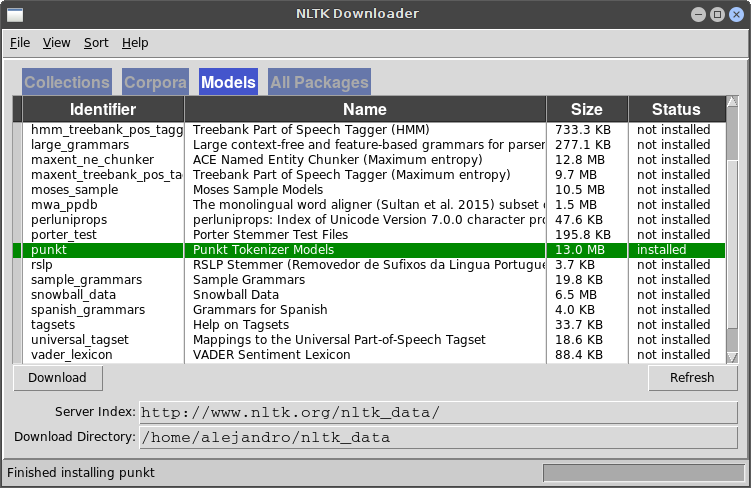
\includegraphics[width=0.8\textwidth]{nltk_download}
\end{center}
\begin{itemize}
	\item Verán una pantalla como esta, aquí está todo el contenido de nltk para descargar.
	\item Vayan a la sección de \textbf{Models} y descarguen \textbf{punkt}, que como verán, son modelos de tokenización.
\end{itemize}
}



\frame{
\frametitle{NLTK}
\framesubtitle{Tokenizador}
\begin{itemize}
	\item Y ahora que ya descargamos el tokenizador, podemos cerrar esa ventana y usarlo. De regreso en Python.
\end{itemize}
\colorbox{source}{\parbox{\textwidth}{
\ttfamily
\small
\mbox{}\\
\textbf{\textcolor{RoyalBlue}{import}}\ nltk \\
\mbox{} \\
\mbox{}carpeta$\_$nombre\textcolor{BrickRed}{=}\texttt{\textcolor{Red}{"{}C:\textbackslash{}\textbackslash{}Users\textbackslash{}\textbackslash{}user\textbackslash{}\textbackslash{}Desktop\textbackslash{}\textbackslash{}Documentos\textbackslash{}\textbackslash{}"{}}} \\
\mbox{}archivo$\_$nombre\textcolor{BrickRed}{=}\texttt{\textcolor{Red}{"{}P$\_$IFT$\_$290216$\_$73$\_$Acc.txt"{}}} \\
\mbox{} \\
\mbox{}with\ \textbf{\textcolor{Black}{open}}\textcolor{BrickRed}{(}carpeta$\_$nombre\textcolor{BrickRed}{+}archivo$\_$nombre\textcolor{BrickRed}{,}\texttt{\textcolor{Red}{"{}r"{}}}\textcolor{BrickRed}{)}\ as\ archivo\textcolor{BrickRed}{:} \\
\mbox{}\ \ \ \ \ \ \ \ texto\textcolor{BrickRed}{=}archivo\textcolor{BrickRed}{.}\textbf{\textcolor{Black}{read}}\textcolor{BrickRed}{()} \\
\mbox{} \\
\mbox{}tokens\textcolor{BrickRed}{=}nltk\textcolor{BrickRed}{.}\textbf{\textcolor{Black}{word$\_$tokenize}}\textcolor{BrickRed}{(}texto\textcolor{BrickRed}{,}\texttt{\textcolor{Red}{"{}spanish"{}}}\textcolor{BrickRed}{)} \\
\mbox{} \\
\mbox{}\textbf{\textcolor{Blue}{for}}\ token\ \textbf{\textcolor{Blue}{in}}\ tokens\textcolor{BrickRed}{:} \\
\mbox{}\ \ \ \ \ \ \ \ \textbf{\textcolor{Blue}{print}}\textcolor{BrickRed}{(}token\textcolor{BrickRed}{)} \\
\mbox{}
}}
}
\note{
\begin{itemize}
	\item Ya sabemos como abrir y leer archivos.
	\item El tokenizdor de NLTK (la función {\tt\textbf{word\_tokenize()}} usa el texto leído y regresa una lista con los tokens que encuentra.
	\item Como es una lista, podemos hacer un bucle para recorrerla y mostrar el resultado.
	\item Notarán algo, estamos dando un segundo parámetro a {\tt\textbf{word\_tokenize()}} para indicar que nuestro texto está en español (de allí que el parámetro es: {\tt{"{spanish}"{}}}).
	\item El tokenizador tiene varios modelos, adaptados para diferentes idiomas, si tienen la curiosidad y el tiempo, pueden entrar a la carpeta en la que se descargó en tokenizador para  que vean los idiomas que sabe manejar. 
\end{itemize}
}
\note{
\begin{itemize}
	\item En cuanto al resultado, pueden comparar los tokens que se obtienen con este método contra los de nuestro pequeño tokenizador de expresiones regulares.
	\item Verán que, por ejemplo, este detecta mejor abreviaciones como "{}{\tt S.A.}"{} ya que el nuestro separa el último punto. Pero este no separa los punto y guión ({\tt.-}) de las palabras que tiene junto, y el nuestro sí.
	\item Las reglas y los procesos que se usan en cada herramienta varían, es importante revisar los resultados que se tienen y escoger la mejor herramienta para cada tarea.
\end{itemize}
}



\frame{
\frametitle{Conteo de palabras}
\framesubtitle{o mejor dicho de tokens}
\small
\begin{itemize}
	\item Así que ahora tenemos dos maneras de obtener una lista de tokens para nuestros textos.
	\item Veamos un par de usos, pueden ocupar la lista que más les guste.
	\item Para empezar, podemos usarlas para contar el total de palabras del documento.
\end{itemize}
\colorbox{source}{\parbox{\textwidth}{
\ttfamily
\mbox{}\\
\textit{\textcolor{Brown}{\#\ Aquí,\ nuestra\ lista\ de\ tokens\ se\ llama\ "{}tokens"{}}} \\
\mbox{} \\
\mbox{}palabras$\_$total\textcolor{BrickRed}{=}\textbf{\textcolor{Black}{len}}\textcolor{BrickRed}{(}tokens\textcolor{BrickRed}{)} \\
\mbox{} \\
\mbox{}\textbf{\textcolor{Blue}{print}}\textcolor{BrickRed}{(}palabras$\_$total\textcolor{BrickRed}{)} \\
\mbox{}
}}
}
\note{
\begin{itemize}
	\item ¿Recuerdan la función {\tt\textbf{len()}} de las listas? Nos proporciona el tamaño de la lista.
	\item Si tomamos en cuenta que la lista de tokens contiene (separados) cada uno de los elementos que tiene el texto, bastará con ver qué longitud tiene para saber cuántos elementos tiene el texto.
	\item Esto va a incluir símbolos y puntuación, tengan eso en mente.
\end{itemize}
}



\frame{
\frametitle{Palabras diferentes}
\small
\begin{itemize}
	\item Además de las palabras totales, nos puede interesar conocer las palabras diferentes que utiliza un texto.
	\item Para esto, podemos utilizar el {\tt\textbf{set}} de Python.
	\item Un {\tt\textbf{set}} es un conjunto. Es similar a una lista pero están pensados para hacer operaciones entre conjuntos (como uniones, intersecciones o diferencias). Y una característica particular que por ahora nos interesa bastante es que sus elementos no se repiten.
	\item Se usa la función {\tt\textbf{set()}} para convertir una lista en un conjunto.
\end{itemize}
\colorbox{source}{\parbox{\textwidth}{
\ttfamily
\mbox{}\\
\textit{\textcolor{Brown}{\#\ Aquí,\ nuestra\ lista\ de\ tokens\ se\ llama\ "{}tokens"{}}} \\
\mbox{} \\
\mbox{}tokens$\_$conjunto\textcolor{BrickRed}{=}\textbf{\textcolor{Black}{set}}\textcolor{BrickRed}{(}tokens\textcolor{BrickRed}{)} \\
\mbox{}palabras$\_$diferentes\textcolor{BrickRed}{=}\textbf{\textcolor{Black}{len}}\textcolor{BrickRed}{(}tokens$\_$conjunto\textcolor{BrickRed}{)} \\
\mbox{} \\
\mbox{}\textbf{\textcolor{Blue}{print}}\textcolor{BrickRed}{(}palabras$\_$diferentes\textcolor{BrickRed}{)} \\
\mbox{}
}}
}




\frame{
\frametitle{Riqueza léxica}
\small
\begin{itemize}
	\item La riqueza léxica es la relación que existe entre la extensión de un texto y el número de palabras distintas que contiene.
	\item Así que ahora es muy fácil para nosotros calcularla.
\end{itemize}
\colorbox{source}{\parbox{\textwidth}{
\ttfamily
\mbox{}\\
\textit{\textcolor{Brown}{\#\ Aquí,\ nuestra\ lista\ de\ tokens\ se\ llama\ "{}tokens"{}}} \\
\mbox{} \\
\mbox{}tokens$\_$conjunto\textcolor{BrickRed}{=}\textbf{\textcolor{Black}{set}}\textcolor{BrickRed}{(}tokens\textcolor{BrickRed}{)} \\
\mbox{} \\
\mbox{}palabras$\_$totales\textcolor{BrickRed}{=}\textbf{\textcolor{Black}{len}}\textcolor{BrickRed}{(}tokens\textcolor{BrickRed}{)} \\
\mbox{}palabras$\_$diferentes\textcolor{BrickRed}{=}\textbf{\textcolor{Black}{len}}\textcolor{BrickRed}{(}tokens$\_$conjunto\textcolor{BrickRed}{)} \\
\mbox{} \\
\mbox{}riqueza$\_$lexica\textcolor{BrickRed}{=}palabras$\_$diferentes\textcolor{BrickRed}{/}palabras$\_$totales \\
\mbox{} \\
\mbox{}\textbf{\textcolor{Blue}{print}}\textcolor{BrickRed}{(}riqueza$\_$lexica\textcolor{BrickRed}{)} \\
\mbox{}
}}
}



\frame{
\frametitle{Funciones}
\framesubtitle{en Python claro}
\small
\begin{itemize}
	\item Hemos visto muchas funciones. Ahora veamos que también podemos crearlas nosotros mismos.
	\item Hagamos una función que calcule la riqueza léxica si le damos una lista de tokens.
\end{itemize}
\colorbox{source}{\parbox{\textwidth}{
\ttfamily
\mbox{}\\
\textbf{\textcolor{Blue}{def}}\ \textbf{\textcolor{Black}{riqueza$\_$lexica}}\textcolor{BrickRed}{(}tokens\textcolor{BrickRed}{):} \\
\mbox{}\ \ \ \ tokens$\_$conjunto\textcolor{BrickRed}{=}\textbf{\textcolor{Black}{set}}\textcolor{BrickRed}{(}tokens\textcolor{BrickRed}{)} \\
\mbox{}\ \ \ \  \\
\mbox{}\ \ \ \ palabras$\_$totales\textcolor{BrickRed}{=}\textbf{\textcolor{Black}{len}}\textcolor{BrickRed}{(}tokens\textcolor{BrickRed}{)} \\
\mbox{}\ \ \ \ palabras$\_$diferentes\textcolor{BrickRed}{=}\textbf{\textcolor{Black}{len}}\textcolor{BrickRed}{(}tokens$\_$conjunto\textcolor{BrickRed}{)} \\
\mbox{}\ \ \ \  \\
\mbox{}\ \ \ \ riqueza$\_$lexica\textcolor{BrickRed}{=}palabras$\_$diferentes\textcolor{BrickRed}{/}palabras$\_$totales \\
\mbox{}\ \ \ \  \\
\mbox{}\ \ \ \ \textbf{\textcolor{Blue}{return}}\ riqueza$\_$lexica \\
\mbox{}
}}
}
\note{
\footnotesize
\vspace{-0.3cm}
\begin{itemize}
	\item Las funciones se crean con la instrucción especial {\tt\textbf{def}} seguido del nombre de la función y los paréntesis (toda función lleva paréntesis) dentro de los que se pueden usar parámetros.
	\item Los parámetros son básicamente variables que se asignan al momento de llamar la función. En el caso del ejemplo, el parámetro {\tt\textbf{tokens}} se puede usar dentro de la función como una variable. Su valor estará dado por lo que se ponga entre los paréntesis en el momento de usar la función (más adelante en el programa).
	\item Las variables dentro de una función son válidas UNICAMENTE DENTRO DE LA FUNCIÓN. Eso quiere decir que si más adelante en el programa, fuera de la función, se intenta usar una de las variables definidas dentro de la función no va a funcionar.
	\item La instrucción {\tt\textbf{return}} es una instrucción especial de las funciones, llegando a ese punto, la función termina y regresa el valor especificado. Esto quiere decir que ese resultado se podrá asignar a una variable más adelante.
\end{itemize}
}




\frame{
\frametitle{Funciones}
\colorbox{source}{\parbox{\textwidth}{
\ttfamily
\footnotesize
\mbox{}\\
\textbf{\textcolor{RoyalBlue}{import}}\ nltk \\
\mbox{} \\
\mbox{}\textbf{\textcolor{Blue}{def}}\ \textbf{\textcolor{Black}{riqueza$\_$lexica}}\textcolor{BrickRed}{(}tokens\textcolor{BrickRed}{):} \\
\mbox{}\ \ \ \ \ \ \ \ tokens$\_$conjunto\textcolor{BrickRed}{=}\textbf{\textcolor{Black}{set}}\textcolor{BrickRed}{(}tokens\textcolor{BrickRed}{)} \\
\mbox{}\ \ \ \ \ \ \ \ palabras$\_$totales\textcolor{BrickRed}{=}\textbf{\textcolor{Black}{len}}\textcolor{BrickRed}{(}tokens\textcolor{BrickRed}{)} \\
\mbox{}\ \ \ \ \ \ \ \ palabras$\_$diferentes\textcolor{BrickRed}{=}\textbf{\textcolor{Black}{len}}\textcolor{BrickRed}{(}tokens$\_$conjunto\textcolor{BrickRed}{)} \\
\mbox{}\ \ \ \ \ \ \ \ riqueza$\_$lexica\textcolor{BrickRed}{=}palabras$\_$diferentes\textcolor{BrickRed}{/}palabras$\_$totales \\
\mbox{}\ \ \ \ \ \ \ \ \textbf{\textcolor{Blue}{return}}\ riqueza$\_$lexica \\
\mbox{} \\
\mbox{}carpeta$\_$nombre\textcolor{BrickRed}{=}\texttt{\textcolor{Red}{"{}C:\textbackslash{}\textbackslash{}Users\textbackslash{}\textbackslash{}user\textbackslash{}\textbackslash{}Desktop\textbackslash{}\textbackslash{}Documentos\textbackslash{}\textbackslash{}"{}}} \\
\mbox{}archivo$\_$nombre\textcolor{BrickRed}{=}\texttt{\textcolor{Red}{"{}P$\_$IFT$\_$290216$\_$73$\_$Acc.txt"{}}} \\
\mbox{} \\
\mbox{}with\ \textbf{\textcolor{Black}{open}}\textcolor{BrickRed}{(}carpeta$\_$nombre\textcolor{BrickRed}{+}archivo$\_$nombre\textcolor{BrickRed}{,}\texttt{\textcolor{Red}{"{}r"{}}}\textcolor{BrickRed}{)}\ as\ archivo\textcolor{BrickRed}{:} \\
\mbox{}\ \ \ \ \ \ \ \ texto\textcolor{BrickRed}{=}archivo\textcolor{BrickRed}{.}\textbf{\textcolor{Black}{read}}\textcolor{BrickRed}{()} \\
\mbox{} \\
\mbox{}tokens\textcolor{BrickRed}{=}nltk\textcolor{BrickRed}{.}\textbf{\textcolor{Black}{word$\_$tokenize}}\textcolor{BrickRed}{(}texto\textcolor{BrickRed}{,}\texttt{\textcolor{Red}{"{}spanish"{}}}\textcolor{BrickRed}{)} \\
\mbox{}riqueza$\_$lexica\textcolor{BrickRed}{=}\textbf{\textcolor{Black}{riqueza$\_$lexica}}\textcolor{BrickRed}{(}tokens\textcolor{BrickRed}{)} \\
\mbox{}\textbf{\textcolor{Blue}{print}}\textcolor{BrickRed}{(}riqueza$\_$lexica\textcolor{BrickRed}{)} \\
\mbox{}
}}
}
\note{
\begin{itemize}
	\item Aquí se muestra un ejemplo más completo.
	\item Noten que las funciones se definen pronto dentro del archivo de Python, esto facilita a que no se pierdan las funciones entre el resto del código, y para que estén disponibles desde el principio. Las funciones SOLO están disponibles DESPUÉS de que fueron definidas.
	\item Como pueden ver, la función se usa más adelante, después de que fue creada, y los nombres de las variables NO AFECTAN a la función. Es decir, la función fue definida con un parámetro de entrada {\tt\textbf{tokens}}, pero eso es solo para la función, fuera de ella, se puede usar el nombre independientemente, es más, como se ve se puede usar el nombre {\tt\textbf{tokens}} para guardar la información que más tarde se le pasa a la función aunque tenga el mismo nombre del parámetro.
\end{itemize}
}
\note{
\begin{itemize}
	\item Otro detalle que ilustra el ejemplo está en los nombres de las funciones. Observen como la función y la variable a la que se asigna el resultado de la función, se llaman igual. Esto es correcto, no pasa nada, ya que la diferencia está en que parte del nombre de la función son los paréntesis, una función se diferenciará de una variable del mismo nombre siempre por los paréntesis.
	\item Además de eso, aquí se puede ver cómo es que el resultado de la función se asigna a una variable, esto es gracias a la instrucción {\tt\textbf{return}} que finaliza la función, el valor que estaba en la variable {\tt\textbf{riqueza\_lexica}} de la función se devuelve luego de ser llamada. Y, en el caso del ejemplo, se guarda en OTRA variable que se llama {\tt\textbf{riqueza\_lexica}}, todo eso ya FUERA de la función.
\end{itemize}
}




\frame{
\frametitle{Ejercicio}
\begin{itemize}
	\item Modificar la función que se creó para que en lugar de recibir una lista de tokens, reciba texto (el texto que se lea de un archivo por ejemplo).
	\item NOTA: Se tendrán que agregar todos los pasos necesarios para que la función trabaje de manera correcta y que devuelva la riqueza léxica del texto que introduzcan.
\end{itemize}
}




\frame{
\frametitle{Conteo individual}
\begin{itemize}
	\item También podemos usar la lista de tokens para hacer conteos de palabras individuales.
	\item Para esto, utilizamos la función {\tt\textbf{count()}} de la lista.
\end{itemize}
\colorbox{source}{\parbox{\textwidth}{
\ttfamily
\mbox{}\\
\textit{\textcolor{Brown}{\#\ Aquí,\ nuestra\ lista\ de\ tokens\ se\ llama\ "{}tokens"{}}} \\
\mbox{} \\
\mbox{}conteo$\_$individual\textcolor{BrickRed}{=}tokens\textcolor{BrickRed}{.}\textbf{\textcolor{Black}{count}}\textcolor{BrickRed}{(}\texttt{\textcolor{Red}{"{}el"{}}}\textcolor{BrickRed}{)} \\
\mbox{} \\
\textbf{\textcolor{Blue}{print}}\textcolor{BrickRed}{(}conteo$\_$individual\textcolor{BrickRed}{)} \\
\mbox{}
\mbox{} \\
\mbox{}palabras$\_$totales\textcolor{BrickRed}{=}\textbf{\textcolor{Black}{len}}\textcolor{BrickRed}{(}tokens\textcolor{BrickRed}{)} \\
\mbox{}porcentaje\textcolor{BrickRed}{=}\textcolor{Purple}{100}\textcolor{BrickRed}{*}conteo$\_$individual\textcolor{BrickRed}{/}palabras$\_$totales \\
\mbox{} \\
\mbox{}\textbf{\textcolor{Blue}{print}}\textcolor{BrickRed}{(}porcentaje\textcolor{BrickRed}{,}\texttt{\textcolor{Red}{"{}\%"{}}}\textcolor{BrickRed}{)} \\
\mbox{}
}}
}




\frame{
\frametitle{Funciones}
\small
\begin{itemize}
	\item Algunas funciones reciben más de un dato. Cuando esto pasa se separan por comas dentro de los paréntesis.
	\item Cuando definimos funciones, también podemos definir más de un parámetro de entrada. De igual manera, separados por comas.
\end{itemize}
\colorbox{source}{\parbox{\textwidth}{
\ttfamily
\small
\mbox{}\\
\textbf{\textcolor{Blue}{def}}\ \textbf{\textcolor{Black}{porcentaje}}\textcolor{BrickRed}{(}palabra\textcolor{BrickRed}{,}texto\textcolor{BrickRed}{):} \\
\mbox{}\ \ \ \ \textit{\textcolor{Brown}{\#\ Aquí\ va\ el\ programa}} \\
\mbox{}\ \ \ \ \textit{\textcolor{Brown}{\#\ Se\ pueden\ usar\ las\ variables\ "{}palabra"{}\ y\ "{}texto"{}}} \\
\mbox{}\ \ \ \ \textit{\textcolor{Brown}{\#\ al\ momento\ de\ usar\ la\ función,\ los\ parámetros\ se}} \\
\mbox{}\ \ \ \ \textit{\textcolor{Brown}{\#\ \ \ asignan\ por\ el\ orden.\ Es\ decir,\ el\ primero}} \\
\mbox{}\ \ \ \ \textit{\textcolor{Brown}{\#\ \ \ parámetro\ será\ "{}palabra"{},\ el\ segundo\ "{}texto"{}.}} \\
\mbox{}\ \ \ \ \textit{\textcolor{Brown}{\#\ Pueden\ definir\ los\ parametros\ como\ quieran}} \\
\mbox{}\ \ \ \ \textit{\textcolor{Brown}{\#\ Solo\ asegurense\ de\ poner\ el\ orden\ correcto\ de\ los}} \\
\mbox{}\ \ \ \ \textit{\textcolor{Brown}{\#\ \ \ datos\ al\ momento\ de\ usar\ su\ función}} \\
\mbox{}
}}
}




\frame{
\frametitle{Ejercicio}
Para que quede bien claro el uso de funciones
\begin{itemize}
	\item Definir una función que calcule el porcentaje que ocupa una palabra dentro de un textos. Usen como parámetros de entrada la palabra y el texto.
\end{itemize}
}




\frame{
\frametitle{NLTK}
\begin{itemize}
	\item De regreso a NLTK, también podemos usar los tokens para crear una variable de tipo {\tt\textbf{Text}} de NLTK.
	\item Estos objetos tienen varias funciones útiles.
\end{itemize}
\colorbox{source}{\parbox{\textwidth}{
\ttfamily
\small
\mbox{}\\
\textbf{\textcolor{RoyalBlue}{import}}\ nltk \\
\mbox{} \\
\mbox{}carpeta$\_$nombre\textcolor{BrickRed}{=}\texttt{\textcolor{Red}{"{}C:\textbackslash{}\textbackslash{}Users\textbackslash{}\textbackslash{}user\textbackslash{}\textbackslash{}Desktop\textbackslash{}\textbackslash{}Documentos\textbackslash{}\textbackslash{}"{}}} \\
\mbox{}archivo$\_$nombre\textcolor{BrickRed}{=}\texttt{\textcolor{Red}{"{}P$\_$IFT$\_$290216$\_$73$\_$Acc.txt"{}}} \\
\mbox{} \\
\mbox{}with\ \textbf{\textcolor{Black}{open}}\textcolor{BrickRed}{(}carpeta$\_$nombre\textcolor{BrickRed}{+}archivo$\_$nombre\textcolor{BrickRed}{,}\texttt{\textcolor{Red}{"{}r"{}}}\textcolor{BrickRed}{)}\ as\ archivo\textcolor{BrickRed}{:} \\
\mbox{}\ \ \ \ \ \ \ \ texto\textcolor{BrickRed}{=}archivo\textcolor{BrickRed}{.}\textbf{\textcolor{Black}{read}}\textcolor{BrickRed}{()} \\
\mbox{} \\
\mbox{}tokens\textcolor{BrickRed}{=}nltk\textcolor{BrickRed}{.}\textbf{\textcolor{Black}{word$\_$tokenize}}\textcolor{BrickRed}{(}texto\textcolor{BrickRed}{,}\texttt{\textcolor{Red}{"{}spanish"{}}}\textcolor{BrickRed}{)} \\
\mbox{} \\
\mbox{}texto$\_$nltk\textcolor{BrickRed}{=}nltk\textcolor{BrickRed}{.}\textbf{\textcolor{Black}{Text}}\textcolor{BrickRed}{(}tokens\textcolor{BrickRed}{)} \\
\mbox{}
}}
}
\note{
\begin{itemize}
	\item Las variables tipo {\tt\textbf{Text}} de NLTK muchas veces también se comportan como listas.
	\item Por ejemplo, pueden usar su función {\tt\textbf{count()}} para ver las repeticiones de una palabra, y pueden también usar la función {\tt\textbf{len()}} para ver la longitud total de palabras o la función {\tt\textbf{set()}} para convertirla en un conjunto.
\end{itemize}
}



\frame{
\frametitle{NLTK}
\framesubtitle{Concordancias}
\small
\vspace{-0.5cm}
\begin{itemize}
	\item Las concordacias muestran todas las apariciones de una palabra junto con algo del texto que la rodea.
	\item Con la función {\tt\textbf{concordance()}} de el {\tt\textbf{Text}} de NLTK es mostrar las concordancias de una palabra.
\end{itemize}
\colorbox{source}{\parbox{\textwidth}{
\footnotesize
\small
\mbox{}\\
\textbf{\textcolor{RoyalBlue}{import}}\ nltk \\
\mbox{} \\
\mbox{}carpeta$\_$nombre\textcolor{BrickRed}{=}\texttt{\textcolor{Red}{"{}C:\textbackslash{}\textbackslash{}Users\textbackslash{}\textbackslash{}user\textbackslash{}\textbackslash{}Desktop\textbackslash{}\textbackslash{}Documentos\textbackslash{}\textbackslash{}"{}}} \\
\mbox{}archivo$\_$nombre\textcolor{BrickRed}{=}\texttt{\textcolor{Red}{"{}P$\_$IFT$\_$290216$\_$73$\_$Acc.txt"{}}} \\
\mbox{} \\
\mbox{}with\ \textbf{\textcolor{Black}{open}}\textcolor{BrickRed}{(}carpeta$\_$nombre\textcolor{BrickRed}{+}archivo$\_$nombre\textcolor{BrickRed}{,}\texttt{\textcolor{Red}{"{}r"{}}}\textcolor{BrickRed}{)}\ as\ archivo\textcolor{BrickRed}{:} \\
\mbox{}\ \ \ \ \ \ \ \ texto\textcolor{BrickRed}{=}archivo\textcolor{BrickRed}{.}\textbf{\textcolor{Black}{read}}\textcolor{BrickRed}{()} \\
\mbox{} \\
\mbox{}tokens\textcolor{BrickRed}{=}nltk\textcolor{BrickRed}{.}\textbf{\textcolor{Black}{word$\_$tokenize}}\textcolor{BrickRed}{(}texto\textcolor{BrickRed}{,}\texttt{\textcolor{Red}{"{}spanish"{}}}\textcolor{BrickRed}{)} \\
\mbox{} \\
\mbox{}texto$\_$nltk\textcolor{BrickRed}{=}nltk\textcolor{BrickRed}{.}\textbf{\textcolor{Black}{Text}}\textcolor{BrickRed}{(}tokens\textcolor{BrickRed}{)} \\
\mbox{}texto$\_$nltk\textcolor{BrickRed}{.}\textbf{\textcolor{Black}{concordance}}\textcolor{BrickRed}{(}\texttt{\textcolor{Red}{"{}artículo"{}}}\textcolor{BrickRed}{)} \\
\mbox{}
}}
}
\note{
\begin{itemize}
	\item Es importante notar, que las concordancias de NLTK buscan según los tokens SIN importar mayúsculas y minúsculas, pero sí la coincidencia completa de la palabra.
	\item Esto quiere decir, que el ejemplo sería capaz de encontrar la palabra "{}Artículo"{} si la hubiera, pero no "{}artículos"{} aunque la haya.
	\item Pueden probar buscando la palabra "{}ley"{} para ver que las mayúsculas y minúsculas se buscan por igual.
	\item Otro detalle, la función {\tt\textbf{concordance()}} es similar a la función {\tt\textbf{print()}} en cuanto a que su propósito es mostrar ese resultado en pantalla, NO funciona para mandar el resultado a una variable.
\end{itemize}
}



\frame{
\frametitle{RE}
\framesubtitle{Concordancias}
\small
\vspace{-0.5cm}
\begin{itemize}
	\item Aprovecharé este punto para explicar un símbolo de las expresiones regulares que no había mencionado. Los corchetes: {\tt\textbf{\{\}}}
	\item Y para mostrarles cómo hacer concordancias con RE, por si quieren ampliar su funcionamiento o simplemente no cargar nltk.
\end{itemize}
\colorbox{source}{\parbox{\textwidth}{
\footnotesize
\small
\mbox{}\\
\textbf{\textcolor{RoyalBlue}{import}}\ re \\
\mbox{} \\
\mbox{}\textit{\textcolor{Brown}{\#\ Aqui\ va\ la\ lectura\ del\ archivo,\ por\ ahora\ la\ estoy\ omitiendo}} \\
\mbox{} \\
\mbox{}expresion\textcolor{BrickRed}{=}re\textcolor{BrickRed}{.}\textbf{\textcolor{Black}{compile}}\textcolor{BrickRed}{(}r\texttt{\textcolor{Red}{"{}.\{,30\}[\textbackslash{}s\textasciicircum{}][Aa]rtículos?\ .\{,30\}"{}}}\textcolor{BrickRed}{)} \\
\mbox{}resultados$\_$busqueda\textcolor{BrickRed}{=}expresion\textcolor{BrickRed}{.}\textbf{\textcolor{Black}{finditer}}\textcolor{BrickRed}{(}texto\textcolor{BrickRed}{)} \\
\mbox{} \\
\mbox{}\textbf{\textcolor{Blue}{for}}\ resultado\ \textbf{\textcolor{Blue}{in}}\ resultados$\_$busqueda\textcolor{BrickRed}{:} \\
\mbox{}\ \ \ \ \ \ \ \ \textbf{\textcolor{Blue}{print}}\textcolor{BrickRed}{(}resultado\textcolor{BrickRed}{.}\textbf{\textcolor{Black}{group}}\textcolor{BrickRed}{(}\textcolor{Purple}{0}\textcolor{BrickRed}{))} \\
\mbox{}
}}
}
\note{
\vspace{-0.3cm}
\footnotesize
\begin{itemize}
	\item Los corchetes sirven para especificar un número concreto de repeticiones del símbolo que les precede. Esto quiere decir que si tenemos, por ejemplo: {\tt\textbf{.\{3\}}} Quiere decir que se buscan 3 letras, las que sean.
	\item Además de eso, el corchete puede usarse para rangos delimitados de repeticiones. Esto quiere decir que podemos buscar, por ejemplo, entre 2 y 6 caracteres: {\tt\textbf{.\{2,6\}}}.
	\item Si se omite uno de esos dos números, quiere decir que no hay límite, como en el ejemplo, que se busca de cero (por eso no hay número, es igual si se pone 0) hasta 30 caracteres en ambos lados de la palabra.
	\item Con las expresiones regulares se tienen que tomar en cuenta más cosas para lograr una buena concordancia, pero de igual manera, se pueden lograr mas cosas, en este ejemplo, estamos incluyendo, por ejemplo, que la palabra pueda aparecer al inicio de la línea, que pueda aparecer con mayúscula en la primera letra, o que pueda contener una s al final. Las primeras dos funciones las cumplen las concordancias de NLTK, la tercera no. Una vez más, depende del objetivo, la herramienta que se debe usar.
\end{itemize}
}



\frame{
\frametitle{NLTK}
\framesubtitle{Palabras similares}
\small
\begin{itemize}
	\item De nuevo en NLTK, veamos otra de las funciones que tiene sus {\tt\textbf{Text}}.
	\item Hemos visto que la función {\tt\textbf{concordance()}} nos muestra una palabra en su contexto.
	\item Pero también tiene la función {\tt\textbf{similar()}} que es capaz de mostrarnos otras palabras, que tengan contextos similares.
\end{itemize}
\colorbox{source}{\parbox{\textwidth}{
\footnotesize
\small
\mbox{}\\
\textbf{\textcolor{RoyalBlue}{import}}\ nltk \\
\mbox{} \\
\mbox{}\textit{\textcolor{Brown}{\#\ Aqui\ va\ la\ lectura\ del\ archivo,\ por\ ahora\ la\ estoy\ omitiendo}} \\
\mbox{} \\
\mbox{}tokens\textcolor{BrickRed}{=}nltk\textcolor{BrickRed}{.}\textbf{\textcolor{Black}{word$\_$tokenize}}\textcolor{BrickRed}{(}texto\textcolor{BrickRed}{,}\texttt{\textcolor{Red}{"{}spanish"{}}}\textcolor{BrickRed}{)} \\
\mbox{} \\
\mbox{}texto$\_$nltk\textcolor{BrickRed}{=}nltk\textcolor{BrickRed}{.}\textbf{\textcolor{Black}{Text}}\textcolor{BrickRed}{(}tokens\textcolor{BrickRed}{)} \\
\mbox{}texto$\_$nltk\textcolor{BrickRed}{.}\textbf{\textcolor{Black}{similar}}\textcolor{BrickRed}{(}\texttt{\textcolor{Red}{"{}artículo"{}}}\textcolor{BrickRed}{)} \\
\mbox{}
}}
}



\frame{
\frametitle{NLTK}
\framesubtitle{Palabras similares}
\vspace{-0.4cm}
\small
\begin{itemize}
	\item Para este tipo de funciones, entre más texto se tenga para hacer el análisis es mejor.
	\item Hasta ahora, hemos usado un texto corto para los ejemplos, probemos ahora con el conjunto de todos los que tenemos.
\end{itemize}
\colorbox{source}{\parbox{\textwidth}{
\footnotesize
\mbox{}\\
\textbf{\textcolor{RoyalBlue}{import}}\ nltk \\
\mbox{} \\
\mbox{}carpeta$\_$nombre\textcolor{BrickRed}{=}\texttt{\textcolor{Red}{"{}C:\textbackslash{}\textbackslash{}Users\textbackslash{}\textbackslash{}user\textbackslash{}\textbackslash{}Desktop\textbackslash{}\textbackslash{}Documentos\textbackslash{}\textbackslash{}"{}}} \\
\mbox{}archivo$\_$nombre\textcolor{BrickRed}{=}\texttt{\textcolor{Red}{"{}DOF\_P\_IFT\_291116\_672\_Acc.txt"{}}} \\
\mbox{} \\
\mbox{} \\
\mbox{}with\ \textbf{\textcolor{Black}{open}}\textcolor{BrickRed}{(}carpeta$\_$nombre\textcolor{BrickRed}{+}archivo$\_$nombre\textcolor{BrickRed}{,}\texttt{\textcolor{Red}{"{}r"{}}}\textcolor{BrickRed}{)}\ as\ archivo\textcolor{BrickRed}{:} \\
\mbox{}\ \ \ \ \ \ \ \ texto\textcolor{BrickRed}{=}archivo\textcolor{BrickRed}{.}\textbf{\textcolor{Black}{read}}\textcolor{BrickRed}{()} \\
\mbox{} \\
\mbox{}tokens\textcolor{BrickRed}{=}nltk\textcolor{BrickRed}{.}\textbf{\textcolor{Black}{word$\_$tokenize}}\textcolor{BrickRed}{(}texto\textcolor{BrickRed}{,}\texttt{\textcolor{Red}{"{}spanish"{}}}\textcolor{BrickRed}{)} \\
\mbox{} \\
\mbox{}texto$\_$nltk\textcolor{BrickRed}{=}nltk\textcolor{BrickRed}{.}\textbf{\textcolor{Black}{Text}}\textcolor{BrickRed}{(}tokens\textcolor{BrickRed}{)} \\
\mbox{}texto$\_$nltk\textcolor{BrickRed}{.}\textbf{\textcolor{Black}{similar}}\textcolor{BrickRed}{(}\texttt{\textcolor{Red}{"{}artículo"{}}}\textcolor{BrickRed}{)} \\
\mbox{}
}}
}



\frame{
\frametitle{NLTK}
\framesubtitle{Contextos comunes}
\begin{itemize}
	\item Por supuesto, podemos ver cuál es el contexto que comparten las palabras similares.
\end{itemize}
\colorbox{source}{\parbox{\textwidth}{
\mbox{} \\
\mbox{}tokens\textcolor{BrickRed}{=}nltk\textcolor{BrickRed}{.}\textbf{\textcolor{Black}{word$\_$tokenize}}\textcolor{BrickRed}{(}texto\textcolor{BrickRed}{,}\texttt{\textcolor{Red}{"{}spanish"{}}}\textcolor{BrickRed}{)} \\
\mbox{} \\
\mbox{}texto$\_$nltk\textcolor{BrickRed}{=}nltk\textcolor{BrickRed}{.}\textbf{\textcolor{Black}{Text}}\textcolor{BrickRed}{(}tokens\textcolor{BrickRed}{)} \\
\mbox{}texto$\_$nltk\textcolor{BrickRed}{.}\textbf{\textcolor{Black}{similar}}\textcolor{BrickRed}{(}\texttt{\textcolor{Red}{"{}artículo"{}}}\textcolor{BrickRed}{)} \\
\mbox{}\textbf{\textcolor{Blue}{print}}\textcolor{BrickRed}{()} \\
\mbox{}texto$\_$nltk\textcolor{BrickRed}{.}\textbf{\textcolor{Black}{common$\_$contexts}}\textcolor{BrickRed}{([}\texttt{\textcolor{Red}{"{}artículo"{}}}\textcolor{BrickRed}{,}\texttt{\textcolor{Red}{"{}instituto"{}}}\textcolor{BrickRed}{])} \\
\mbox{}
}}
\begin{itemize}
	\item La función {\tt\textbf{print()}} es para separar los resultados y sea más claro el contenido de cada parte.
\end{itemize}
}




\frame{
\frametitle{NLTK}
\framesubtitle{Dispersión}
\begin{itemize}
	\item Otra función muy interesante es {\tt\textbf{dispersion\_plot()}}.
	\item Esta función muestra una gráfica con la aparición de una lista de palabras buscadas a lo largo de todo el texto.
\end{itemize}
\colorbox{source}{\parbox{\textwidth}{
\mbox{} \\
tokens\textcolor{BrickRed}{=}nltk\textcolor{BrickRed}{.}\textbf{\textcolor{Black}{word$\_$tokenize}}\textcolor{BrickRed}{(}texto\textcolor{BrickRed}{,}\texttt{\textcolor{Red}{"{}spanish"{}}}\textcolor{BrickRed}{)} \\
\mbox{}texto$\_$nltk\textcolor{BrickRed}{=}nltk\textcolor{BrickRed}{.}\textbf{\textcolor{Black}{Text}}\textcolor{BrickRed}{(}tokens\textcolor{BrickRed}{)} \\
\mbox{} \\
\mbox{}lista$\_$palabras\textcolor{BrickRed}{=[}\texttt{\textcolor{Red}{"{}Instituto"{}}}\textcolor{BrickRed}{,}\texttt{\textcolor{Red}{"{}Ley"{}}}\textcolor{BrickRed}{,}\texttt{\textcolor{Red}{"{}Elija"{}}}\textcolor{BrickRed}{,}\texttt{\textcolor{Red}{"{}ley"{}}}\textcolor{BrickRed}{]} \\
\mbox{}texto$\_$nltk\textcolor{BrickRed}{.}\textbf{\textcolor{Black}{dispersion$\_$plot}}\textcolor{BrickRed}{(}lista$\_$palabras\textcolor{BrickRed}{)} \\
\mbox{}
}}
}
\note{
\begin{itemize}
	\item Una pequeña nota, observen que a diferencia de las otras funciones que hemos visto, aquí SI importa el uso de mayúsculas.
	\item Para esta función, es necesario que tengan instalados los paquetes de python {\tt\textbf{numpy}} y {\tt\textbf{matplotlib}}. Si instalaron Anaconda, seguramente ya cuentan con ambos.
\end{itemize}
}



\frame{
\frametitle{NLTK}
\framesubtitle{Distribución de frecuencias}
\small
\colorbox{source}{\parbox{\textwidth}{
\mbox{} \\
\textbf{\textcolor{RoyalBlue}{import}}\ nltk \\
\mbox{} \\
\mbox{}carpeta$\_$nombre\textcolor{BrickRed}{=}\texttt{\textcolor{Red}{"{}C:\textbackslash{}\textbackslash{}Users\textbackslash{}\textbackslash{}user\textbackslash{}\textbackslash{}Desktop\textbackslash{}\textbackslash{}Documentos\textbackslash{}\textbackslash{}"{}}} \\
\mbox{}archivo$\_$nombre\textcolor{BrickRed}{=}\texttt{\textcolor{Red}{"{}P$\_$IFT$\_$290216$\_$73$\_$Acc.txt"{}}} \\
\mbox{} \\
\mbox{}with\ \textbf{\textcolor{Black}{open}}\textcolor{BrickRed}{(}carpeta$\_$nombre\textcolor{BrickRed}{+}archivo$\_$nombre\textcolor{BrickRed}{,}\texttt{\textcolor{Red}{"{}r"{}}}\textcolor{BrickRed}{)}\ as\ archivo\textcolor{BrickRed}{:} \\
\mbox{}\ \ \ \ \ \ \ \ texto\textcolor{BrickRed}{=}archivo\textcolor{BrickRed}{.}\textbf{\textcolor{Black}{read}}\textcolor{BrickRed}{()} \\
\mbox{} \\
\mbox{}tokens\textcolor{BrickRed}{=}nltk\textcolor{BrickRed}{.}\textbf{\textcolor{Black}{word$\_$tokenize}}\textcolor{BrickRed}{(}texto\textcolor{BrickRed}{,}\texttt{\textcolor{Red}{"{}spanish"{}}}\textcolor{BrickRed}{)} \\
\mbox{} \\
\mbox{}texto$\_$nltk\textcolor{BrickRed}{=}nltk\textcolor{BrickRed}{.}\textbf{\textcolor{Black}{Text}}\textcolor{BrickRed}{(}tokens\textcolor{BrickRed}{)} \\
\mbox{} \\
\mbox{}distribucion\textcolor{BrickRed}{=}nltk\textcolor{BrickRed}{.}\textbf{\textcolor{Black}{FreqDist}}\textcolor{BrickRed}{(}texto$\_$nltk\textcolor{BrickRed}{)} \\
\mbox{} \\
\mbox{}lista$\_$frecuencias\textcolor{BrickRed}{=}distribucion\textcolor{BrickRed}{.}\textbf{\textcolor{Black}{most$\_$common}}\textcolor{BrickRed}{()} \\
\mbox{}\textbf{\textcolor{Blue}{print}}\textcolor{BrickRed}{(}lista$\_$frecuencias\textcolor{BrickRed}{)} \\
\mbox{}
}}
}
\note{
\vspace{-0.35cm}
\small
\begin{itemize}
	\item Hemos visto cómo hacer conteos de palabras totales y de palabras únicas.
	\item Ahora veremos cómo hacer conteos para todas las palabras de un texto. Y para lograrlo podemos usar la función {\tt\textbf{FreqDist()}} de NLTK.
	\item Como ven, usamos la función sobre nuestro {\tt\textbf{Text}} para obtener una distribución.
	\item La distribución tiene su propia función para mostrar la información. La función {\tt\textbf{most\_common()}} que devuelve una lista con cada palabra y su frecuencia. Tal como se puede ver al mostrar la lista que se obtiene con la función {\tt\textbf{print()}}.
	\item La función {\tt\textbf{most\_common()}}, además, puede recibir dentro de los paréntesis un parámetro numérico, el cual indica la cantidad de cuántas palabras queremos que se obtengan en la lista de salida (las más comunes, claro).
\end{itemize}
}




\frame{
\frametitle{NLTK}
\framesubtitle{Distribución de frecuencias}
\small
\begin{itemize}
	\item De la distribución de frecuencias también podemos obtener la frecuencia de una palabra en particular.
	\item Como podrán ver, esto se logra de manera similar a los índices de una lista, pero en lugar de el índice (el número que indica la posición dentro de la lista) se usa la palabra misma, como texto.
\end{itemize}
\colorbox{source}{\parbox{\textwidth}{
\mbox{} \\
\mbox{}\textit{\textcolor{Brown}{\#\ A\ esta\ altura\ ya\ tenemos\ la\ lista\ de\ tokens\ en\ "{}tokens"{}}} \\
\mbox{} \\
\mbox{}texto$\_$nltk\textcolor{BrickRed}{=}nltk\textcolor{BrickRed}{.}\textbf{\textcolor{Black}{Text}}\textcolor{BrickRed}{(}tokens\textcolor{BrickRed}{)} \\
\mbox{} \\
\mbox{}distribucion\textcolor{BrickRed}{=}nltk\textcolor{BrickRed}{.}\textbf{\textcolor{Black}{FreqDist}}\textcolor{BrickRed}{(}texto$\_$nltk\textcolor{BrickRed}{)} \\
\mbox{} \\
\mbox{}\textbf{\textcolor{Blue}{print}}\textcolor{BrickRed}{(}distribucion\textcolor{BrickRed}{[}\texttt{\textcolor{Red}{"{}Instituto"{}}}\textcolor{BrickRed}{])} \\
\mbox{}
}}
}



\frame{
\frametitle{Diccionarios}
\framesubtitle{en Python}
\begin{itemize}
	\item Esas "{}listas"{} que en lugar de usar índices usan palabras, se llaman diccionarios. Es otra herramienta que tiene Python.
	\item OJO, el resultado de la función {\tt\textbf{FreqDist()}} de NLTK en realidad no es un diccionario, ya que tiene funciones propias de NLTK; pero se comporta como un diccionario para obtener su contenido usando palabras.
\end{itemize}
\colorbox{source}{\parbox{\textwidth}{
\mbox{} \\
info\textcolor{BrickRed}{=\{}\texttt{\textcolor{Red}{"{}nombre"{}}}\textcolor{BrickRed}{:}\texttt{\textcolor{Red}{"{}Mi\ nombre"{}}}\textcolor{BrickRed}{,}\texttt{\textcolor{Red}{"{}apellido"{}}}\textcolor{BrickRed}{:}\texttt{\textcolor{Red}{"{}Mi\ apellido"{}}}\textcolor{BrickRed}{\}} \\
\mbox{}info\textcolor{BrickRed}{[}\texttt{\textcolor{Red}{"{}edad"{}}}\textcolor{BrickRed}{]=}\textcolor{Purple}{100} \\
\mbox{}info\textcolor{BrickRed}{[}\texttt{\textcolor{Red}{"{}curso"{}}}\textcolor{BrickRed}{]=}\texttt{\textcolor{Red}{"{}Python"{}}} \\
\mbox{} \\
\mbox{}\textbf{\textcolor{Blue}{for}}\ dato\ \textbf{\textcolor{Blue}{in}}\ info\textcolor{BrickRed}{:} \\
\mbox{}\ \ \ \ \ \ \ \ \textbf{\textcolor{Blue}{print}}\textcolor{BrickRed}{(}dato\textcolor{BrickRed}{,}\texttt{\textcolor{Red}{"{}:"{}}}\textcolor{BrickRed}{,}info\textcolor{BrickRed}{[}dato\textcolor{BrickRed}{])} \\
\mbox{}
}}
}
\note{
\begin{itemize}
	\item Para definir un diccionario, se usan llaves ({\tt\{\}}) en lugar de corchetes ({\tt[]}). Los elementos TAMBIÉN se separan por comas, además, el nombre del dato y el contenido del dato, se separan con dos puntos.
	\item Las funciones que vimos que operan sobre listas (como {\tt\textbf{del()}} y {\tt\textbf{len()}}) también funcionan con diccionarios.
\end{itemize}
}




\frame{
\frametitle{NLTK}
\framesubtitle{Gráfica de frecuencias}
\small
\begin{itemize}
	\item Muchas veces nos interesa observar de una manera visual cómo cambia la frecuencia de las palabras.
	\item Las distribuciones de NLTK tienen opciones para obtener gráficas.
\end{itemize}
\colorbox{source}{\parbox{\textwidth}{
\mbox{} \\
\mbox{}\textit{\textcolor{Brown}{\#\ A\ esta\ altura\ ya\ tenemos\ la\ lista\ de\ tokens\ en\ "{}tokens"{}}} \\
\mbox{} \\
\mbox{}texto$\_$nltk\textcolor{BrickRed}{=}nltk\textcolor{BrickRed}{.}\textbf{\textcolor{Black}{Text}}\textcolor{BrickRed}{(}tokens\textcolor{BrickRed}{)} \\
\mbox{}distribucion\textcolor{BrickRed}{=}nltk\textcolor{BrickRed}{.}\textbf{\textcolor{Black}{FreqDist}}\textcolor{BrickRed}{(}texto$\_$nltk\textcolor{BrickRed}{)} \\
\mbox{} \\
\mbox{}distribucion\textcolor{BrickRed}{.}\textbf{\textcolor{Black}{plot}}\textcolor{BrickRed}{()} \\
\mbox{}
}}
}



\frame{
\frametitle{NLTK}
\framesubtitle{Gráfica de frecuencias}
\small
\begin{itemize}
	\item Seguramente su gráfica muestra demasiadas palabras como para que se entienda claramente el valor de cada una.
	\item Se puede disminuir el número de palabras que se muestran, pueden dar el número que desean como parámetro a la función.
\end{itemize}
\colorbox{source}{\parbox{\textwidth}{
\mbox{} \\
\mbox{}\textit{\textcolor{Brown}{\#\ A\ esta\ altura\ ya\ tenemos\ la\ lista\ de\ tokens\ en\ "{}tokens"{}}} \\
\mbox{} \\
\mbox{}texto$\_$nltk\textcolor{BrickRed}{=}nltk\textcolor{BrickRed}{.}\textbf{\textcolor{Black}{Text}}\textcolor{BrickRed}{(}tokens\textcolor{BrickRed}{)} \\
\mbox{}distribucion\textcolor{BrickRed}{=}nltk\textcolor{BrickRed}{.}\textbf{\textcolor{Black}{FreqDist}}\textcolor{BrickRed}{(}texto$\_$nltk\textcolor{BrickRed}{)} \\
\mbox{} \\
\mbox{}distribucion\textcolor{BrickRed}{.}\textbf{\textcolor{Black}{plot}}\textcolor{BrickRed}{(}\textcolor{Purple}{40}\textcolor{BrickRed}{)} \\
\mbox{}
}}
}




\frame{
\frametitle{NLTK}
\framesubtitle{Gráfica de frecuencias}
\small
\begin{itemize}
	\item Una nota, es probable que su gráfica muestre las palabras cortadas en el eje horizontal.
	\item Esto se puede corregir si agregan las siguientes líneas en algún punto ANTERIOR a usar la gráfica:
\end{itemize}
\colorbox{source}{\parbox{\textwidth}{
\mbox{} \\
\mbox{}\textbf{\textcolor{RoyalBlue}{from}}\ matplotlib\ \textbf{\textcolor{RoyalBlue}{import}}\ rcParams \\
\mbox{}rcParams\textcolor{BrickRed}{.}\textbf{\textcolor{Black}{update}}\textcolor{BrickRed}{(\{}\texttt{\textcolor{Red}{"{}figure.autolayout"{}}}\textcolor{BrickRed}{:}\ True\textcolor{BrickRed}{\})} \\
\mbox{}
}}
\begin{itemize}
	\item No se preocupen mucho por este código, son líneas especiales de configuración de las gráficas.
\end{itemize}
}




\frame{
\frametitle{NLTK}
\framesubtitle{Hapaxes}
\small
\begin{itemize}
	\item Las distribuciones de NLTK también cuentan con una función que regresa los \emph{hapaxes} de un texto. Para ello usamos la función {\tt\textbf{hapaxes()}} de la distribución, y obtenemos una lista con las palabras.
	\item Un \emph{hapax} es una palabra que aparece únicamente una vez en el texto.
\end{itemize}
\colorbox{source}{\parbox{\textwidth}{
\mbox{} \\
\textit{\textcolor{Brown}{\#\ A\ esta\ altura\ ya\ tenemos\ la\ lista\ de\ tokens\ en\ "{}tokens"{}}} \\
\mbox{} \\
\mbox{}texto$\_$nltk\textcolor{BrickRed}{=}nltk\textcolor{BrickRed}{.}\textbf{\textcolor{Black}{Text}}\textcolor{BrickRed}{(}tokens\textcolor{BrickRed}{)} \\
\mbox{}distribucion\textcolor{BrickRed}{=}nltk\textcolor{BrickRed}{.}\textbf{\textcolor{Black}{FreqDist}}\textcolor{BrickRed}{(}texto$\_$nltk\textcolor{BrickRed}{)} \\
\mbox{}hapaxes\textcolor{BrickRed}{=}distribucion\textcolor{BrickRed}{.}\textbf{\textcolor{Black}{hapaxes}}\textcolor{BrickRed}{()} \\
\mbox{} \\
\mbox{}\textbf{\textcolor{Blue}{for}}\ hapax\ \textbf{\textcolor{Blue}{in}}\ hapaxes\textcolor{BrickRed}{:} \\
\mbox{}\ \ \ \ \ \ \ \ \textbf{\textcolor{Blue}{print}}\textcolor{BrickRed}{(}hapax\textcolor{BrickRed}{)} \\
\mbox{}
}}
}



\frame{
\frametitle{NLTK}
\framesubtitle{Gráfica acumulativa de frecuencias}
\small
\begin{itemize}
	\item La gráfica de la distribución tiene un parámetro opcional para transformar la gráfica ene una acumulativa.
	\item Verán que es un parámetro raro, ya que es como poner y asignar una variable dentro de los paréntesis, y básicamente es eso justamente lo que se hace. Ese parámetro no tiene lugar fijo, como se puede ver en el ejemplo.
	\item Además notarán que se usa la palabra especial {\tt\textbf{True}}, que es, como su nombre lo dice, el valor "{}verdadero"{}. Este valor se utiliza para cuando se quiere valores binarios (como cuando se revisa un {\tt\textbf{if}}), también existe el valor {\tt\textbf{False}}.
\end{itemize}
\colorbox{source}{\parbox{\textwidth}{
\mbox{} \\
\mbox{}distribucion\textcolor{BrickRed}{.}\textbf{\textcolor{Black}{plot}}\textcolor{BrickRed}{(}cumulative\textcolor{BrickRed}{=}True\textcolor{BrickRed}{)} \\
\mbox{}distribucion\textcolor{BrickRed}{.}\textbf{\textcolor{Black}{plot}}\textcolor{BrickRed}{(}\textcolor{Purple}{40}\textcolor{BrickRed}{,}cumulative\textcolor{BrickRed}{=}True\textcolor{BrickRed}{)} \\
\mbox{}
}}
}




\frame{
\frametitle{NLTK}
\framesubtitle{Gráfica acumulativa de frecuencias}
\vspace{-0.35cm}
\small
\begin{itemize}
	\item Podemos comparar el total de palabras con el aumento acumulativo de la gráfica.
	\item Observen como las primeras 40 palabras más usadas cuentan por más de la mitad del número total de palabras (que son más de 300)
\end{itemize}
\colorbox{source}{\parbox{\textwidth}{
\footnotesize
\mbox{} \\
\textit{\textcolor{Brown}{\#\ A\ esta\ altura\ ya\ tenemos\ la\ lista\ de\ tokens\ en\ "{}tokens"{}}} \\
\mbox{} \\
\mbox{}tokens$\_$conjunto\textcolor{BrickRed}{=}\textbf{\textcolor{Black}{set}}\textcolor{BrickRed}{(}tokens\textcolor{BrickRed}{)} \\
\mbox{}palabras$\_$totales\textcolor{BrickRed}{=}\textbf{\textcolor{Black}{len}}\textcolor{BrickRed}{(}tokens\textcolor{BrickRed}{)} \\
\mbox{}palabras$\_$diferentes\textcolor{BrickRed}{=}\textbf{\textcolor{Black}{len}}\textcolor{BrickRed}{(}tokens$\_$conjunto\textcolor{BrickRed}{)} \\
\mbox{} \\
\mbox{}texto$\_$nltk\textcolor{BrickRed}{=}nltk\textcolor{BrickRed}{.}\textbf{\textcolor{Black}{Text}}\textcolor{BrickRed}{(}tokens\textcolor{BrickRed}{)} \\
\mbox{}distribucion\textcolor{BrickRed}{=}nltk\textcolor{BrickRed}{.}\textbf{\textcolor{Black}{FreqDist}}\textcolor{BrickRed}{(}texto$\_$nltk\textcolor{BrickRed}{)} \\
\mbox{} \\
\mbox{}\textbf{\textcolor{Blue}{print}}\textcolor{BrickRed}{(}palabras$\_$totales\textcolor{BrickRed}{)} \\
\mbox{}\textbf{\textcolor{Blue}{print}}\textcolor{BrickRed}{(}palabras$\_$diferentes\textcolor{BrickRed}{)} \\
\mbox{} \\
\mbox{}distribucion\textcolor{BrickRed}{.}\textbf{\textcolor{Black}{plot}}\textcolor{BrickRed}{(}cumulative\textcolor{BrickRed}{=}True\textcolor{BrickRed}{)} \\
\mbox{}distribucion\textcolor{BrickRed}{.}\textbf{\textcolor{Black}{plot}}\textcolor{BrickRed}{(}\textcolor{Purple}{40}\textcolor{BrickRed}{,}cumulative\textcolor{BrickRed}{=}True\textcolor{BrickRed}{)} \\
\mbox{}
}}
}
\note{
\begin{itemize}
	\item Le agregué unas líneas al programa para que se muestre el número total de palabras y el número de palabras diferentes. Son cosas que ya hemos hecho antes, confío en que lo recuerdan y será claro al verlo.
	\item Por cierto, una nota importante. Recuerden que los programas de computadora ejecutan UNA instrucción a la ves, por lo que tanto en este ejemplo como en el anterior, para que se muestre la segunda gráfica tiene que terminar de mostrar la primera. Es decir, tienen que cerrarla.
\end{itemize}
}




\frame{
\frametitle{NLTK}
\framesubtitle{Palabras funcionales}
\small
\begin{itemize}
	\item Algo que pueden notar de las gráficas de distribuciones, y que sin duda ya esperaban. Es que las palabras más frecuentes, son palabras como "{}el"{}, "{}de"{}, "{}la"{}, etc. A este tipo de palabras, se le llaman palabras funcionales.
	\item En todos los archivos que analicen siempre estas palabras ocuparán los lugares mas frecuentes. Es por esta razón que buscar las palabras más frecuentes en realidad no da información sobre el contenido de un archivo.
	\item Afortunadamente, estas palabras son muy conocidas y estudiadas, y ya que todo el mundo por lo regular quiere quitarlas, no es difícil encontrar listas enumerándolas.
	\item NLTK cuenta con su propia lista de estas palabras, también llamadas \emph{stopwords}.
\end{itemize}
}



\frame{
\frametitle{NLTK}
\framesubtitle{Palabras funcionales}
\small
\begin{itemize}
	\item Para obtenerla, hay que descargarla.
	\item Recuerden que NLTK tiene su propio sistema de descarga que se usa desde Python.
\end{itemize}
\colorbox{source}{\parbox{\textwidth}{
\ttfamily
\small
\mbox{}\\
\textbf{\textcolor{RoyalBlue}{import}}\ nltk \\
\mbox{} \\
\mbox{}nltk\textcolor{BrickRed}{.}\textbf{\textcolor{Black}{download}}\textcolor{BrickRed}{()} \\
\mbox{}
}}
}



\frame{
\frametitle{NLTK}
\framesubtitle{Palabras funcionales}
\small
\begin{center}
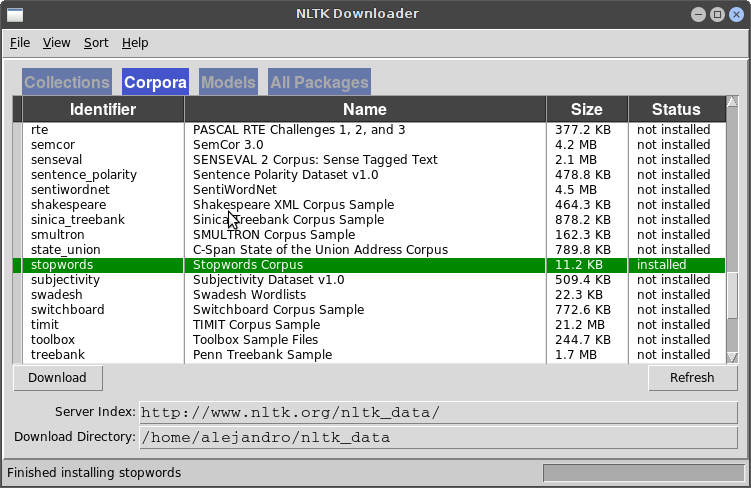
\includegraphics[width=0.8\textwidth]{stopwords_download}
\end{center}
\begin{itemize}
	\item Una vez que aparezca la pantalla de descargas vayan a la sección de \textbf{Corpora} y descarguen \textbf{stopwords}, que como verán, son listas de palabras funcionales en varios idiomas.
\end{itemize}
}



\frame{
\frametitle{NLTK}
\framesubtitle{Palabras funcionales}
\small
\begin{itemize}
	\item Y ahora que ya descargamos las listas, podemos cerrar esa ventana.
	\item A partir de ahora podemos usar las listas de \emph{stopwords} de NLTK. Veamos que palabras tiene para el español.
\end{itemize}
\colorbox{source}{\parbox{\textwidth}{
\ttfamily
\small
\mbox{}\\
\textbf{\textcolor{RoyalBlue}{import}}\ nltk \\
\mbox{} \\
\mbox{}palabras$\_$funcionales\textcolor{BrickRed}{=}nltk\textcolor{BrickRed}{.}corpus\textcolor{BrickRed}{.}stopwords\textcolor{BrickRed}{.}\textbf{\textcolor{Black}{words}}\textcolor{BrickRed}{(}\texttt{\textcolor{Red}{"{}spanish"{}}}\textcolor{BrickRed}{)} \\
\mbox{} \\
\mbox{}\textbf{\textcolor{Blue}{for}}\ palabras$\_$funcional\ \textbf{\textcolor{Blue}{in}}\ palabras$\_$funcionales\textcolor{BrickRed}{:} \\
\mbox{}\ \ \ \ \ \ \ \ \textbf{\textcolor{Blue}{print}}\textcolor{BrickRed}{(}palabras$\_$funcional\textcolor{BrickRed}{)} \\
\mbox{}
}}
}




\frame{
\frametitle{NLTK}
\framesubtitle{Palabras funcionales}
\colorbox{source}{\parbox{\textwidth}{
\ttfamily
\footnotesize
\mbox{}\\
\textbf{\textcolor{RoyalBlue}{import}}\ nltk \\
\mbox{} \\
\mbox{}carpeta$\_$nombre\textcolor{BrickRed}{=}\texttt{\textcolor{Red}{"{}C:\textbackslash{}\textbackslash{}Users\textbackslash{}\textbackslash{}user\textbackslash{}\textbackslash{}Desktop\textbackslash{}\textbackslash{}Documentos\textbackslash{}\textbackslash{}"{}}} \\
\mbox{}archivo$\_$nombre\textcolor{BrickRed}{=}\texttt{\textcolor{Red}{"{}P$\_$IFT$\_$290216$\_$73$\_$Acc.txt"{}}} \\
\mbox{} \\
\mbox{}with\ \textbf{\textcolor{Black}{open}}\textcolor{BrickRed}{(}carpeta$\_$nombre\textcolor{BrickRed}{+}archivo$\_$nombre\textcolor{BrickRed}{,}\texttt{\textcolor{Red}{"{}r"{}}}\textcolor{BrickRed}{)}\ as\ archivo\textcolor{BrickRed}{:} \\
\mbox{}\ \ \ \ \ \ \ \ texto\textcolor{BrickRed}{=}archivo\textcolor{BrickRed}{.}\textbf{\textcolor{Black}{read}}\textcolor{BrickRed}{()} \\
\mbox{}\ \ \ \ \ \ \ \  \\
\mbox{}palabras$\_$funcionales\textcolor{BrickRed}{=}nltk\textcolor{BrickRed}{.}corpus\textcolor{BrickRed}{.}stopwords\textcolor{BrickRed}{.}\textbf{\textcolor{Black}{words}}\textcolor{BrickRed}{(}\texttt{\textcolor{Red}{"{}spanish"{}}}\textcolor{BrickRed}{)} \\
\mbox{} \\
\mbox{}tokens\textcolor{BrickRed}{=}nltk\textcolor{BrickRed}{.}\textbf{\textcolor{Black}{word$\_$tokenize}}\textcolor{BrickRed}{(}texto\textcolor{BrickRed}{,}\texttt{\textcolor{Red}{"{}spanish"{}}}\textcolor{BrickRed}{)} \\
\mbox{} \\
\mbox{}tokens$\_$limpios\textcolor{BrickRed}{=[]} \\
\mbox{}\textbf{\textcolor{Blue}{for}}\ token\ \textbf{\textcolor{Blue}{in}}\ tokens\textcolor{BrickRed}{:} \\
\mbox{}\ \ \ \ \ \ \ \ \ \ \ \ \textbf{\textcolor{Blue}{if}}\ token\ \textbf{\textcolor{Blue}{not}}\ \textbf{\textcolor{Blue}{in}}\ palabras$\_$funcionales\textcolor{BrickRed}{:} \\
\mbox{}\ \ \ \ \ \ \ \ \ \ \ \ \ \ \ \ \ \ \ \ tokens$\_$limpios\textcolor{BrickRed}{.}\textbf{\textcolor{Black}{append}}\textcolor{BrickRed}{(}token\textcolor{BrickRed}{)} \\
\mbox{} \\
\mbox{}\textbf{\textcolor{Blue}{print}}\textcolor{BrickRed}{(}\textbf{\textcolor{Black}{len}}\textcolor{BrickRed}{(}tokens\textcolor{BrickRed}{))} \\
\mbox{}\textbf{\textcolor{Blue}{print}}\textcolor{BrickRed}{(}\textbf{\textcolor{Black}{len}}\textcolor{BrickRed}{(}tokens$\_$limpios\textcolor{BrickRed}{))} \\
\mbox{}
}}
}
\note{
\begin{itemize}
	\item ¿Qué estamos haciendo aquí?
	\item Estamos filtrando las palabras funcionales y las quitamos del texto.
	\item Tenemos nuestra lista de tokens, dentro de la variable {\tt\textbf{tokens}}.
	\item Inmediatamente después, creamos una nueva variable: {\tt\textbf{tokens\_limpios}}. Que como pueden ver, es una lista vacía! El plan, es llenarla a continuación.
	\item Y para eso justamente está ese {\tt\textbf{for}}. Usamos un bucle que recorre todos los tokens de nuestro texto y verificamos si son palabras funcionales o no.
	\item Para ver si son palabras funcionales, usamos la instrucción {\tt\textbf{not in}} que como es de esperar, hace lo contrario a la instrucción {\tt\textbf{in}} (la recuerdan?).
\end{itemize}
}
\note{
\begin{itemize}
	\item En resumen, ese {\tt\textbf{if}}, ve si el token que se está revisando está dentro de la lista de palabras funcionales. Si NO lo está (por eso el {\tt\textbf{not in}}) entonces podemos decir que ese token no es una palabra funcional. Por lo tanto queremos que esté dentro de nuestra lista limpia de palabras funcionales.
	\item Una vez que la condición se cumple y que vemos que el token NO es una palabra funcional, lo agregamos a la lista que habíamos creado (a la lista de {\tt\textbf{tokens\_limpios}}) con la función {\tt\textbf{append()}}. Esa función lo que hace es agregar el valor que le damos al final de la lista.
	\item Por último, mostramos en pantalla las longitudes de ambas listas de tokens, para que vean la diferencia de tamaño entre la que tiene palabras funcionales y la que no.
\end{itemize}
}



\frame{
\frametitle{NLTK}
\framesubtitle{Palabras funcionales}
\small
\begin{itemize}
	\item Podemos también obtener las gráficas de los nuevos datos sin palabras funcionales.
	\item Por cierto, quizá notaron en el ejemplo anterior que mostramos en pantalla (con {\tt\textbf{print()}}) el resultado directo de una función, sin asignarlo antes a una variable. En Python podemos hacer poner una cadena de funciones y usar los resultados inmediatamente, incluso podemos hacer algo tan drástico como el siguiente ejemplo, pero por norma general, no se recomienda, se vuelve poco legible y no se pueden recuperar los datos intermedios.
\end{itemize}
\colorbox{source}{\parbox{\textwidth}{
\ttfamily
\mbox{}\\
\textit{\textcolor{Brown}{\#\ Después\ del\ ejemplo\ anterior...}} \\
\mbox{} \\
\mbox{}nltk\textcolor{BrickRed}{.}\textbf{\textcolor{Black}{FreqDist}}\textcolor{BrickRed}{(}nltk\textcolor{BrickRed}{.}\textbf{\textcolor{Black}{Text}}\textcolor{BrickRed}{(}tokens$\_$limpios\textcolor{BrickRed}{)).}\textbf{\textcolor{Black}{plot}}\textcolor{BrickRed}{(}\textcolor{Purple}{40}\textcolor{BrickRed}{)} \\
\mbox{}
}}
}



\frame{
\frametitle{NLTK}
\framesubtitle{Palabras funcionales}
\small
\begin{itemize}
	\item Como pueden observar, aún hay elementos muy frecuentes que sería útil quitar, como los sinos de puntuación.
	\item Usaré este punto para explicarles un detalle sobre el texto que no había mencionado antes. Y es que se puede comportar un poco como una lista de letras.
	\item El ejemplo siguiente es una solución ingenua para quitar los signos de puntuación, es decir, es muy simple, pero no es la solución ideal ya que esto quitará más cosas solamente los signos de puntuación, pero depende del objetivo final, puede que la pérdida no sea importante.
\end{itemize}
}





\frame{
\frametitle{NLTK}
\framesubtitle{Palabras funcionales}
\colorbox{source}{\parbox{\textwidth}{
\ttfamily
\footnotesize
\mbox{}\\
\textbf{\textcolor{RoyalBlue}{import}}\ nltk \\
\mbox{} \\
\mbox{}carpeta$\_$nombre\textcolor{BrickRed}{=}\texttt{\textcolor{Red}{"{}C:\textbackslash{}\textbackslash{}Users\textbackslash{}\textbackslash{}user\textbackslash{}\textbackslash{}Desktop\textbackslash{}\textbackslash{}Documentos\textbackslash{}\textbackslash{}"{}}} \\
\mbox{}archivo$\_$nombre\textcolor{BrickRed}{=}\texttt{\textcolor{Red}{"{}P$\_$IFT$\_$290216$\_$73$\_$Acc.txt"{}}} \\
\mbox{} \\
\mbox{}with\ \textbf{\textcolor{Black}{open}}\textcolor{BrickRed}{(}carpeta$\_$nombre\textcolor{BrickRed}{+}archivo$\_$nombre\textcolor{BrickRed}{,}\texttt{\textcolor{Red}{"{}r"{}}}\textcolor{BrickRed}{)}\ as\ archivo\textcolor{BrickRed}{:} \\
\mbox{}\ \ \ \ \ \ \ \ texto\textcolor{BrickRed}{=}archivo\textcolor{BrickRed}{.}\textbf{\textcolor{Black}{read}}\textcolor{BrickRed}{()} \\
\mbox{}\ \ \ \ \ \ \ \  \\
\mbox{}palabras$\_$funcionales\textcolor{BrickRed}{=}nltk\textcolor{BrickRed}{.}corpus\textcolor{BrickRed}{.}stopwords\textcolor{BrickRed}{.}\textbf{\textcolor{Black}{words}}\textcolor{BrickRed}{(}\texttt{\textcolor{Red}{"{}spanish"{}}}\textcolor{BrickRed}{)} \\
\mbox{} \\
\mbox{}tokens\textcolor{BrickRed}{=}nltk\textcolor{BrickRed}{.}\textbf{\textcolor{Black}{word$\_$tokenize}}\textcolor{BrickRed}{(}texto\textcolor{BrickRed}{,}\texttt{\textcolor{Red}{"{}spanish"{}}}\textcolor{BrickRed}{)} \\
\mbox{} \\
\mbox{}tokens$\_$limpios\textcolor{BrickRed}{=[]} \\
\mbox{}\textbf{\textcolor{Blue}{for}}\ token\ \textbf{\textcolor{Blue}{in}}\ tokens\textcolor{BrickRed}{:} \\
\mbox{}\ \ \ \ \ \ \ \ \textbf{\textcolor{Blue}{if}}\ token\ \textbf{\textcolor{Blue}{not}}\ \textbf{\textcolor{Blue}{in}}\ palabras$\_$funcionales\textcolor{BrickRed}{:} \\
\mbox{}\ \ \ \ \ \ \ \ \ \ \ \ \ \ \ \ \textbf{\textcolor{Blue}{if}}\ \textbf{\textcolor{Black}{len}}\textcolor{BrickRed}{(}token\textcolor{BrickRed}{)}\ \textcolor{BrickRed}{\textgreater{}}\ \textcolor{Purple}{1}\textcolor{BrickRed}{:} \\
\mbox{}\ \ \ \ \ \ \ \ \ \ \ \ \ \ \ \ \ \ \ \ \ \ \ \ tokens$\_$limpios\textcolor{BrickRed}{.}\textbf{\textcolor{Black}{append}}\textcolor{BrickRed}{(}token\textcolor{BrickRed}{)} \\
\mbox{} \\
\mbox{}nltk\textcolor{BrickRed}{.}\textbf{\textcolor{Black}{FreqDist}}\textcolor{BrickRed}{(}nltk\textcolor{BrickRed}{.}\textbf{\textcolor{Black}{Text}}\textcolor{BrickRed}{(}tokens$\_$limpios\textcolor{BrickRed}{)).}\textbf{\textcolor{Black}{plot}}\textcolor{BrickRed}{(}\textcolor{Purple}{40}\textcolor{BrickRed}{)} \\
\mbox{}
}}
}
\note{
\vspace{-0.3cm}
\begin{itemize}
	\item El cambio está en el bucle en el que se llena la lista {\tt\textbf{tokens\_limpios}}. Agregamos un {\tt\textbf{if}} dentro del que ya había.
	\item Esto quiere decir que no bastará ahora con que el token no sea una palabra funcional, si no que ahora, se busca también que: {\tt\textbf{len(token) > 1}}. Y esto quiere decir que el token tenga MAS de una letra.
	\item La función {\tt\textbf{len()}} la habíamos usado para ver el tamaño de una lista, pero también la podemos usar para ver cuántas letras tiene una palabra, el texto en Python se comporta como una lista de letras.
	\item En este nuevo programa, si se cumple que el token NO es una palabra funcional Y que tiene MÁS de 1 letra, entonces se agrega a la lista de tokens limpios.
	\item Esto va a eliminar los símbolos, aunque también elimina otras cosas, hay que tener eso en cuenta.
\end{itemize}
}




\frame{
\frametitle{NLTK}
\framesubtitle{Palabras funcionales}
\small
\begin{itemize}
	\item Del ejemplo anterior, podemos ver como las palabras "{}limpias"{} más comunes, ya nos dan información importante sobre un texto.
	\item Por cierto, para ustedes que no tienen que ahorrar espacio, recuerden que esto no es recomendable:
\end{itemize}
\colorbox{source}{\parbox{\textwidth}{
\ttfamily
\mbox{}\\
\mbox{}nltk\textcolor{BrickRed}{.}\textbf{\textcolor{Black}{FreqDist}}\textcolor{BrickRed}{(}nltk\textcolor{BrickRed}{.}\textbf{\textcolor{Black}{Text}}\textcolor{BrickRed}{(}tokens$\_$limpios\textcolor{BrickRed}{)).}\textbf{\textcolor{Black}{plot}}\textcolor{BrickRed}{(}\textcolor{Purple}{40}\textcolor{BrickRed}{)} \\
\mbox{}
}}
\begin{itemize}
	\item Es mejor esto:
\end{itemize}
\colorbox{source}{\parbox{\textwidth}{
\ttfamily
\mbox{}\\
\mbox{}texto$\_$limpio$\_$nltk\textcolor{BrickRed}{=}nltk\textcolor{BrickRed}{.}\textbf{\textcolor{Black}{Text}}\textcolor{BrickRed}{(}tokens$\_$limpios\textcolor{BrickRed}{)} \\
\mbox{}distribucion$\_$limpia\textcolor{BrickRed}{=}nltk\textcolor{BrickRed}{.}\textbf{\textcolor{Black}{FreqDist}}\textcolor{BrickRed}{(}texto$\_$limpio$\_$nltk\textcolor{BrickRed}{)} \\
\mbox{} \\
\mbox{}distribucion$\_$limpia\textcolor{BrickRed}{.}\textbf{\textcolor{Black}{plot}}\textcolor{BrickRed}{(}\textcolor{Purple}{40}\textcolor{BrickRed}{)} \\
\mbox{}
}}
}




\frame{
\frametitle{NLTK}
\framesubtitle{Colocaciones}
\vspace{-0.35cm}
\small
\begin{itemize}
	\item Las colocaciones son secuencias de palabras que ocurren juntas de una forma inusualmente frecuente.
	\item NLTK tiene una función particular para obtener las colocaciones de un texto.
\end{itemize}
\colorbox{source}{\parbox{\textwidth}{
\ttfamily
\mbox{}\\
\textit{\textcolor{Brown}{\#\ Aquí\ ya\ tenemos\ tokens\ y\ tokens$\_$limpios}} \\
\mbox{} \\
\mbox{}texto$\_$nltk\textcolor{BrickRed}{=}nltk\textcolor{BrickRed}{.}\textbf{\textcolor{Black}{Text}}\textcolor{BrickRed}{(}tokens\textcolor{BrickRed}{)} \\
\mbox{}texto$\_$limpio$\_$nltk\textcolor{BrickRed}{=}nltk\textcolor{BrickRed}{.}\textbf{\textcolor{Black}{Text}}\textcolor{BrickRed}{(}tokens$\_$limpios\textcolor{BrickRed}{)} \\
\mbox{} \\
\mbox{}texto$\_$nltk\textcolor{BrickRed}{.}\textbf{\textcolor{Black}{collocations}}\textcolor{BrickRed}{()} \\
\mbox{}\textbf{\textcolor{Blue}{print}}\textcolor{BrickRed}{()} \\
\mbox{}texto$\_$limpio$\_$nltk\textcolor{BrickRed}{.}\textbf{\textcolor{Black}{collocations}}\textcolor{BrickRed}{()} \\
\mbox{}
}}
\begin{itemize}
	\item Se puede usar tanto el texto completo como el "{}limpio"{}, ambos dan información que puede ser útil, como "{}rubro citado"{} o "{}S.A. C.V."{} "{}Ciudad México"{}. Que aparecen solo en uno de los dos.
\end{itemize}
}
\note{
\begin{itemize}
	\item La función {\tt\textbf{collocations()}} de NLTK también es una de esas funciones que escribe por si misma en la pantalla, no es necesario asignarla a una variable.
\end{itemize}
}



\frame{
\frametitle{NLTK}
\framesubtitle{Etiquetado PoS}
\vspace{-0.35cm}
\small
\begin{itemize}
	\item Un recurso muy útil para el PLN es el etiquetado PoS (de \emph{Part of Speech}).
	\item Con esta herramienta, la computadora hace su mejor esfuerzo por asignarle a cada palabra de un texto la parte de la oración que le corresponde (sustantivo, verbo, adjetivo, determinante, etc.)
	\item NLTK cuenta con un etiquetador PoS. Desafortunadamente, es solo para inglés.
	\item Afortunadamente, también tiene acceso a un etiquetador externo (de Stanford) que si es capaz de manejar el español.
	\item Esta herramienta no la tiene por defecto, y al ser externa tampoco se descarga desde el sistema de descarga que hemos estado usando hasta ahora.
	\item \url{https://nlp.stanford.edu/software/tagger.shtml}
\end{itemize}
}




\frame{
\frametitle{NLTK}
\framesubtitle{Etiquetado PoS}
\begin{itemize}
	\item En la página de Stanford podemos encontrar toda la información sobre el etiquetador y ligas de descarga.
\end{itemize}
\centering
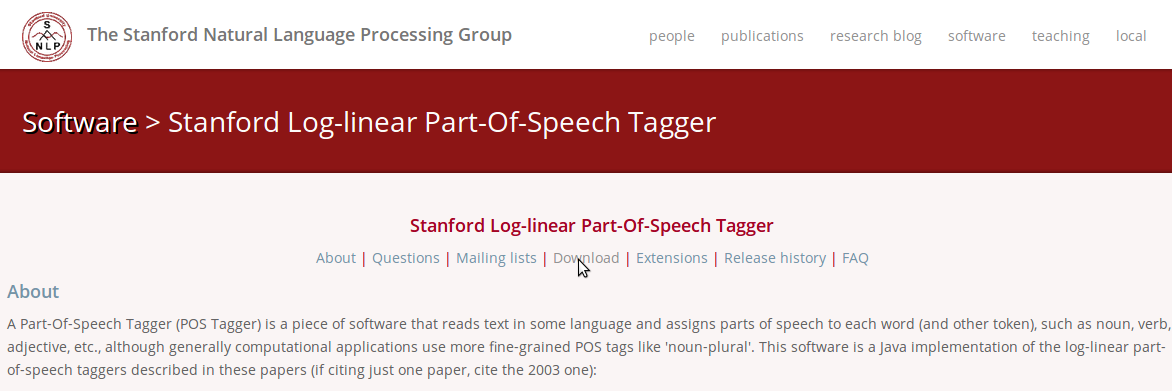
\includegraphics[width=\textwidth]{stanford_home}
}




\frame{
\frametitle{NLTK}
\framesubtitle{Etiquetado PoS}
\small
\begin{itemize}
	\item La descarga básica de su etiquetador también funciona solo con inglés, así que necesitamos la descarga completa, es la segunda liga.
	\item Esto va a descargar un archivo comprimido, es importante que lo descompriman y que recuerden donde lo colocan. Recuerden la forma de obtener rutas completas, será necesario para usarlo.
\end{itemize}
\centering
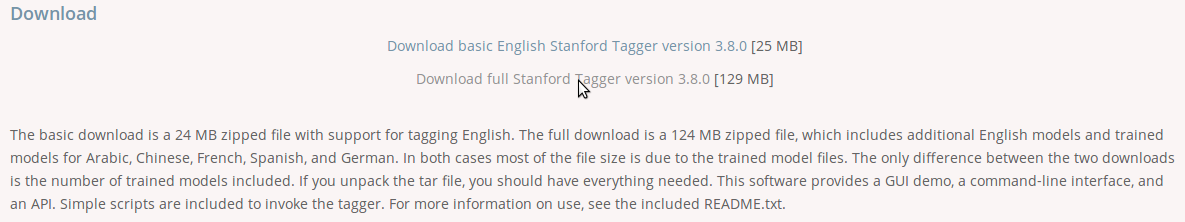
\includegraphics[width=\textwidth]{stanford_download}
}




\frame{
\frametitle{NLTK}
\framesubtitle{Etiquetado PoS}
\begin{itemize}
	\item Una vez que hayan descargado y descomprimido el zip, hay dos archivos que deben localizar.
	\item El primero está directamente dentro de la carpeta que acaban de descomprimir, se llama {\tt\textbf{stanford-postagger.jar}}.
	\item El segundo, está dentro de la carpeta {\tt\textbf{models}}, y su nombre es {\tt\textbf{spanish.tagger}}  sin nada más.
	\item Para ambos archivos van a necesitar la ruta completa para usarlos con Python y NLTK.
\end{itemize}
}




\frame{
\frametitle{NLTK}
\framesubtitle{Etiquetado PoS}
\small
\begin{itemize}
	\item La función {\tt\textbf{StanfordPOSTagger()}} recibe de parámetros los archivos que obtuvimos, primero el {\tt\textbf{spanish.tagger}}, luego el {\tt\textbf{stanford-postagger.jar}}.
\end{itemize}
\colorbox{source}{\parbox{\textwidth}{
\ttfamily
\footnotesize
\mbox{}\\
\textbf{\textcolor{RoyalBlue}{from}}\ nltk\textcolor{BrickRed}{.}tag\ \textbf{\textcolor{RoyalBlue}{import}}\ StanfordPOSTagger \\
\mbox{} \\
\mbox{}\textit{\textcolor{Brown}{\#\ Aquí\ obtenemos\ la\ lista\ de\ tokens\ en\ "{}tokens"{}}} \\
\mbox{} \\
\mbox{}tagger\textcolor{BrickRed}{=}\texttt{\textcolor{Red}{"{}C:\textbackslash{}\textbackslash{}Users\textbackslash{}\textbackslash{}user\textbackslash{}\textbackslash{}Downloads\textbackslash{}\textbackslash{}...\textbackslash{}\textbackslash{}spanish.tagger"{}}} \\
\mbox{}jar\textcolor{BrickRed}{=}\texttt{\textcolor{Red}{"{}C:\textbackslash{}\textbackslash{}Users\textbackslash{}\textbackslash{}user\textbackslash{}\textbackslash{}Downloads\textbackslash{}\textbackslash{}...\textbackslash{}\textbackslash{}stanford-postagger.jar"{}}} \\
\mbox{} \\
\mbox{}etiquetador\textcolor{BrickRed}{=}\textbf{\textcolor{Black}{StanfordPOSTagger}}\textcolor{BrickRed}{(}tagger\textcolor{BrickRed}{,}jar\textcolor{BrickRed}{)} \\
\mbox{}etiquetas\textcolor{BrickRed}{=}etiquetador\textcolor{BrickRed}{.}\textbf{\textcolor{Black}{tag}}\textcolor{BrickRed}{(}tokens\textcolor{BrickRed}{)} \\
\mbox{} \\
\mbox{}\textbf{\textcolor{Blue}{for}}\ etiqueta\ \textbf{\textcolor{Blue}{in}}\ etiquetas\textcolor{BrickRed}{:} \\
\mbox{}\ \ \ \ \ \ \ \ \textbf{\textcolor{Blue}{print}}\textcolor{BrickRed}{(}etiqueta\textcolor{BrickRed}{)} \\
\mbox{}
}}
}
\note{
\begin{itemize}
	\item Lo mejor es importar el etiquetador externo de nltk como se muestra para no tener que usar toda la ruta.
\end{itemize}
}




\frame{
\frametitle{NLTK}
\framesubtitle{Etiquetado PoS}
\small
\begin{itemize}
	\item Con esa información, el {\tt\textbf{StanfordPOSTagger()}} crea un etiquetador que luego podemos utilizar para etiquetar nuestra lista de tokens. En este caso, es mejor utilizar la lista que no está "{}limpia"{}.
\end{itemize}
\colorbox{source}{\parbox{\textwidth}{
\ttfamily
\footnotesize
\mbox{}\\
\textbf{\textcolor{RoyalBlue}{from}}\ nltk\textcolor{BrickRed}{.}tag\ \textbf{\textcolor{RoyalBlue}{import}}\ StanfordPOSTagger \\
\mbox{} \\
\mbox{}\textit{\textcolor{Brown}{\#\ Aquí\ obtenemos\ la\ lista\ de\ tokens\ en\ "{}tokens"{}}} \\
\mbox{} \\
\mbox{}tagger\textcolor{BrickRed}{=}\texttt{\textcolor{Red}{"{}C:\textbackslash{}\textbackslash{}Users\textbackslash{}\textbackslash{}user\textbackslash{}\textbackslash{}Downloads\textbackslash{}\textbackslash{}...\textbackslash{}\textbackslash{}spanish.tagger"{}}} \\
\mbox{}jar\textcolor{BrickRed}{=}\texttt{\textcolor{Red}{"{}C:\textbackslash{}\textbackslash{}Users\textbackslash{}\textbackslash{}user\textbackslash{}\textbackslash{}Downloads\textbackslash{}\textbackslash{}...\textbackslash{}\textbackslash{}stanford-postagger.jar"{}}} \\
\mbox{} \\
\mbox{}etiquetador\textcolor{BrickRed}{=}\textbf{\textcolor{Black}{StanfordPOSTagger}}\textcolor{BrickRed}{(}tagger\textcolor{BrickRed}{,}jar\textcolor{BrickRed}{)} \\
\mbox{}etiquetas\textcolor{BrickRed}{=}etiquetador\textcolor{BrickRed}{.}\textbf{\textcolor{Black}{tag}}\textcolor{BrickRed}{(}tokens\textcolor{BrickRed}{)} \\
\mbox{} \\
\mbox{}\textbf{\textcolor{Blue}{for}}\ etiqueta\ \textbf{\textcolor{Blue}{in}}\ etiquetas\textcolor{BrickRed}{:} \\
\mbox{}\ \ \ \ \ \ \ \ \textbf{\textcolor{Blue}{print}}\textcolor{BrickRed}{(}etiqueta\textcolor{BrickRed}{)} \\
\mbox{}
}}
}
\note{
\begin{itemize}
	\item Las etiquetas se regresan en una lista, cada elemento tiene el token junto con su etiqueta.
	\item Notarán que cada pareja (token-etiqueta) dentro de la lista se encuentra entre paréntesis, esto en realidad quiere decir que también están formando una lista.
	\item Ok, no una lista, sino una tupla, la única diferencia entre ambas es que estas tuplas NO las pueden modificar, digamos que son de solo lectura. Pero a fin de cuentas, pueden ingresar a sus datos por índices igual que lo harían con una lista.
	\item Así que, si usan por ejemplo {\tt\textbf{etiqueta[0]}} obtendrán el token únicamente, si usan {\tt\textbf{etiqueta[1]}} obtendrán solo la etiqueta.
\end{itemize}
}




\frame{
\frametitle{NLTK}
\framesubtitle{Etiquetado PoS}
\vspace{-0.35cm}
\small
\begin{itemize}
	\item ¿Y esas etiquetas qué?
	\item Cada etiqueta tiene un significado, en la página \url{https://nlp.stanford.edu/software/spanish-faq.shtml\#tagset} pueden encontrar las etiquetas con sus significados y ejemplos.
\end{itemize}
\centering
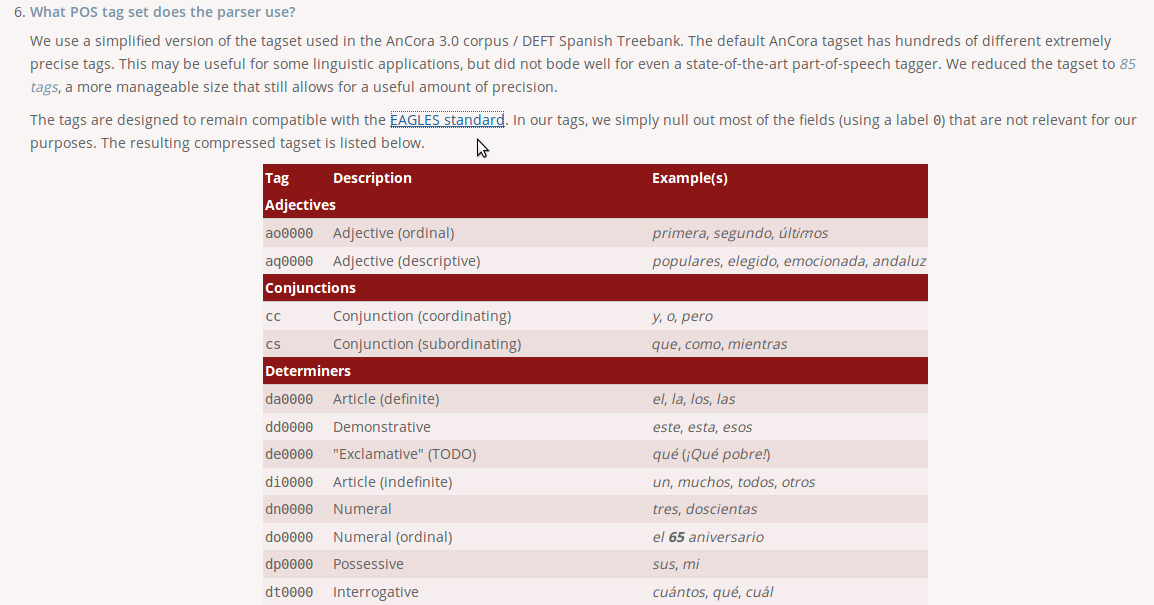
\includegraphics[width=\textwidth]{stanford_tags}
}



\end{document}
